% Options for packages loaded elsewhere
\PassOptionsToPackage{unicode}{hyperref}
\PassOptionsToPackage{hyphens}{url}
%
\documentclass[
]{article}
\usepackage{amsmath,amssymb}
\usepackage{iftex}
\ifPDFTeX
  \usepackage[T1]{fontenc}
  \usepackage[utf8]{inputenc}
  \usepackage{textcomp} % provide euro and other symbols
\else % if luatex or xetex
  \usepackage{unicode-math} % this also loads fontspec
  \defaultfontfeatures{Scale=MatchLowercase}
  \defaultfontfeatures[\rmfamily]{Ligatures=TeX,Scale=1}
\fi
\usepackage{lmodern}
\ifPDFTeX\else
  % xetex/luatex font selection
\fi
% Use upquote if available, for straight quotes in verbatim environments
\IfFileExists{upquote.sty}{\usepackage{upquote}}{}
\IfFileExists{microtype.sty}{% use microtype if available
  \usepackage[]{microtype}
  \UseMicrotypeSet[protrusion]{basicmath} % disable protrusion for tt fonts
}{}
\makeatletter
\@ifundefined{KOMAClassName}{% if non-KOMA class
  \IfFileExists{parskip.sty}{%
    \usepackage{parskip}
  }{% else
    \setlength{\parindent}{0pt}
    \setlength{\parskip}{6pt plus 2pt minus 1pt}}
}{% if KOMA class
  \KOMAoptions{parskip=half}}
\makeatother
\usepackage{xcolor}
\usepackage[margin=1in]{geometry}
\usepackage{longtable,booktabs,array}
\usepackage{calc} % for calculating minipage widths
% Correct order of tables after \paragraph or \subparagraph
\usepackage{etoolbox}
\makeatletter
\patchcmd\longtable{\par}{\if@noskipsec\mbox{}\fi\par}{}{}
\makeatother
% Allow footnotes in longtable head/foot
\IfFileExists{footnotehyper.sty}{\usepackage{footnotehyper}}{\usepackage{footnote}}
\makesavenoteenv{longtable}
\usepackage{graphicx}
\makeatletter
\def\maxwidth{\ifdim\Gin@nat@width>\linewidth\linewidth\else\Gin@nat@width\fi}
\def\maxheight{\ifdim\Gin@nat@height>\textheight\textheight\else\Gin@nat@height\fi}
\makeatother
% Scale images if necessary, so that they will not overflow the page
% margins by default, and it is still possible to overwrite the defaults
% using explicit options in \includegraphics[width, height, ...]{}
\setkeys{Gin}{width=\maxwidth,height=\maxheight,keepaspectratio}
% Set default figure placement to htbp
\makeatletter
\def\fps@figure{htbp}
\makeatother
\setlength{\emergencystretch}{3em} % prevent overfull lines
\providecommand{\tightlist}{%
  \setlength{\itemsep}{0pt}\setlength{\parskip}{0pt}}
\setcounter{secnumdepth}{5}
\newlength{\cslhangindent}
\setlength{\cslhangindent}{1.5em}
\newlength{\csllabelwidth}
\setlength{\csllabelwidth}{3em}
\newlength{\cslentryspacingunit} % times entry-spacing
\setlength{\cslentryspacingunit}{\parskip}
\newenvironment{CSLReferences}[2] % #1 hanging-ident, #2 entry spacing
 {% don't indent paragraphs
  \setlength{\parindent}{0pt}
  % turn on hanging indent if param 1 is 1
  \ifodd #1
  \let\oldpar\par
  \def\par{\hangindent=\cslhangindent\oldpar}
  \fi
  % set entry spacing
  \setlength{\parskip}{#2\cslentryspacingunit}
 }%
 {}
\usepackage{calc}
\newcommand{\CSLBlock}[1]{#1\hfill\break}
\newcommand{\CSLLeftMargin}[1]{\parbox[t]{\csllabelwidth}{#1}}
\newcommand{\CSLRightInline}[1]{\parbox[t]{\linewidth - \csllabelwidth}{#1}\break}
\newcommand{\CSLIndent}[1]{\hspace{\cslhangindent}#1}
\usepackage{booktabs}
\usepackage{longtable}
\usepackage{array}
\usepackage{multirow}
\usepackage{wrapfig}
\usepackage{float}
\usepackage{colortbl}
\usepackage{pdflscape}
\usepackage{tabu}
\usepackage{threeparttable}
\usepackage{threeparttablex}
\usepackage[normalem]{ulem}
\usepackage{makecell}
\usepackage{xcolor}
\ifLuaTeX
  \usepackage{selnolig}  % disable illegal ligatures
\fi
\IfFileExists{bookmark.sty}{\usepackage{bookmark}}{\usepackage{hyperref}}
\IfFileExists{xurl.sty}{\usepackage{xurl}}{} % add URL line breaks if available
\urlstyle{same}
\hypersetup{
  pdftitle={NHANES Blood Pressure-Based Mortality Risk - Appendix},
  pdfauthor={Rscripts by Hamish Patten, DW Bester and David Steinsaltz},
  hidelinks,
  pdfcreator={LaTeX via pandoc}}

\title{NHANES Blood Pressure-Based Mortality Risk - Appendix}
\author{Rscripts by Hamish Patten, DW Bester and David Steinsaltz}
\date{10/10/2023}

\begin{document}
\maketitle

{
\setcounter{tocdepth}{3}
\tableofcontents
}
\hypertarget{appendix-a-the-data}{%
\section{Appendix A -- The data}\label{appendix-a-the-data}}

\begin{figure}

{\centering 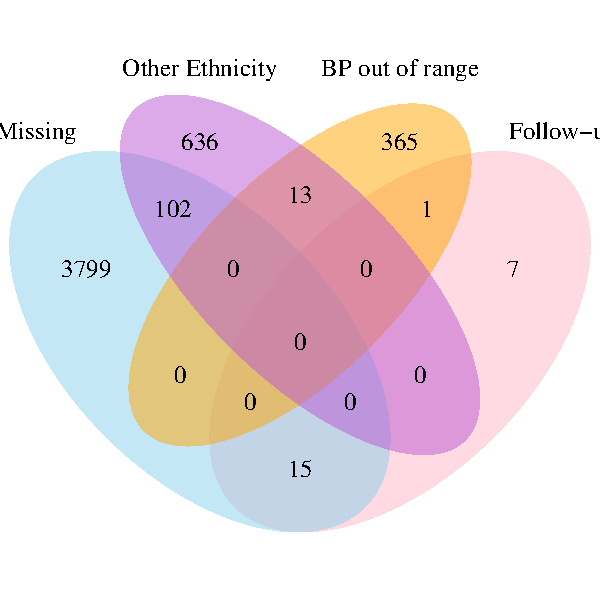
\includegraphics{NHANES-BP-Appendix_files/figure-latex/Venn1-1} 

}

\caption{Venn diagram of subjects excluded from the analysis.}\label{fig:Venn1}
\end{figure}

\hypertarget{exclusions}{%
\subsection{Exclusions}\label{exclusions}}

There were 19592 subjects in the initial data set.
Of these 4573 were excluded because they had missing data or were not followed up, or belonged to the ``Other'' ethnic group.
This left 15019 subjects for further consideration.
A small number of subjects were excluded because their blood pressure measurements were outside the normal range, as described below in section \ref{sec:BPrange}.
In the end there were 14654 subjects in the analysis data set.
A Venn diagram of the different causes of exclusion is given in figure \ref{fig:Venn1}.
We will refer to this as the ``full population''.
Of these, 9008 had a computable FRS score.
We call this the ``FRS population''.

\hypertarget{addressing-errors-in-blood-pressure-measurement}{%
\subsection{Addressing errors in blood pressure measurement}\label{addressing-errors-in-blood-pressure-measurement}}

The blood pressure measurement or recording errors were found particularly in the home measurements.
While these did not destroy the usefulness of the home measurements, they did require some attention and decisions for how to work with these defects.
We also consider them inherently interesting, and worth registering for future researchers working on these or similar data.
In particular, the problem we have called ``dependent replication'' was entirely unexpected, although not unprecedented, and is of particular concern to researchers trying to estimate individual variation in clinically relevant measures.

\hypertarget{sec:lastdigit}{%
\subsubsection{Last-digit preference}\label{sec:lastdigit}}

Mild tendency for observers to prefer certain last digits in reporting BP measurements has been reported in other studies, though an analysis of the 1999 wave of NHANES reported no last-digit preference (Ostchega et al. 2003).\\
The last-digit preference in NHANES III, on the other hand, is substantial, with about 26.7\% of all the clinic-measured systolic BP measurements ending in 0, but only about 31.9\% ending in 4 or 6. Because the shifts due to last-digit preference are presumably small, we expect them to have little effect on the main effects that we are examining in this paper, but they do increase the probability of two measurements being rounded to the same value, something that needs to be taken into account in examining the problem of dependent replication.

\begin{table}[!h]

\caption{\label{tab:digit-summary}Summary data for BP end digits}
\centering
\begin{tabular}[t]{llrrrrr}
\toprule
Place & Sys/Dias & 0 & 2 & 4 & 6 & 8\\
\midrule
Home & Systolic & 0.240 & 0.199 & 0.159 & 0.169 & 0.233\\
Home & Diastolic & 0.186 & 0.179 & 0.198 & 0.217 & 0.219\\
Clinic & Systolic & 0.267 & 0.188 & 0.160 & 0.159 & 0.226\\
Clinic & Diastolic & 0.192 & 0.189 & 0.209 & 0.212 & 0.198\\
\bottomrule
\end{tabular}
\end{table}

\hypertarget{sec:pseudorep}{%
\subsubsection{Dependent replicates}\label{sec:pseudorep}}

While the protocol calls for each subject to have three independent BP measures taken, it is not impossible that the observers may have been influenced by one measure in recording the next.
This could happen in either direction: later measurements could be pulled closer to the first, or there could be an inclination to avoid repeated measures.
This is relevant, because erroneously repeated measures would artificially decrease the variance of the three measurements, and avoiding repeated measures would have the opposite effect.

The end-digit bias may be expected to have an effect here, since it influences the probability of two measurements being rounded to the same value.
We begin by noting the standard deviations for measurements of individual subjects as given in the column `Mean of SD' in Table \ref{tab:sd-summary}.
The column `Prob all rep' gives the theoretical probability that two of the three measurements for a subject would have the same value, if the measurements were independent and normally distributed with the given standard deviation (adjusted for the rounding), and assuming that rounding to particular digits is done in proportion to the fractions listed in Table \ref{tab:digit-summary}.
The column `Prob 2 rep' gives the probability that two of the three measurements would have the same value, under the same conditions.
The column `Frac all rep' gives the observed fraction of subjects for whom all three measurements were equal, and `Frac 2 rep' gives the fraction for whom two of the three measurements were equal.
The observed fractions for three equal measurements are all very close to the theoretical probabilities, but the observed fractions for two equal measurements are substantially lower than the theoretical probabilities.
(For comparison, a 95\% probability range for the fraction of subjects with two equal measurements is about \(\pm 0.008\).)

In Figure \ref{fig:examinerPlot}, we show the fraction of subjects with two equal measurements, by examiner, blocked by place and type.
We see that the fraction of subjects with two equal measurements varies substantially by examiner, and that the variation is greater for the systolic than for the diastolic measurements.

\begin{table}[!h]

\caption{\label{tab:sd-summary}Summary data for repeated measures}
\centering
\begin{tabular}[t]{llrrrrr}
\toprule
Place & Sys/Dias & Mean of SD & Frac all rep & Prob all rep & Frac 2 rep & Prob 2 rep\\
\midrule
Home & Systolic & 2.739 & 0.050 & 0.048 & 0.432 & 0.510\\
Home & Diastolic & 2.343 & 0.063 & 0.061 & 0.488 & 0.564\\
Clinic & Systolic & 3.775 & 0.024 & 0.028 & 0.355 & 0.400\\
Clinic & Diastolic & 3.082 & 0.028 & 0.036 & 0.414 & 0.459\\
\bottomrule
\end{tabular}
\end{table}

We show the fraction of subjects with two equal measurements in figure 2, split by examiner, blocked by place and type.
We see that the fraction of subjects with two equal measurements varies substantially by examiner, and that the variation is greater for the systolic than for the diastolic measurements.

\begin{figure}
\centering
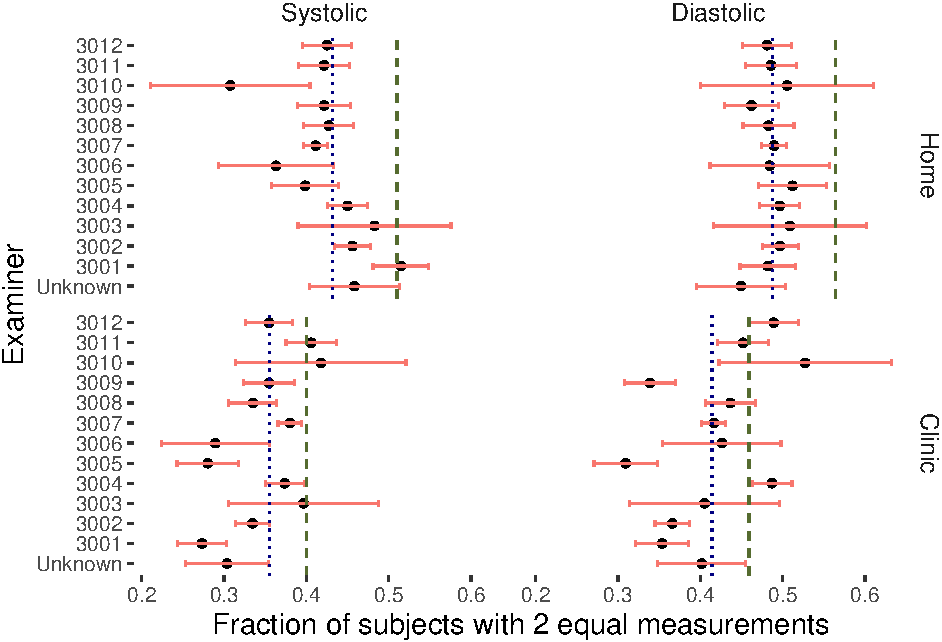
\includegraphics{NHANES-BP-Appendix_files/figure-latex/examinerPlot-1.pdf}
\caption{\label{fig:examinerPlot}Number of subjects with 2 equal measurements by examiner, blocked by place and type. Red band shows 95\% probability range. Vertical green dashed line shows expected fraction; blue dotted line shows observed fraction over all examiners.}
\end{figure}

\begin{figure}
\centering
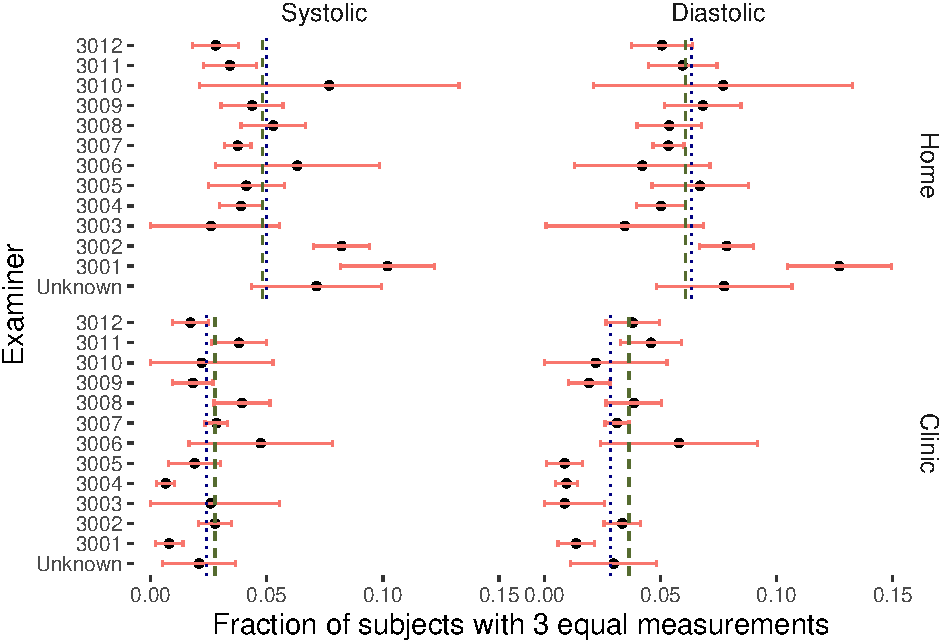
\includegraphics{NHANES-BP-Appendix_files/figure-latex/examinerPlot3-1.pdf}
\caption{\label{fig:examinerPlot3}Number of subjects with 3 equal measurements by examiner, blocked by place and type. Red band shows 95\% probability range. Vertical green dashed line shows expected fraction; blue dotted line shows observed fraction over all examiners.}
\end{figure}

In Figure \ref{fig:examinerPlot3}, we show the fraction of subjects with three equal measurements, by examiner, blocked by place and type.
Relative to the expected random fluctuations, we see that there is even more variation among the examiners.
One examiner (3001) produced consistently excessive numbers of triple repeats in Home measurements, and a deficit of triple repeats in Clinic measurements.

One further point to explore is the position of the two equal measures in a group of three.
If there are three independent measures, with two equal, each of the three has equal probability of being the odd one out.
On the other hand, if there is a trend in the measurements, then the second is least likely to be the odd one out.

In fact, what we observe is that it is the third measurement that is least likely to differ from the other two, while the first is most likely.
This is what we would expect if examiners sometimes either intentionally copied the second measurement into the space for the third, or unintentionally allowed themselves to be influenced into observing the same number.
The proportions are listed in Table \ref{tab:proportionChisq}, together with chi-squared tests for difference from the expected equal proportions for each site and type.
On the other hand, if there is a trend in the measurements, then the second is least likely to be the odd one out, which is also not what we see.

We see that there is a huge deviation from the expected proportions in the Home measurements, but less in the Home measurements, and more deviation in Systolic than in Diastolic measurements.

\begin{table}[!h]

\caption{\label{tab:proportionChisq}Chi-square test for difference between observed proportions (all examiners), stratified by place and type}
\centering
\begin{tabular}[t]{llrrrrl}
\toprule
Place & Sys/Dias & Freq1 & Freq2 & Freq3 & ChiSq & p-value\\
\midrule
Home & Systolic & 2657 & 2149 & 1522 & 306.0 & 3.57e-67\\
Home & Diastolic & 2864 & 2541 & 1746 & 278.0 & 4.3e-61\\
Clinic & Systolic & 1905 & 1702 & 1594 & 28.8 & 5.57e-07\\
Clinic & Diastolic & 2172 & 1992 & 1906 & 18.2 & 1.12e-04\\
\bottomrule
\end{tabular}
\end{table}

To explore this further, we can look at the proportions of first, second and third measurements from each examiner that are different from the other two.
The results of a chi-squared test for each examiner (stratified by site and type of BP) for difference from the expected equal proportions are shown in Figure \ref{fig:proportionChisq3}.
The dashed line represents a p-value of 0.001.
Here we see that the Home measurements are extremely variable, while the Clinic measurements are quite consistent with the expected proportions, with the single exception of examiner 3004, who is far from the expected equal proportions in all categories of measurement.

\begin{figure}
\centering
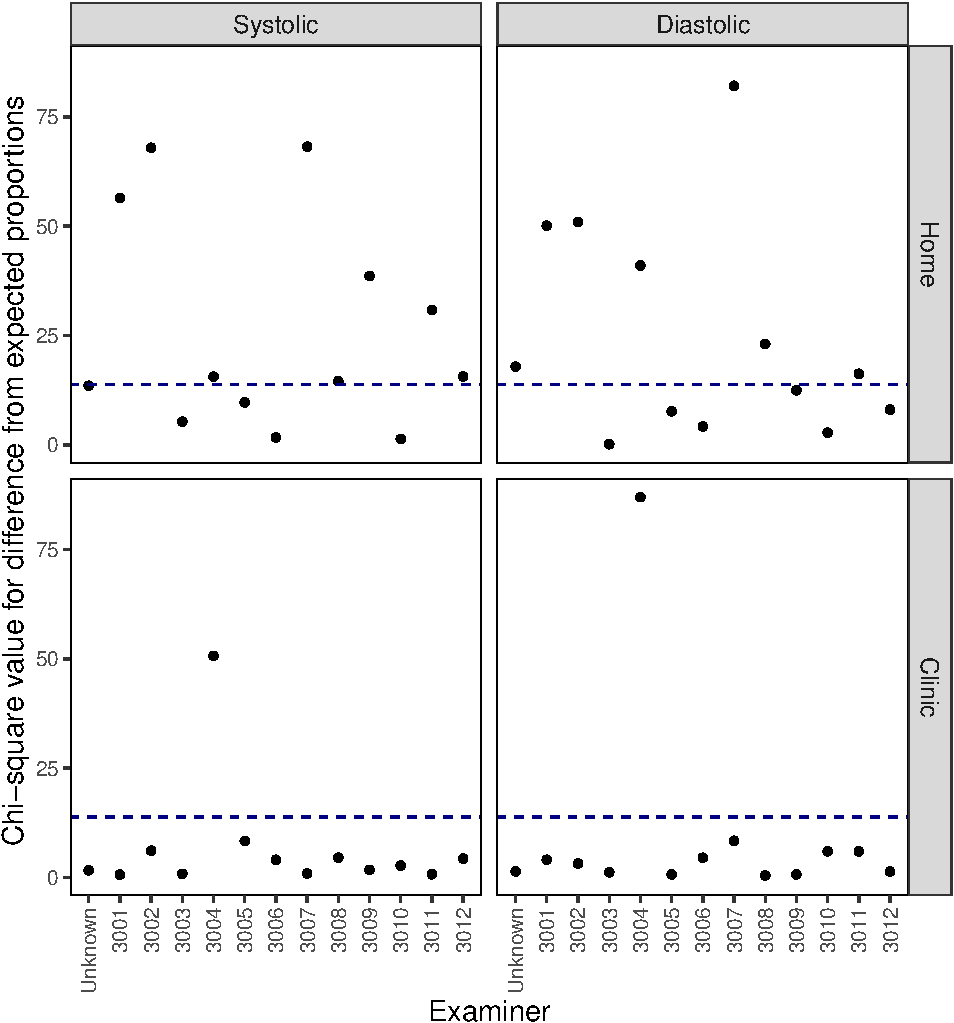
\includegraphics{NHANES-BP-Appendix_files/figure-latex/proportionChisq3-1.pdf}
\caption{\label{fig:proportionChisq3}Proportions of first, second and third measurements from each examiner that are different from the other two, by place and type. Chi-squared value for difference from expected proportions. Dashed line represents p-value 0.001.}
\end{figure}

Given that the position of the differing measure clearly differs from the expected equal proportions, we might ask whether the examiners agree on a common proportion, suggesting that there might be some underlying systematic (observer-independent) reason for the differing measurements.
In Table \ref{tab:ternaryChi2} we show the results of a chi-squared test for equality of observed proportions among the examiners, stratified by place and type.
Interestingly, we see here that the examiners are fairly consistent in their proportions for the Home measures, but not for the Clinic measures.

\begin{table}[!h]

\caption{\label{tab:ternaryChi2}Chi-square test for difference between observed proportions among the examiners, stratified by place and type}
\centering
\begin{tabular}[t]{llrl}
\toprule
Place & Sys/Dias & ChiSq & p-value\\
\midrule
Home & Systolic & 32.8 & 1.69e-01\\
Home & Diastolic & 38.9 & 5.01e-02\\
Clinic & Systolic & 60.0 & 1.67e-04\\
Clinic & Diastolic & 110.0 & 3.05e-12\\
\bottomrule
\end{tabular}
\end{table}

\begin{figure}
\centering
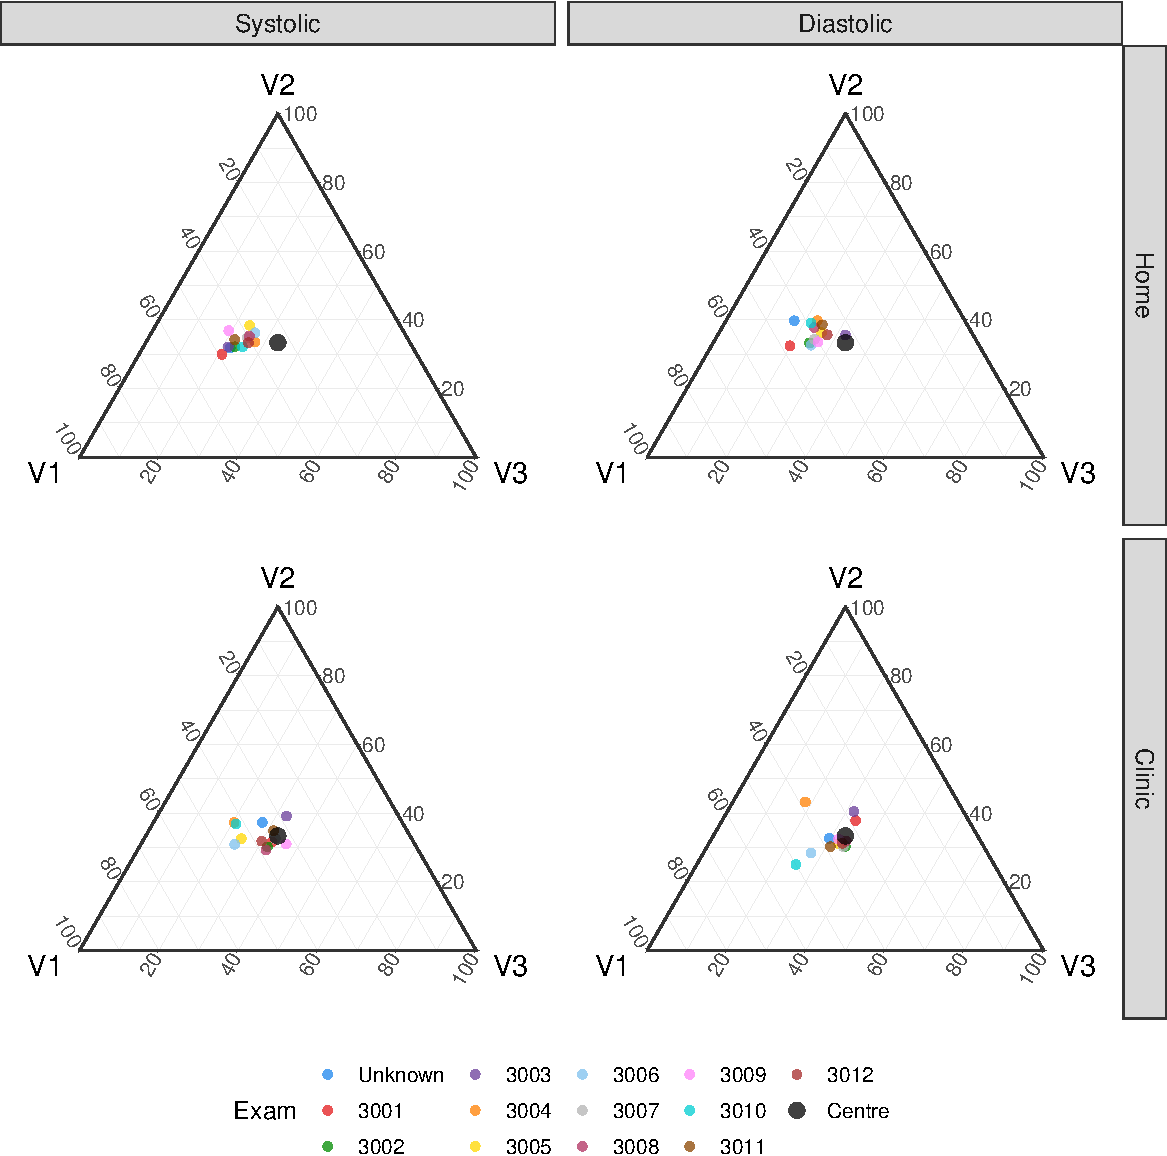
\includegraphics{NHANES-BP-Appendix_files/figure-latex/ternaryPlot-1.pdf}
\caption{\label{fig:ternaryPlot}Ternary plot of the position of the measurement that is unique, among subjects with 2 equal measurements. V1 is the fraction with the first distinct, V2 is the fraction with the second distinct, V3 is the fraction with the third distinct.}
\end{figure}

Looking at a ternary plot Figure \ref{fig:ternaryPlot} for the proportions from the 13 different examiners, we see very clearly the bias toward having the last two measures agree, for almost all examiners, and examiner 3004 (marked larger) standing out as a clear outlier.

Overall, we can only conclude that there are clearly some irregularities in the BP measurement process, but we cannot identify a specific structure to them, or propose a remedy.
As the irregularities are not very large, we will proceed with the analysis without attempting to correct for them.

\hypertarget{sec:BPrange}{%
\subsubsection{Missing or implausible measurements}\label{sec:BPrange}}

Some of the reported measures were extremely implausible, particularly for diastolic BP. NAsubjects had at least one diastolic BP measure recorded as 0, in addition to the 3916 subjects who were missing at least one measurement. We excluded all of these subjects, and indeed any subject who had at least one measurement recorded outside the ranges (40,140) for diastolic and (60,250) for systolic BP, as recommended by the CDC.
There was just one subject with systolic BP measures that were too low, but NA subjects with low diastolic BP (in addition to those with measures recorded as 0).
One subject was excluded for diastolic BP 156, and three were excluded for systolic BP that was too high, with the maximum being 264.

\hypertarget{exploratory-data-analysis}{%
\subsection{Exploratory data analysis}\label{exploratory-data-analysis}}

The empirical means of the home and clinic measures in population B are tabulated in Table 1. We note that the home measures are systematically higher than the clinic measures, within every demographic group, with greater differences for subjects who are white or Mexican, and female.
The average difference is about 2.2 for diastolic and 2.7 for systolic, which is small compared with the general range of the differences, which have SD of
10.5 (diastolic) and 14.8 (systolic).

\begin{table}[!h]

\caption{\label{tab:summaries}Summary data for blood pressure}
\centering
\begin{tabular}[t]{llllrr}
\toprule
Sys/Dias & Place & Sex & Ethnicity & Mean & SD\\
\midrule
Home & Systolic & Male & Black & 128.8 & 2.7\\
Home & Systolic & Male & White & 131.2 & 2.8\\
Home & Systolic & Male & Mexican & 127.1 & 2.5\\
Home & Systolic & Female & Black & 123.2 & 2.7\\
Home & Systolic & Female & White & 127.2 & 2.9\\
Home & Systolic & Female & Mexican & 121.2 & 2.7\\
\addlinespace
Home & Diastolic & Male & Black & 78.7 & 2.4\\
Home & Diastolic & Male & White & 77.1 & 2.3\\
Home & Diastolic & Male & Mexican & 76.8 & 2.4\\
Home & Diastolic & Female & Black & 75.0 & 2.4\\
Home & Diastolic & Female & White & 73.7 & 2.3\\
Home & Diastolic & Female & Mexican & 72.0 & 2.4\\
\addlinespace
Clinic & Systolic & Male & Black & 127.7 & 3.5\\
Clinic & Systolic & Male & White & 128.0 & 4.2\\
Clinic & Systolic & Male & Mexican & 123.5 & 3.5\\
Clinic & Systolic & Female & Black & 122.4 & 3.6\\
Clinic & Systolic & Female & White & 123.5 & 4.1\\
Clinic & Systolic & Female & Mexican & 117.8 & 3.4\\
\addlinespace
Clinic & Diastolic & Male & Black & 77.8 & 3.1\\
Clinic & Diastolic & Male & White & 75.4 & 3.1\\
Clinic & Diastolic & Male & Mexican & 74.9 & 3.2\\
Clinic & Diastolic & Female & Black & 72.4 & 3.0\\
Clinic & Diastolic & Female & White & 70.5 & 3.0\\
Clinic & Diastolic & Female & Mexican & 69.2 & 3.0\\
\bottomrule
\end{tabular}
\end{table}

\hypertarget{sec:correlations}{%
\subsubsection{Correlations between measurements}\label{sec:correlations}}

In Figure \ref{fig:SD-mean} see that there is relatively little correlation between empirical SD and empirical mean SD for the different BP types and places. This is reassuring, as it avoids the possibility of a collinearity effect confounding the sampling of mean and SD, which are being treated as independent covariates in the model.

\begin{figure}
\centering
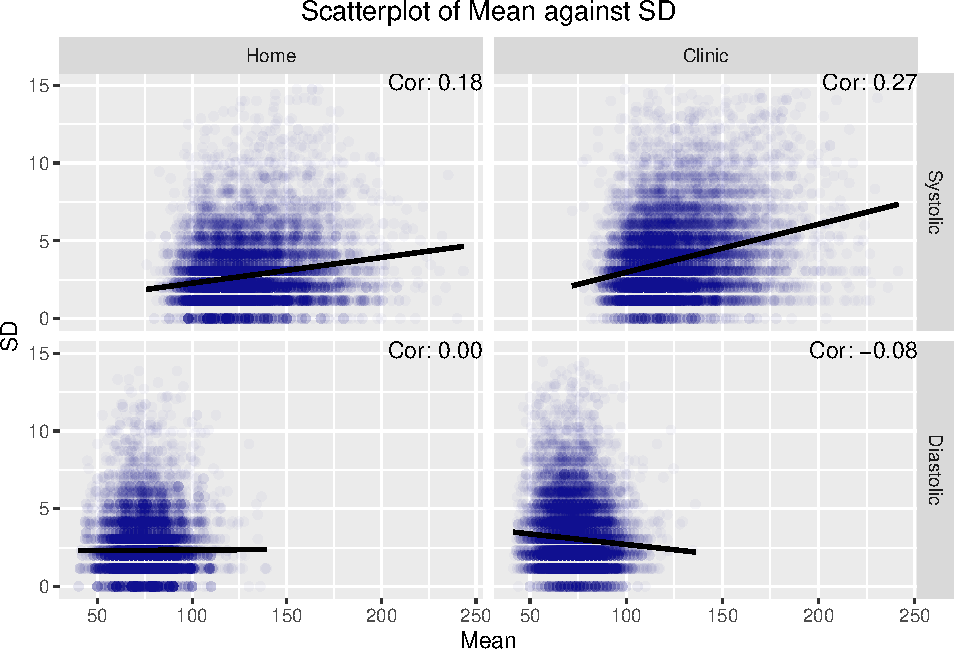
\includegraphics{NHANES-BP-Appendix_files/figure-latex/SD-mean-1.pdf}
\caption{\label{fig:SD-mean}Scatterplot of individual mean BP against individual SD of BP}
\end{figure}

\#```\{r Delta-mean,fig.pos=`H', fig.cap=`Scatterplot of individual mean BP against individual absolute difference between Clinic and Home mean', echo=FALSE,results=`asis',message=FALSE,warning=FALSE\}
\#bp.sub \textless- data.frame(Mean=bp.data\(TotalMean[bp.data\)BPplace==`Clinic'{]},Delta=bp.data\(Delta[bp.data\)BPplace==`Clinic'{]}, \#BPtype=bp.data\(BPtype[bp.data\)BPplace==`Clinic'{]}) \%\textgreater\% \# Home and clinic are identical
\# group\_by(BPtype)

\hypertarget{bp.data.cor---bp.sub}{%
\section{bp.data.cor \textless- bp.sub \%\textgreater\%}\label{bp.data.cor---bp.sub}}

\hypertarget{summarizecorrelationdelta-cormean-delta-use-complete.obs}{%
\section{summarize(correlationDelta = cor(Mean, Delta, use = ``complete.obs''))}\label{summarizecorrelationdelta-cormean-delta-use-complete.obs}}

\hypertarget{scatterplot-of-mean-bp-against-sd-of-bp-from-bp.data}{%
\section{\# Scatterplot of mean BP against SD of BP from bp.data}\label{scatterplot-of-mean-bp-against-sd-of-bp-from-bp.data}}

\hypertarget{ggplotbp.sub-group_bybptype-aesx-mean-y-delta}{%
\section{ggplot(bp.sub \%\textgreater\% group\_by(BPtype), aes(x = Mean, y = Delta)) +}\label{ggplotbp.sub-group_bybptype-aesx-mean-y-delta}}

\hypertarget{geom_pointalpha.03-color-navyblue}{%
\section{geom\_point(alpha=.03, color = `navyblue' ) +}\label{geom_pointalpha.03-color-navyblue}}

\hypertarget{labstitle-scatterplot-of-mean-against-delta}{%
\section{\texorpdfstring{labs(title = ``Scatterplot of Mean against \textbar Delta\textbar{}'',}{labs(title = ``Scatterplot of Mean against \textbar Delta\textbar'',}}\label{labstitle-scatterplot-of-mean-against-delta}}

\hypertarget{x-meany-delta-ylim020}{%
\section{\texorpdfstring{x = ``Mean'',y = ``\textbar Delta\textbar{}'') + ylim(0,20)+}{x = ``Mean'',y = ``\textbar Delta\textbar'') + ylim(0,20)+}}\label{x-meany-delta-ylim020}}

\hypertarget{geom_smoothmethod-lm-se-false-color-black-add-regression-line}{%
\section{geom\_smooth(method = ``lm'', se = FALSE, color = ``black'') + \# Add regression line}\label{geom_smoothmethod-lm-se-false-color-black-add-regression-line}}

\hypertarget{facet_grid-bptype-scales-free_x}{%
\section{facet\_grid(\textasciitilde{} BPtype, scales = `free\_x') +}\label{facet_grid-bptype-scales-free_x}}

\hypertarget{themeplot.title-element_texthjust-0.5}{%
\section{theme(plot.title = element\_text(hjust = 0.5)) +}\label{themeplot.title-element_texthjust-0.5}}

\hypertarget{geom_textdata-bp.data.cor2-aeslabel-sprintfcor-.2f-correlationdelta-x-inf-y-inf}{%
\section{geom\_text(data = bp.data.cor2, aes(label = sprintf(``Cor: \%.2f'', correlationDelta), x = Inf, y = Inf),}\label{geom_textdata-bp.data.cor2-aeslabel-sprintfcor-.2f-correlationdelta-x-inf-y-inf}}

\hypertarget{vjust-top-hjust-right-inherit.aes-false}{%
\section{vjust = ``top'', hjust = ``right'', inherit.aes = FALSE)}\label{vjust-top-hjust-right-inherit.aes-false}}

\begin{table}[!h]

\caption{\label{tab:Delta-mean}Correlation between mean and Delta. Rows correspond to type of Delta, columns to type of mean.}
\centering
\begin{tabular}[t]{lrr}
\toprule
  & SysMean & DiasMean\\
\midrule
SysDelta & 0.137 & 0.014\\
DiasDelta & 0.347 & 0.128\\
\bottomrule
\end{tabular}
\end{table}

In Table \ref{tab:Delta-Mean} we show the correlations between overall mean and absolute difference (\(|\Delta|\)) between clinic and home measurements.
The results are given as a \(2\times2\) table, showing correlations within systolic and diastolic BP, and between the two.
The only moderately high correlation is between Systolic mean and Diastolic absolute Delta, which would correspond to a Variance Inflation Factor of 1.14.
While this is not directly relevant to the present Bayesian methodology, it suggests that this correlation should not substantially affect the estimation of the model coefficients.

\newpage

\hypertarget{appendix-b-model-details}{%
\section{Appendix B -- Model details}\label{appendix-b-model-details}}

This appendix aims to add more detail about the numerical modelling than was provided in the article. This is to ensure that the research methods are transparent and entirely reproducible. The numerical modelling presented in this paper was performed using R combined with Rstan. More detail will be provided here about the model, about the specific methodology used to parameterize the model, and more results are provided that were not included in the main text.

The model used in this research is built from the theory of joint modelling of longitudinal and time-to-event data. This will be described in detail later on in this section, however, in brief, this allows the simultaneous modelling of both longitudinal observation data (in this article, this is blood pressure measurements) and also the time-to-event outcome.
In this research the event of interest is either death from any cause, or death from specifically heart attack, cardiovascular disease (CVD) or cerebrovascular disease (CeVD). We henceforth will refer to this latter mortality as HA-CVD-CeVD.
In the latter case, death from a different cause is treated as a noninformative censoring event.

\hypertarget{survival-analysis-time-to-event}{%
\subsubsection{Survival Analysis (Time-to-Event)}\label{survival-analysis-time-to-event}}

The basic survival model is a Gompertz hazard rate with proportional hazards influences of the blood pressure covariates.
The Gompertz equation
\begin{equation}\label{gompertz}
h_0(t)=B\exp{\left(\theta(x+T)\right)},
\end{equation}
describes the baseline hazard of the population to a particular risk, which, for this article, investigates HA-CVD-CeVD mortality specifically, as well as studying mortality risk in general. \(x\in\mathbb{N^N}\) is the age of the individual at the initial interview time, for \(N\) the number of individuals, and \(T\in\mathbb{R}^{+,N}\) the time since the individual entered the survey.
Note that both \(B\) and \(\theta\) have 6 different values, depending on the sex reported at the initial interview -- female or male --- or the race --- black, white or `other'.
Note that `other' in the race category is a combination of all non-black or non-white racial identities, such as Hispanic populations.
The log-linear proportional hazards model links the covariates of the model (mean systolic blood pressure, variance in the diastolic blood pressure, etc) to the survival outcome of the individual via the equation
\begin{equation}\label{prophaz}
h(t)=h_0(t)\exp{\left(\boldsymbol{\beta}\cdot(\boldsymbol{X}-\hat{\boldsymbol{X}})\right)},
\end{equation}
where \(\boldsymbol{X}\in\mathbb{R}^{+,N\times d}\) is a vector of summary statistics of the blood pressure measurements of individual covariates in our model, \(\hat{\boldsymbol{X}}\in\mathbb{R}^{+,d}\) is the centering of the covariates such that the equation \(\sum_i^N \exp{(\boldsymbol{\beta}\cdot(\boldsymbol{X}-\hat{\boldsymbol{X}}))}=0\) is approximately satisfied (more on this later), and \(\boldsymbol{\beta}\in\mathbb{R}^d\) implies the strength of the influence of the covariate on the mortality risk.
The majority of mortality events are censored --- not yet known at the time of data collection --- the censoring indicator being notated as \(\delta\in \{0,1\}\).
When HA-CVD-CeVD mortality is the event being analysed, deaths due to other causes are treated as noninformative censoring events.
In this study, we explored the following covariates:

\begin{tabular}{lll}
\toprule
Variable Name & Support & Description\\
\midrule
$FRS-1998$ & $R^N$ & 1998 version of the FRS score\\
$FRS-ATP$ & $R^N$ & ATP version of the FRS score\\
$M_S$ & $R^{+,N}$ & Mean systolic blood pressure\\
$M_D$ & $R^{+,N}$ & Mean diastolic blood pressure\\
$\Delta_S$ & $R^{+,N}$ & Semi-difference between Home and Clinic mean systolic blood pressure\\
\addlinespace
$\Delta_D$ & $R^{+,N}$ & Semi-difference between Home and Clinic mean diastolic blood pressure\\
$\sigma_{\{S,H\}}$ & $R^{+,N}$ & Standard deviation of the systolic blood pressure taken at home\\
$\sigma_{\{D,H\}}$ & $R^{+,N}$ & Standard deviation of the diastolic blood pressure taken at home\\
$\sigma_{\{S,C\}}$ & $R^{+,N}$ & Standard deviation of the systolic blood pressure taken at the clinic\\
$\sigma_{\{D,C\}}$ & $R^{+,N}$ & Standard deviation of the diastolic blood pressure taken at the clinic\\
\addlinespace
$\tau_{\{S,H\}}$ & $R^{+,N}$ & Precision of the systolic blood pressure taken at home\\
$\tau_{\{D,H\}}$ & $R^{+,N}$ & Precision of the diastolic blood pressure taken at home\\
$\tau_{\{S,C\}}$ & $R^{+,N}$ & Precision of the systolic blood pressure taken at the clinic\\
$\tau_{\{D,C\}}$ & $R^{+,N}$ & Precision of the diastolic blood pressure taken at the clinic\\
\bottomrule
\end{tabular}

Please note that the last four elements of this list, the precision values, were only carried out to ensure model consistency with the use of standard deviation instead.
Note as well that the \(\Delta\) covariates, representing the medium-term variability, enter into the log relative risk sum as an \textbf{absolute value}.

For the parametrization of this model, we assume that the Gompertz parameters and the parameters in the linear predictor term are distributed as follows:
\begin{equation}\label{priorsS}
\begin{aligned}
  \boldsymbol{B}\sim\mathbb{C}(\mu_B,\sigma_B),\\
  \boldsymbol{\theta}\sim\mathcal{N}(\mu_\theta,\sigma_\theta),\\
  \boldsymbol{\beta}\sim \mathcal{N}(\mu_\beta,\sigma_\beta),
\end{aligned}
\end{equation}
noting that \(\mathbb{C}(\mu,\sigma)\) is the Cauchy distribution.

The likelihood for this Gompertz proportional hazards model, over all individuals in the census, is as follows:
\begin{equation}\label{likesurv}
L_S(\boldsymbol{v},\boldsymbol{\delta})=\prod_i^N f(v_i,\delta_i|B_i,\theta_i,\beta_i,\boldsymbol{X},\hat{\boldsymbol{X}})=\prod_i^N h(v_i|B_i,\theta_i,\beta_i,\boldsymbol{X},\hat{\boldsymbol{X}})^{\delta_i} \exp{\left( -\sum_i^N H(v_i|B_i,\theta_i,\beta_i,\boldsymbol{X},\hat{\boldsymbol{X}}) \right)},
\end{equation}
with \(H(v)=\int_0^v h(w)dw\) the cumulative hazard.

\hypertarget{longitudinal-modelling}{%
\subsubsection{Longitudinal Modelling}\label{longitudinal-modelling}}

The mortality hazard rates are assumed to be influenced by individual-level blood pressure means and variability characteristics.
These characteristics are not directly observed, but are inferred from their influence on the individual blood pressure measurements, which have been observed.
Let \(Y_i(t_j)\) be the observed blood pressure for patient \(i\) at time \(t_j\), for the individual \(i\in 1,2,...,N\) and the number of blood pressure measurements per individual \(j\in 1,2,...,k\). Due to the fact that the blood pressure measurement data was taken at both the home and clinic (written using subscripts H and C, respectively), with approximately 6 months between these two measurements, we model the blood pressure using the following model, assuming the diastolic \(Y_{i}^D\) and systolic \(Y_{i}^S\) blood pressure to be Gaussian-distributed:
\begin{equation}\label{bp}
\begin{aligned}
  (Y_{i}^D)_{H} \sim \mathcal{N}(M_i^D+\Delta_i^D,(\sigma_i^D)_H),\\
  (Y_{i}^D)_{C} \sim \mathcal{N}(M_i^D-\Delta_i^D,(\sigma_i^D)_C),\\
  (Y_{i}^S)_{H} \sim \mathcal{N}(M_i^S+\Delta_i^S,(\sigma_i^S)_H),\\
  (Y_{i}^S)_{C} \sim \mathcal{N}(M_i^S-\Delta_i^S,(\sigma_i^S)_C),
\end{aligned}
\end{equation}
where superscripts \(D\) and \(S\) refer to diastolic and systolic blood pressure, respectively.

The blood pressure characteristics --- the individual-level parameters --- are themselves distributed according to a hierarchical model, determined by population-level parameters (also called ``hyperparameters'\,'):
\begin{equation}\label{priorsL}
\begin{aligned}
  M_i^{\{D,S\}}\sim \mathcal{N}(\mu_M^{\{D,S\}},\sigma_M^{\{D,S\}}),\\
  \Delta_i^{\{D,S\}}\sim \mathcal{N}(\mu_D^{\{D,S\}},\sigma_D^{\{D,S\}}),\\
  \sigma_{i,C}^{\{D,S\}}\sim \Gamma(r_C^{\{D,S\}},\lambda_C^{\{D,S\}}),\\
  \sigma_{i,H}^{\{D,S\}}\sim \Gamma(r_H^{\{D,S\}},\lambda_H^{\{D,S\}}).
\end{aligned}
\end{equation}
The longitudinal outcome modelling therefore aims to infer these hyperparameters
\begin{equation}
  \Theta=\left\{\mu_M^{\{D,S\}},\mu_D^{\{D,S\}},\sigma_M^{\{D,S\}},\sigma_D^{\{D,S\}},r_C^{\{D,S\}},\lambda_C^{\{D,S\}},r_H^{\{D,S\}},\lambda_H^{\{D,S\}}\right\},
\end{equation}
and to use the implied uncertainty about the individual-level parameters to inform the inference about the survival parameters.
The likelihood for the longitudinal measurements is therefore (combining the systolic and diastolic into a single parameter for simplicity):
\begin{equation}\label{likelong}
  L_L(\Theta|Y)=\prod_{i=1}^N\left(\prod_{j=1}^{k}f(y_{ij}|M_i,\Delta_i,\sigma_i)\right)f(M_i|\mu_M,\sigma_M)f(\Delta_i|\mu_D,\sigma_D)f(\tau_{i,C}|r_C,\lambda_C)f(\tau_{i,H}|r_H,\lambda_H)
\end{equation}

\hypertarget{combined-hierarchical-model}{%
\subsubsection{Combined Hierarchical Model}\label{combined-hierarchical-model}}

Combining the longitudinal outcome and time-to-event partial likelihoods, and for a given parameter space value of \(\Omega=\{\beta,B,\theta\}\cup \Theta\), the joint likelihood is
\begin{equation}
\begin{split}
  L(\Omega|Y)=\prod_{i=1}^N\left(\prod_{j=1}^{k}f(y_{ij}|M_i,\Delta_i,\sigma_i)\right)f&(v_i,\delta_i|B_i,\theta_i,\beta_i,\boldsymbol{X},\hat{\boldsymbol{X}})f(M_i|\mu_M,\sigma_M)\\
  &f(\Delta_i|\mu_D,\sigma_D)f(\tau_{i,C}|r_C,\lambda_C)f(\tau_{i,H}|r_H,\lambda_H).
  \end{split}
\end{equation}
One approach to estimating the complete set of hyperparameters
\begin{equation}
  \Omega_H=\{\mu_B,\sigma_B,\mu_\theta,\sigma_\theta,\mu_\beta,\sigma_\beta,\mu_M^{\{D,S\}},\sigma_M^{\{D,S\}},\mu_D^{\{D,S\}},\sigma_D^{\{D,S\}},r_C^{\{D,S\}},\lambda_C^{\{D,S\}},r_H^{\{D,S\}},\lambda_H^{\{D,S\}}\}
\end{equation}
is to impose a higher-level prior distribution, and use the machinery of Bayesian inference to produce posteriors for everything.
This approach runs into computational difficulties, which have led us to a two-stage `empirical Bayes' approach, where the hyperparameters for the longitudinal model are first fixed by a maximum-likelihood calculation, after which the remaining hyperparameters and individual-level parameters can be estimated with Bayesian machinery.
For the time-to-event parameters we choose flat hyperpriors, selecting the hyperparameters \(\mu_B=\mu_\theta=\mu_\beta=0\), \(\sigma_B=\sigma_\theta=2\), and \(\sigma_\beta=100\).

\hypertarget{the-modelling-variants}{%
\subsubsection{The modelling variants}\label{the-modelling-variants}}

In this article, we researched into 16 variants of the model-fitting problem, but focussed mainly on 8 of them.
The 8 main models use the standard deviation, \(\sigma\), as the measure of the influence of blood-pressure variability on mortality.
We also produced the same 8 models but using precision, \(\tau=1/\sigma^2\), as the measure of the influence of blood-pressure variability on mortality.
However, this was only to ensure that there were no differences between the use of one over the other.
Throughout the remainder of this appendix, we refer to the 8 main models using the following run numbers:

\begin{enumerate}
\item All participants (14,654), using mean systolic and diastolic blood pressure (not FRS) in the linear predictor term, with the outcome data as death specifically from HA-CVD-CeVD.
\item All participants (14,654), using mean systolic and diastolic blood pressure (not FRS) in the linear predictor term, with the outcome data as all-causes of death.
\item Only participants that had data from which FRS values could be computed (N=9,008) --- the ``FRS population'' but using mean systolic and diastolic blood pressure (not FRS) in the linear predictor term, with the outcome data as death specifically from HA-CVD-CeVD.
\item FRS population, but using mean systolic and diastolic blood pressure (not FRS) in the linear predictor term, with the outcome data as all-causes of death.
\item FRS population, and using the FRS ATP-III value in the linear predictor term, with the outcome data as death specifically from HA-CVD-CeVD.
\item FRS population, and using the FRS ATP-III value in the linear predictor term, with the outcome data as all-causes of death.
\item FRS population, and using the FRS 1998-version value in the linear predictor term, with the outcome data as death specifically from HA-CVD-CeVD.
\item FRS population, and using the FRS 1998-version value in the linear predictor term, with the outcome data as all-causes of death.
\label{tab:runnums}
\end{enumerate}

We also include Directed Acyclical Graph (DAG) sketches to help visualize the different models, as shown in figures \ref{fig:DAGmean} and \ref{fig:DAGFRS}.
In order to read the DAGs, note that each square background layer that appears as a stack of layers represents different measured outcomes that were made in the first wave of the survey.
The outcome variables measured are represented by a square-shaped text box, and a parameter of the model is represented by a circular-shaped text box. If either a square or circular text box is placed on top of a stacked rectangular layer, it means that multiple values of that variable (as many as there are layers to the stack) are either measured (for outcome variables) or simulated (for parameters of the model). Please note that the number of layers in the stack is written in the text box that does not contain a frame which is intentionally displayed on top of the stacked layer that it represents. For example, \(i=1,...,N\).
Finally, the direction of the arrows implies causality assumed in the model.

\begin{figure}
\hypertarget{fig:DAGmean}{%
\centering
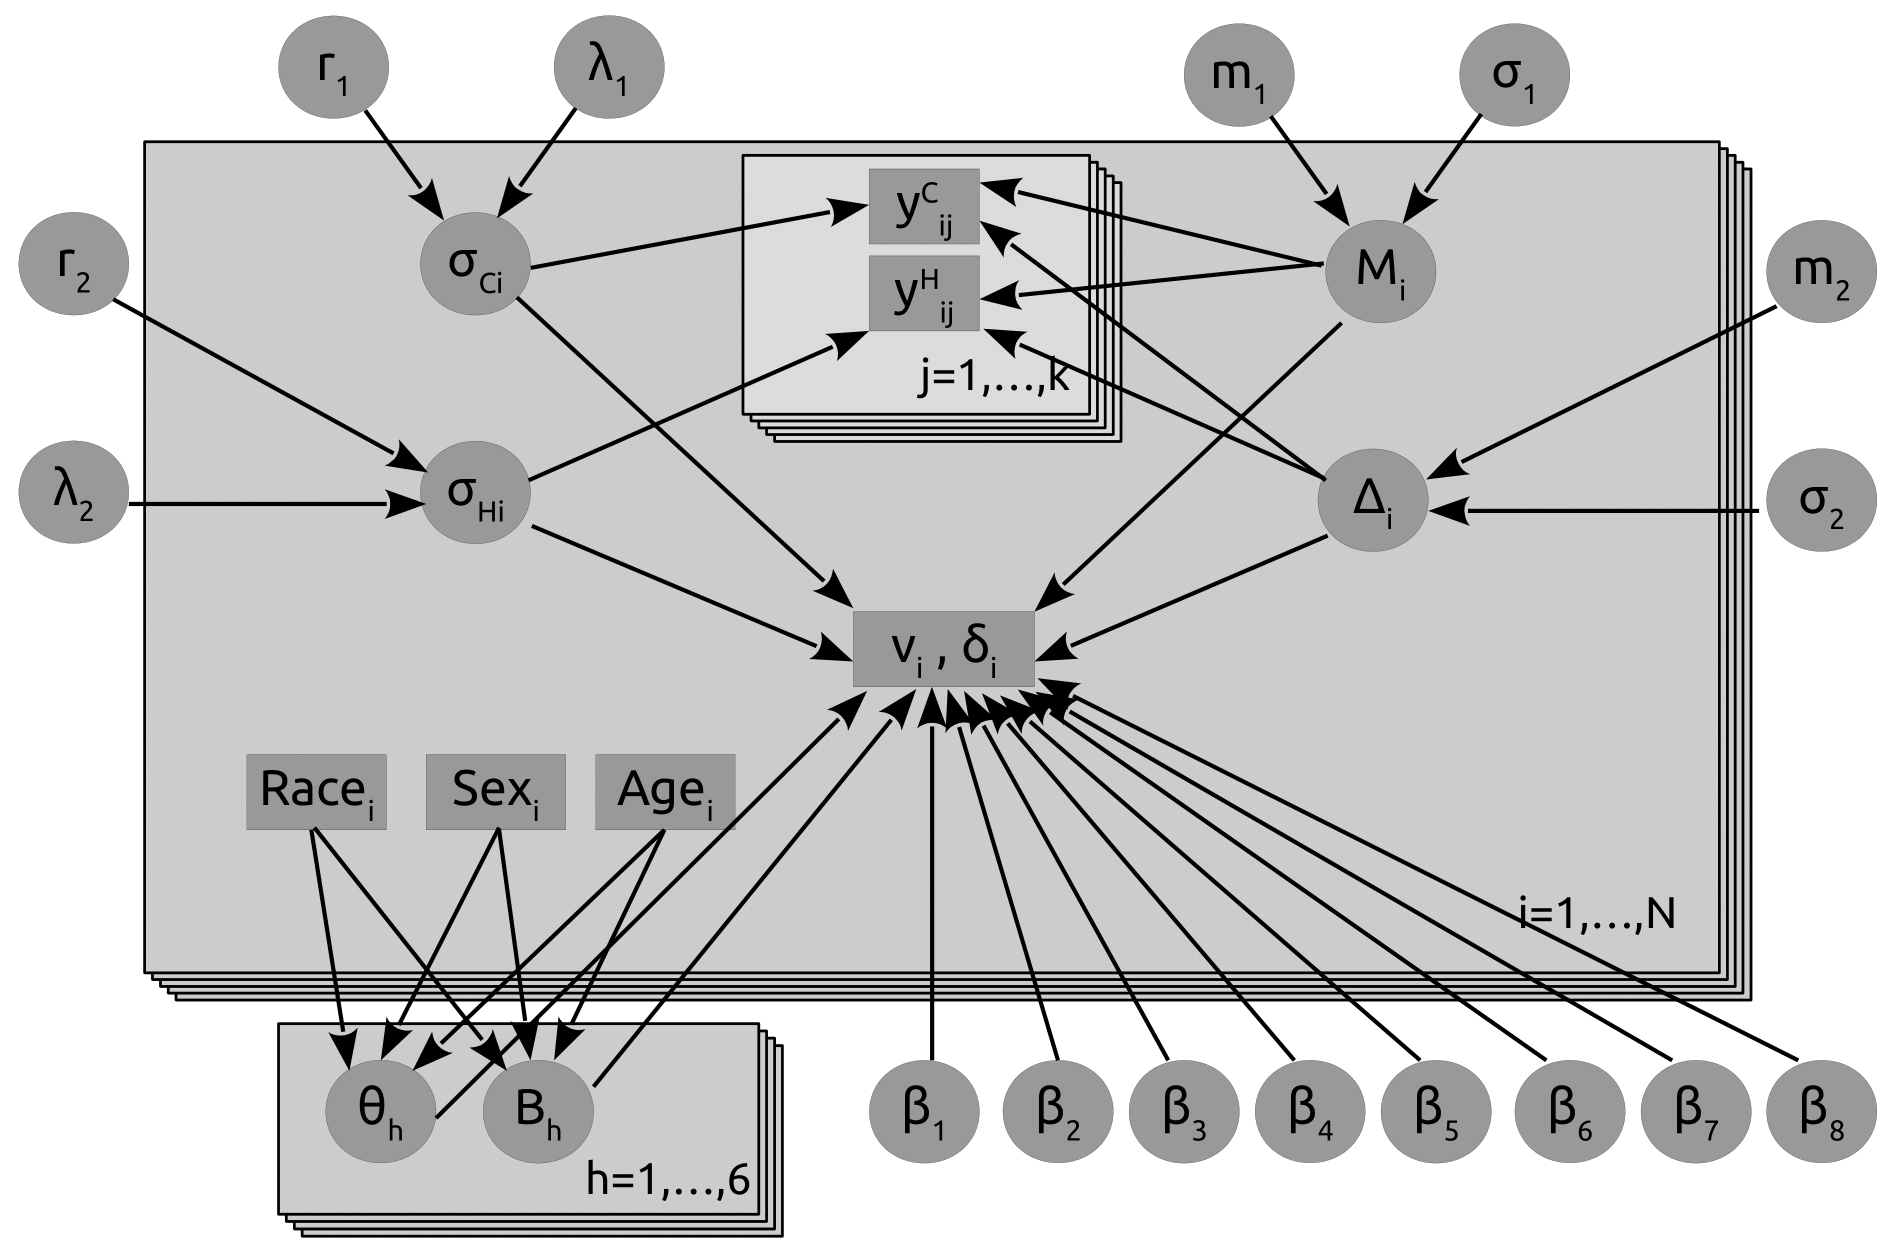
\includegraphics{./DAG_Mean.png}
\caption{An illustration of the DAG of the mean blood pressure-based model presented in this article.}\label{fig:DAGmean}
}
\end{figure}

\begin{figure}
\hypertarget{fig:DAGFRS}{%
\centering
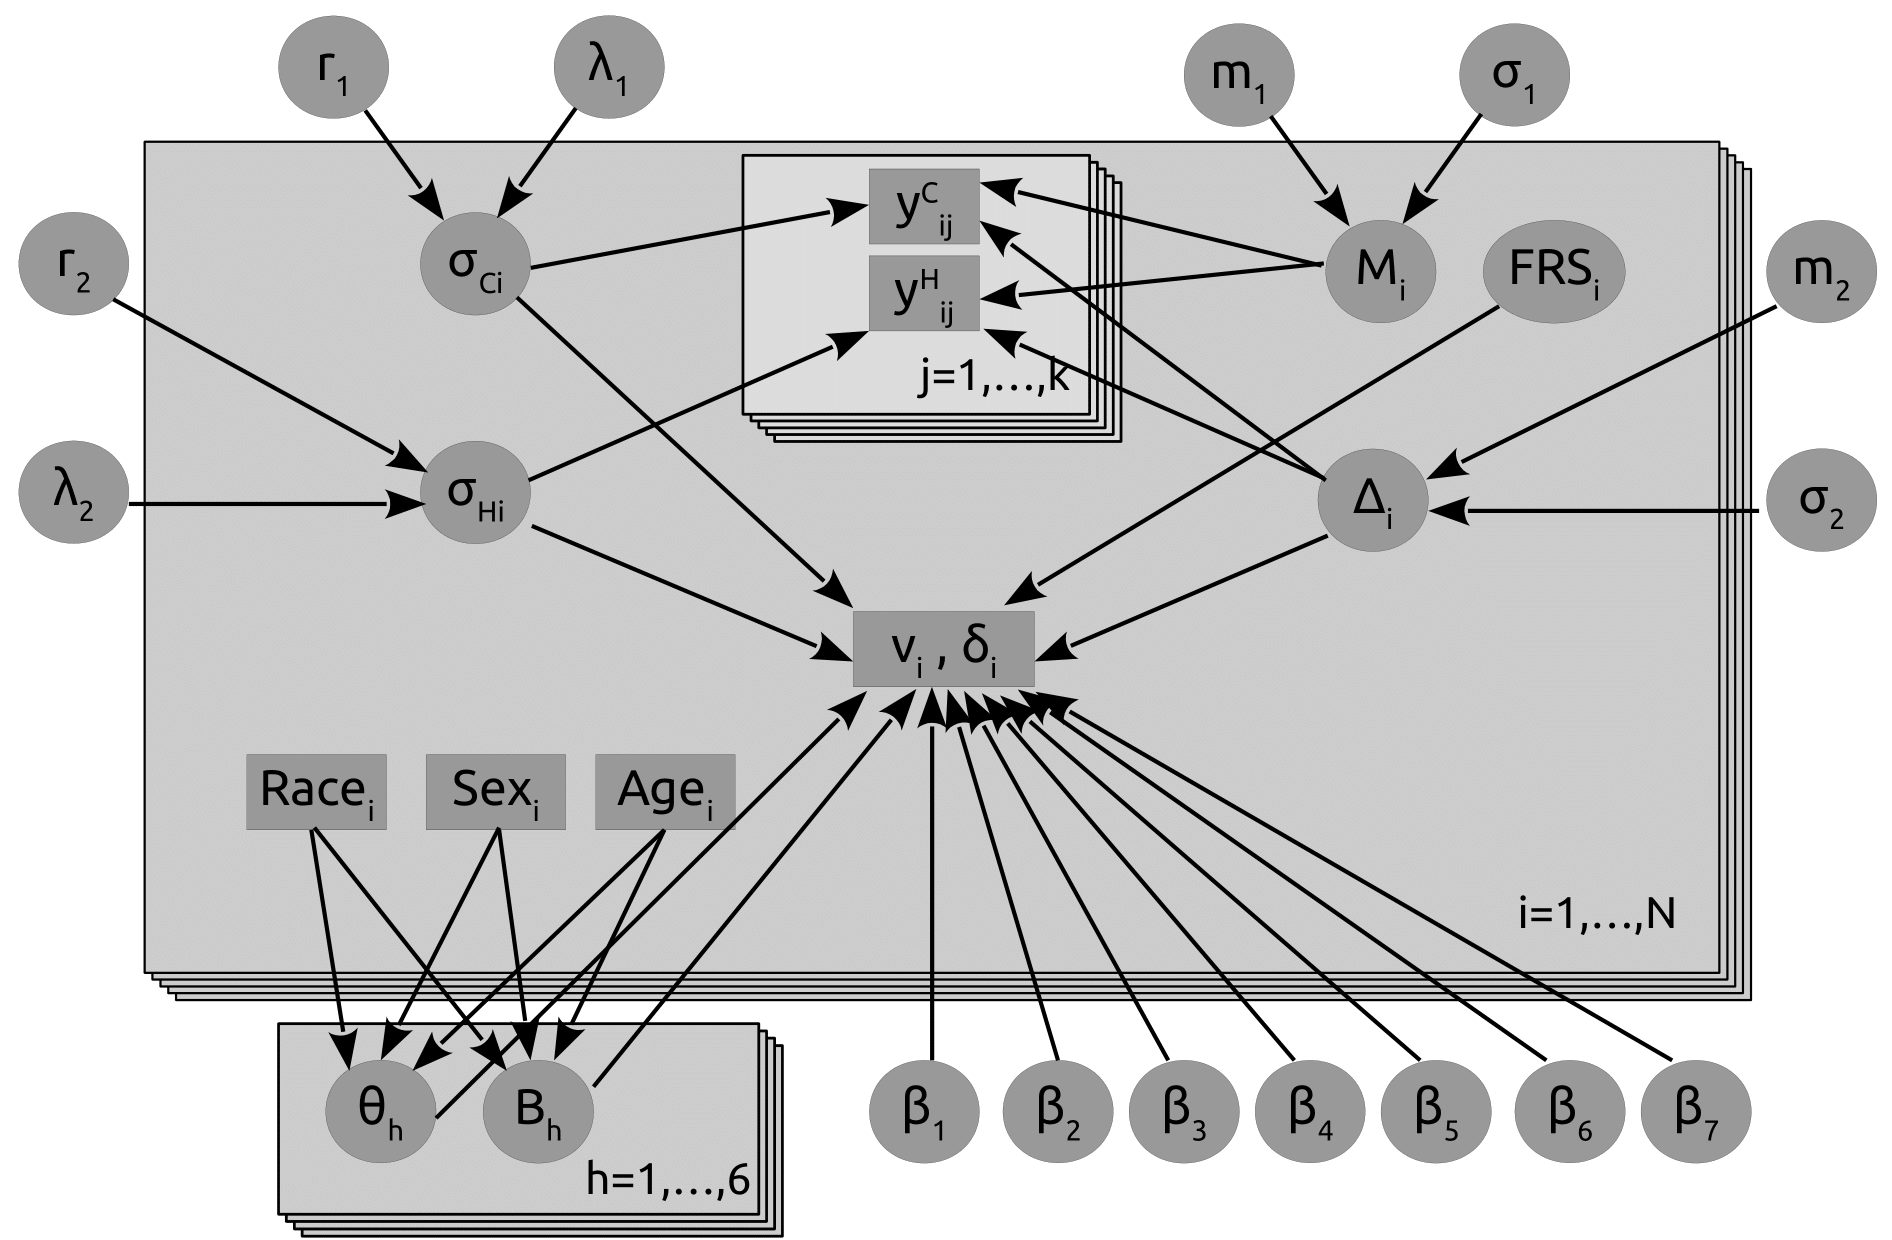
\includegraphics{./DAG_FRS.png}
\caption{An illustration of the DAG of the FRS-based model presented in this article.}\label{fig:DAGFRS}
}
\end{figure}

For convenience, we provide an overview of the different blood pressure values in the full and FRS populations in tables \ref{tab:BloodFull} and \ref{tab:BloodFRS}.

\begin{table}

\caption{\label{tab:BloodFull}Parameters for distribution of blood pressure, for the full population}
\centering
\begin{tabular}[t]{llrr}
\toprule
BP & Variable & Mean & SD\\
\midrule
Systolic & Overall Mean & 125.36 & 19.48\\
Systolic & Delta & 5.24 & 4.86\\
Systolic & Home SD & 2.74 & 2.05\\
Systolic & Clinic SD & 3.78 & 2.61\\
Diastolic & Overall Mean & 74.34 & 10.29\\
\addlinespace
Diastolic & Delta & 3.90 & 3.14\\
Diastolic & Home SD & 2.34 & 1.75\\
Diastolic & Clinic SD & 3.08 & 2.08\\
\bottomrule
\end{tabular}
\end{table}

\begin{table}

\caption{\label{tab:BloodFRS}Parameters for distribution of blood pressure, for the FRS population}
\centering
\begin{tabular}[t]{llrr}
\toprule
BP & Variable & Mean & SD\\
\midrule
Systolic & Overall Mean & 125.89 & 18.33\\
Systolic & Delta & 5.23 & 4.71\\
Systolic & Home SD & 2.78 & 2.06\\
Systolic & Clinic SD & 3.78 & 2.52\\
Diastolic & Overall Mean & 76.41 & 10.00\\
\addlinespace
Diastolic & Delta & 3.84 & 3.10\\
Diastolic & Home SD & 2.28 & 1.71\\
Diastolic & Clinic SD & 2.92 & 1.97\\
\bottomrule
\end{tabular}
\end{table}

\hypertarget{methodology}{%
\subsection{Methodology}\label{methodology}}

The methodology for this research can be split into three main sections: 1) calculating the empirical Bayes' parameters, 2) parameterizing the model using Hamiltonian Monte Carlo (HMC) and 3) re-centering the variables in the linear predictor equation. By applying empirical Bayes', Maximum Likelihood Estimates (MLEs) of some of the parameter distributions are provided. Note that the parameters estimated here are only the prior distribution of the global (not individual) blood pressure means and the variances, for both systolic and diastolic and home and clinic measurements. These estimates are then provided as prior distributions for the Stan MCMC simulations using HMC, where estimates can be made for all the parameter distributions of the model, given the specific centering applied. Finally, section (3) recalculates the centering values based on the previous MCMC iteration, and sets of the next iteration, while simultaneously checking for convergence in both the MCMC simulations and the centering values.

\hypertarget{empirical-bayes-parameters}{%
\subsubsection{Empirical Bayes Parameters}\label{empirical-bayes-parameters}}

First, we extract the intervals for the digits in the blood pressure measurement recordings. Suppose the fractions of digits 0,2,4,6,8 are \(b_0,b_2,b_4,b_6,b_8\).
Letting \(B_0=0\) and \(B_k=10\sum_{j=0}^{k-1}b_{2j}\) for \(k=1,\dots,5\),
we want to choose a positive \(a\) and place breaks at \(-a+B_k\), so that measurements between \(-a+B_k\) and \(-a+B_{k+1}\) modulo
10 are assigned the final digit \(2k\), for \(k=0,\dots,4\).
We choose \(a\) to minimise the total distance of the intervals from the rounded value:
\[
  \sum_{k=0}^4 \int_{-a+B_k}^{-a+B_{k+1}} \bigl| x-2k\bigr|\mathrm{d} x=\frac12\sum_{k=0}^4 \left(-a+B_k-2k\right)^2 + \left(-a+B_{k+1}-2k\right)^2,
\]
as long as \(2k\) is in the appropriate interval. This is minimized at
\[
  a= \frac{1}{5}\left(B_1+B_2+B_3+B_4 - 15\right)=\sum_{j=0}^3 (8-2j) b_{2j} \, - 3.
\]

Next step, we fit the BP distribution parameters. We suppose that each individual has BP measures
\(\tilde{y}_{ij}^l\) for \(i=1,\dots,n\), \(j=1,\dots,k\) (default \(k=3\)),
and \(l=1,2\), which are rounded versions of
\[
  y_{ij}^l \sim \mathcal{N}\bigl( \mu_i^l,(\tau_i^l)^{-1}\bigr),
\]
where
\begin{align*}
\mu_i^1&=(M_i+\Delta_i)/2,\\
\mu_i^2&=(M_i-\Delta_i)/2,\\
M_i&\sim \mathcal{N}\bigl(m_M,\sigma^2_M) \text{ and }
  \Delta_i\sim \mathcal{N}\bigl(m_\Delta,\sigma^2_\Delta) \text{ independent,}\\
  \tau_i^l &\sim \mathrm{Gamma}(\alpha^l,\alpha^l/\theta^l ).
\end{align*}
(Note that \(\alpha^l\) is the usual shape parameter,
while \(\theta^l\) is the expectation.)

We wish to estimate the eight parameters
\[
(m_M,m_\Delta,\sigma^2_M,\sigma^2_\Delta,\alpha^1,\theta^1,\alpha^2,\theta^2)
\]
We begin by assuming \(y_{ij}^l\) observed directly. We estimate
by maximising the partial likelihood on the observations
\begin{align*}
  \bar{y}_{i+}&:= \frac{1}{2k} \sum_{j=1}^k y_{ij}^1 + y_{ij}^2,\\
  \bar{y}_{i-}&:= \frac{1}{2k} \sum_{j=1}^k y_{ij}^1 - y_{ij}^2,\\
  s_i^l&:=  \frac{1}{k-1}\sum_{j=1}^k \Bigl( y_{ij}^l - \frac{1}{k} \sum_{j=1}^k y_{ij}^l \Bigr)^2.
\end{align*}
Note that
\[
(k-1)s_i^l \tau_i^l =\sum_{j=1}^k \Bigl( z_{ij}^l - \frac{1}{k} \sum_{j=1}^k z_{ij}^l \Bigr)^2.
\]
where \(z_{ij}^l\) are i.i.d.~standard normal
is independent of \(\tau_i^l\), thus has a chi-squared distribution
with \(k-1\) degrees of freedom --- hence \(\frac{k-1}{2}\cdot s_i^l\tau_i^l\) is
gamma distributed with parameters \((\frac{k-1}{2},1)\). Since \(\frac{\alpha}{\theta}\tau_i^l\) is independent of \(s_i^l\tau_i^l\), with \(\mathrm{Gamma}(\alpha,1)\) distribution, we see that \(\frac{\theta(k-1)}{2\alpha}s_i^l\) is the ratio of two independent gamma random variables, hence has beta-prime distribution with parameters \(\left(\frac{k-1}{2}, \alpha \right)\), so log partial likelihood
\[
  \ell_{\operatorname{Beta}}(\alpha,\theta;s^l_\cdot)=n\alpha \log\frac{\alpha}{\theta}+n\log\Gamma\left(\alpha+\frac{k-1}{2}\right)-n\log\Gamma(\alpha)
  + \frac{k-1}{2} \sum_{i=1}^n \log s_i^l -\left(\alpha+\frac{k-1}{2}\right) \sum_{i=1}^n \log \left(s_i^l+\frac\alpha\theta\right).
\]
Note as well that these quantities \((k-1)s_i^l\) should correspond to empirically observed individual variances; hence we will compare these empirical variances (with imputed fractional parts) divided by the normalization factor \(2\alpha/(k-1)\theta\) to the beta-prime distribution below as a goodness-of-fit test.

The partial Fisher Information has entries
\begin{align*}
 -\frac{\partial^2 \ell}{\partial \alpha^2} &=
   n\psi_1\left(\alpha\right) - n\psi_1\left(\alpha+\frac{k-1}{2}\right)
  - \frac{n}{\alpha} +\sum_{i=1}^n \frac{2\theta s_i^l + \alpha-(k-1)/2}{(\theta s_i^l + \alpha)^2}\\
-\frac{\partial^2 \ell}{\partial \theta^2} &=
   -\frac{n \alpha}{\theta^2} +\frac{\alpha}{\theta^2}\left(\alpha+\frac{k-1}{2}\right)\sum_{i=1}^n \frac{2\theta s_i^l + \alpha}{(\theta s_i^l + \alpha)^2}\\
-\frac{\partial^2 \ell}{\partial \theta\partial\alpha} &= \frac{n}{\theta}-
   \frac1\theta \sum_{i=1}^n \frac{\alpha^2+2\alpha\theta s_i^l+\frac{k-1}{2}\theta s_i^l}{(\theta s_i^l + \alpha)^2}.
\end{align*}
where \(\psi_1\) is the trigamma function.

Let \((\hat\alpha^l,\hat\beta^l)\) be the maximum partial likelihood estimators. Conditioned on \((\tau_i^l)\) we have
\begin{align*}
  \bar{y}_{i+}&\sim \mathcal{N}\left(m_M, \sigma^2_M + \frac{1}{4k}\left( \frac{1}{\tau_i^1}+\frac{1}{\tau_i^2}\right)\right),\\
  \bar{y}_{i-}&\sim \mathcal{N}\left(m_\Delta,\sigma^2_\Delta + \frac{1}{4k}\left( \frac{1}{\tau_i^1}+\frac{1}{\tau_i^2}\right)\right).
\end{align*}
We would then have MLEs
\begin{align*}
  \hat{m}_M&= \frac{1}{n} \sum_{i=1}^n \bar{y}_{i+},\\
  \hat{m}_\Delta&= \frac{1}{n} \sum_{i=1}^n \bar{y}_{i-},
\end{align*}
which are approximately normally distributed, with means \(m_M\) and \(m_\Delta\) respectively, and conditional on \(\tau_i^l\) standard errors
\[
  \frac{\sigma_M^2}{n}+\frac{1}{4kn^2} \sum_{i=1}^n (\tau_i^1)^{-1} + (\tau_i^2)^{-1} \quad \text{ and } \quad
  \frac{\sigma_\Delta^2}{n}+\frac{1}{4kn^2} \sum_{i=1}^n (\tau_i^1)^{-1} + (\tau_i^2)^{-1},
\]
which we may approximate --- with error on the order of \(n^{-3/2}\) --- replaceing the mean of \((\tau_i^l)^{-1}\) by its expected value \(\beta^l/(\alpha^l-1)\) to obtain
\begin{align*}
  \mathrm{Var}(\hat{m}_M) &\approx \frac{\sigma_M^2}{n}+\frac{1}{4kn}\left( \frac{\beta^1}{\alpha^1-1}+ \frac{\beta^2}{\alpha^2-1}\right) \\
  \mathrm{Var}(\hat{m}_\Delta) &\approx \frac{\sigma_\Delta^2}{n}+\frac{1}{4kn}\left( \frac{\beta^1}{\alpha^1-1}+ \frac{\beta^2}{\alpha^2-1}\right) 
\end{align*}
Finally, conditioned on the \(\tau_i^l\) we have that the random variables \(\bar{y}_{i+}\) are normal with variance
\[
  \sigma_M^2+\frac{1}{4k}\left((\tau_i^1)^{-1} + (\tau_i^1)^{-1} \right),
\]
so the unconditional variance is the expected value, or
\[
  \sigma_M^2+\frac{1}{4k}\left(\frac{\beta^1}{\alpha^1-1}+ \frac{\beta^2}{\alpha^2-1} \right).
\]
This yields the estimators
\begin{align*}
  \hat\sigma_M^2 &=\frac{1}{n-1}\sum_{i=1}^n\left(\bar{y}_{i+}-n^{-1}\sum_{i=1}^n y_{i+}\right)^2 - \frac{1}{4k}\left(\frac{\hat\beta^1}{\hat\alpha^1-1}+ \frac{\hat\beta^2}{\hat\alpha^2-1} \right),\\
  \hat\sigma_\Delta^2 &=\frac{1}{n-1}\sum_{i=1}^n\left(\bar{y}_{i-}-n^{-1}\sum_{i=1}^n y_{i-}\right)^2 - \frac{1}{4k}\left(\frac{\hat\beta^1}{\hat\alpha^1-1}+ \frac{\hat\beta^2}{\hat\alpha^2-1} \right).
\end{align*}
Using the delta method, and the fact that we see that the variance of \(\hat\beta/(\hat\alpha-1)\) is approximately
\[
  \frac{\sigma_\beta^2}{(\hat\alpha-1)^2} + \frac{\hat\beta^2\sigma_\alpha^2}{(\hat\alpha-1)^4},
\]
where \(\sigma_\alpha\) and \(\sigma_\beta\) are the standard errors for \(\hat\alpha\) and \(\hat\beta\) respectively, so the standard errors for \(\hat\sigma_M^2\) and \(\hat\sigma_\Delta^2\) are approximately
\begin{align*}
  \operatorname{SE}\left(\hat\sigma_M^2\right)&\approx \frac{1}{2k}\Bigl(\frac{8k^2\hat\sigma_M^2}{n} + \frac{\sigma_\beta^2}{(\hat\alpha^1-1)^2} + \frac{(\hat\beta^1)^2\sigma_\alpha^2}{(\hat\alpha^1-1)^4} + \frac{\sigma_\beta^2}{(\hat\alpha^2-1)^2} + \frac{(\hat\beta^2)^2\sigma_\alpha^2}{(\hat\alpha^2-1)^4} \Bigr)^{1/2},\\
  \operatorname{SE}\left(\hat\sigma_\Delta^2\right)&\approx \frac{1}{2k}\Bigl(\frac{8k^2\hat\sigma_\Delta^2}{n} + \frac{\sigma_\beta^2}{(\hat\alpha^1-1)^2} + \frac{(\hat\beta^1)^2\sigma_\alpha^2}{(\hat\alpha^1-1)^4} + \frac{\sigma_\beta^2}{(\hat\alpha^2-1)^2} + \frac{(\hat\beta^2)^2\sigma_\alpha^2}{(\hat\alpha^2-1)^4} \Bigr)^{1/2}
\end{align*}

Now we compute the combined variance. For a parameter like \(\alpha\) we estimate the variance of \(\hat\alpha\) by
\newcommand{\E}{\mathbb{E}}
\renewcommand{\P}{\mathbb{P}}
\[
  \mathrm{Var}(\hat\alpha) = \mathbb{E}\bigl[ \mathrm{Var}\left(\hat\alpha\, |\, I\right)\bigr] + \mathrm{Var}\left(\mathbb{E} \left[ \hat\alpha\, |\, I \right]\right).
\]
Here \(I\) represents the randomly imputed fractional part.
We can estimate the first term by averaging the estimated variance (from Fisher Information) over all random imputations.
We estimate the second term by the variance of the \(\alpha\) estimates over imputations. Note that this is not quite right, since what we really
want the variance of is \(\alpha_0(I)\) --- effectively, the ``true'\,' parameter consistent with the imputation. This is a plug-in estimate,
as is the Fisher Information estimate of the variance.

We then compute the residuals. We define the deviance for an individual \(i\) with observations \((Y_i)\)
given the hyperparameters \(h=(m_M,m_\Delta,\sigma^2_M,\sigma^2_\Delta,\alpha^H,\theta^H,\alpha^C,\theta^C)\)
\[
  D= \sum_{i=1}^n \log \mathbb{P}\left\{ \mathbf{Y}_{i}\,|\, \text{hyperparameters}=h\right\}.
\]
\newcommand{\wtb}{\widetilde\mathbf}
Since the \(\mathbf{Y}_i\) are independent conditioned on \(h\),
\begin{align*}
D&= \sum_{i=1}^n \log \mathbb{E}_h\left[ \mathbb{P}\left\{ \mathbf{Y}_i \, |\, M_i,\Delta_i,\tau_i^{C},\tau_i^H \right\} \right]\\
    &\approx \sum_{i=1}^n \log \frac1R\sum_{r=1}^R \left[ \mathbb{P}\left\{ \mathbf{Y}_i \, |\, M_{i,r},\Delta_{i,r},\tau_{i,r}^{C},\tau_{i,r}^{H} \right\}\right] \frac{\pi_h(M_{i,r},\Delta_{i,r},\tau_{i,r}^{C},\tau_{i,r}^{H} )}{q(M_{i,r},\Delta_{i,r},\tau_{i,r}^{C},\tau_{i,r}^{H} \, | \, h,\, \mathbf{Y}_i)},
\end{align*}
where \((M_{i,r},\Delta_{i,r},\tau_{i,r}^{C},\tau_{i,r}^{H})\) are independent samples from a distribution \(q\) that may depend
on \(\mathbf{Y}_i\) and \(h\), and \(\pi_h\) is the true density of those individual parameters given hyperparameters \(h\).

Finally, we check the variance distribution empirically, to check whether the continuous distribution we have fit for individual variances describes the true distribution of variances in the population reasonably well.
The first thing we do is to compare the empirical
variances (with imputed fractional parts) to the theoretical beta-prime distribution.
To match the standard distribution, the variances are normalized by being divided by the factor \(\alpha/\theta\).
Note that the distribution has a very long tail, and we have truncated the plot at a point where about
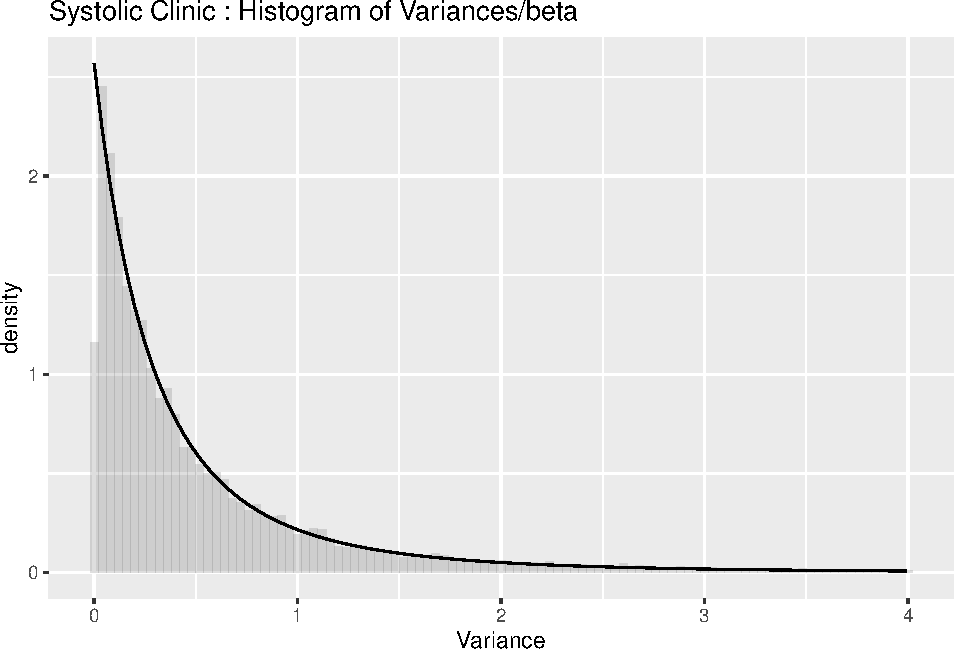
\includegraphics{NHANES-BP-Appendix_files/figure-latex/Variance test-1.pdf} 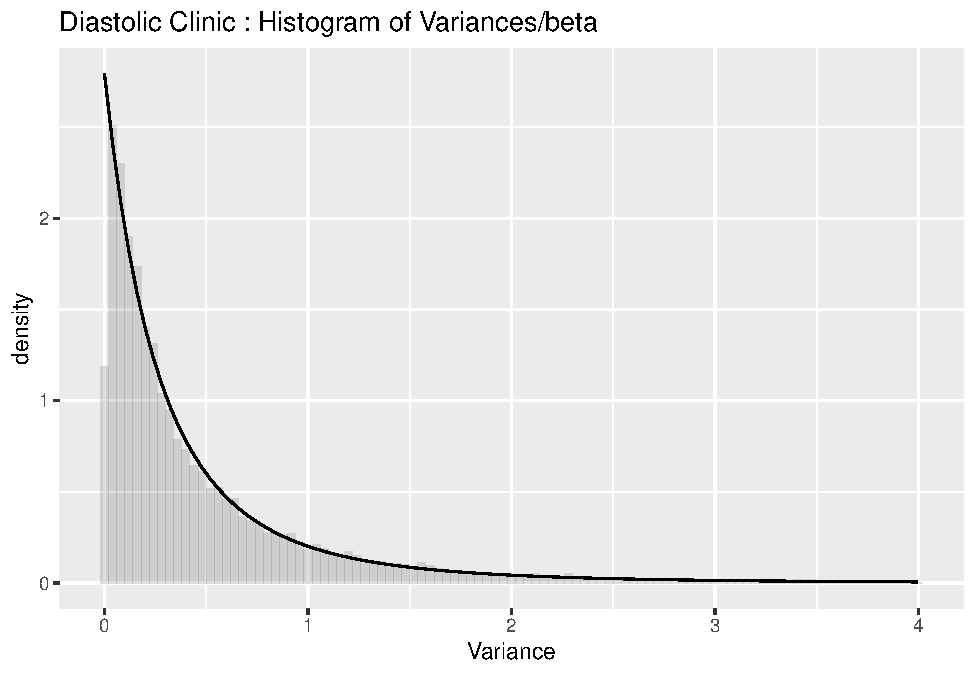
\includegraphics{NHANES-BP-Appendix_files/figure-latex/Variance test-2.pdf}
Now we generate data from the inferred model that mimic the true data, with three systolic and three diastolic BP measures per person.
These cannot be directly compared with the observed data, which are rounded to the nearest 2 (in a somewhat biased way), so we randomly impute the fractional part, which we add to the true observations.
This gives us a set of true variances and a set of simulated variances, which we hope will have approximately the same distribution.
We compare these --- for each of the four combinations of systolic/diastolic and home/clinic --- by Q--Q plots.
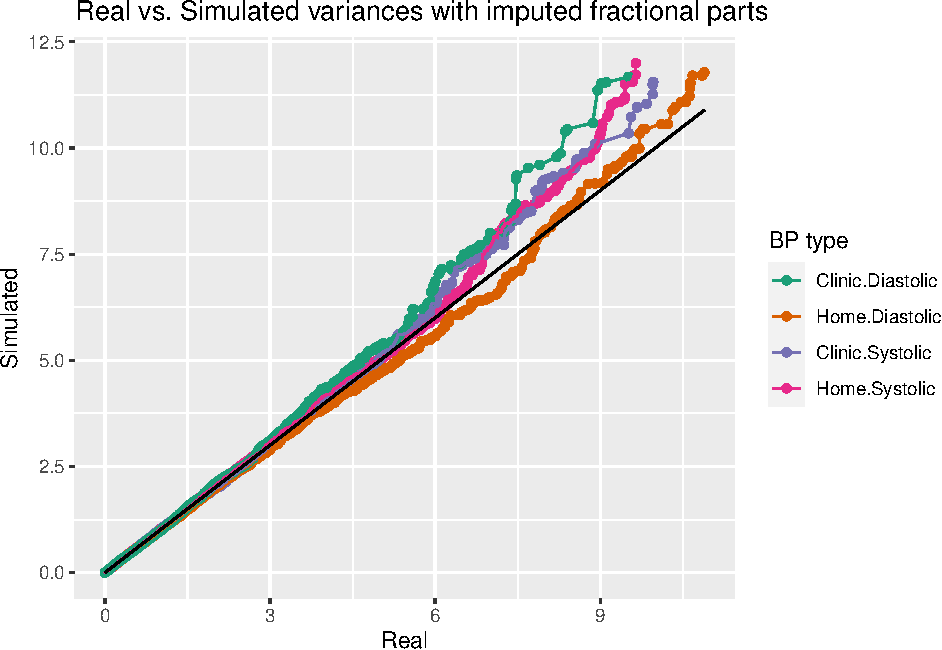
\includegraphics{NHANES-BP-Appendix_files/figure-latex/Compare_variances-1.pdf}

To finish this section, we include a table of the empirical Bayes priors, shown in tables \ref{tab:empestsS} and \ref{tab:empestsD}.

\begin{table}

\caption{\label{tab:empestsS}Empirical Bayes prior hyperparameter estimates for the systolic blood pressure for the NHANES III, full population.}
\centering
\begin{tabular}[t]{ll}
\toprule
Parameter & Estimate\\
\midrule
Clinic SD alpha & 2.5358+/-0.0057502\\
Clinic SD theta & 0.075555+/--4.9319e-05\\
Delta mu & 1.35+/-0.057989\\
Delta sigma & 6.8136+/-1.1509\\
Home SD alpha & 2.2024+/-0.0034248\\
\addlinespace
Home SD theta & 0.14809+/--7.217e-05\\
Mean mu & 123.34+/-0.16096\\
Mean sigma & 19.412+/-1.3557\\
\bottomrule
\end{tabular}
\end{table}

\begin{table}

\caption{\label{tab:empestsD}Empirical Bayes prior hyperparameter estimates for the diastolic blood pressure for the NHANES III, full population.}
\centering
\begin{tabular}[t]{ll}
\toprule
Parameter & Estimate\\
\midrule
Clinic SD alpha & 2.7914+/-0.0078652\\
Clinic SD theta & 0.10834+/--8.1306e-05\\
Delta mu & 1.0992+/-0.040354\\
Delta sigma & 4.681+/-0.94736\\
Home SD alpha & 2.299+/-0.0039401\\
\addlinespace
Home SD theta & 0.19576+/--0.00010184\\
Mean mu & 72.311+/-0.085033\\
Mean sigma & 10.198+/-1.0486\\
\bottomrule
\end{tabular}
\end{table}

\hypertarget{hamiltonian-monte-carlo-hmc}{%
\subsubsection{Hamiltonian Monte Carlo (HMC)}\label{hamiltonian-monte-carlo-hmc}}

The model, as described in the article, is a Bayesian hierarchical model. In order to parameterize such an intricate model, traditional Maximum Likelihood Estimation methods can no longer be applied. Therefore, we apply the Hamiltonian Monte Carlo (HMC) method. HMC is a form of Markov Chain Monte Carlo methods, which samples potential parameter space values of the model, then calculates directly the likelihood function based on that choice of parameters. The derivative of the likelihood function, \(\phi\), guides parameter space exploration in \(\theta\) towards the modal value of the joint posterior distribution. This method is ideal for complicated, non-Gaussian distribution forms. The three steps of HMC are:

\begin{enumerate}
\item Draw a sample of the derivative $\phi$ using the posterior distribution of $\phi$, which is the same as its prior.
\item Update the values of $\theta^*$ and $\phi^*$ using
  \begin{equation}
    \theta^*\leftarrow \theta+\epsilon M^{-1}\phi,
  \end{equation}
  and
  \begin{equation}
    \phi\leftarrow \phi+\epsilon\frac{1}{2}\frac{d\log\{p(\theta|y)\}}{d\theta},
  \end{equation}
where $M$ is the jacobian of the parameters. This can be set to a diagonal matrix for no correlation between parameters, and is pointwise updated throughout the calculation. This is the leapfrog method, whereby $\epsilon$ dictates the scale size of the step to ensure convergence on the correct point is made, and L is the number of steps to be `leaped'.
\item Compute the rejection parameter:
  \begin{equation}
    r=\frac{p(\theta^*|y)p(\phi^*)}{p(\theta^{t-1}|y)p(\phi^{t-1})}
  \end{equation}
\item Set $\theta^t$ to $\theta^*$ with probability $\min\{1,r\}$, or otherwise keep $\theta^{t-1}$.
\end{enumerate}

The tuning parameters \(\epsilon\) and L should be chosen according to a desired acceptance rate. The No-U-Turn Sampler of Stan automates the calculation of these tuning parameters. A more detailed overview of HMC and the NUTS algorithm integrated into the Stan package, see \emph{`The No-U-Turn Sampler: Adaptively Setting Path Lengths
in Hamiltonian Monte Carlo'} by M. Hoffman and A. Gelman, Journal of Machine Learning Research, 15, 1351-1381 (2014).

\hypertarget{centering-the-linear-predictor}{%
\subsubsection{Centering the Linear Predictor}\label{centering-the-linear-predictor}}

During the MCMC simulations, the centering values play a non-negligible role in shaping the model parameterization. If the centering parameters are held constant throughout all of the MCMC simulations, then the equation \(\sum_i^N \exp{(\boldsymbol{\beta}\cdot(\boldsymbol{X}-\hat{X}))}=0\) is no longer guaranteed. However, automatically defining the centering values based on the model parameters sampled at the current MCMC iteration is not advisable as it can lead to poor parameter convergence. This is because it modifies the likelihood function at every MCMC iteration. Therefore, we iterate the MCMC algorithm multiple times. At every iteration, we recalculate the centering parameters to satisfy the requirement that the average of the linear predictor term going to zero, based on the posterior distributions of the previous MCMC simulation. This iteration is carried out until the centering parameters converge. Convergence is defined by optimising on two factors. The first is that the sum of the linear predictor term across all MCMC samples needs to tend to negligible values (we define this as the average difference being less than \(10^{-7}\)), see figure \ref{fig:linpred_conv}. The second convergence criteria is that the average Root Mean-Squared Error (RMSE) of the model predictions on the survival outcomes in the MCMC simulations needs to also decrease towards zero, see figure \ref{fig:linpred_conv} (top). For the second criteria, we stopped the simulations when either the difference in the RMSE stopped decreasing (below a threshold of \(1\%\)), or the RMSE value was less than 20, see figure \ref{fig:linpred_conv} (bottom). Illustration of the convergence is shown in figure \ref{fig:linpred_conv}.

\hypertarget{code-description}{%
\subsection{Code Description}\label{code-description}}

The code can be found at \url{https://github.com/hamishwp/NHANES_HPOX}. The numerical code has been built in multiple stages. Below, we explain the principal files required to replicate the entire analysis presented in the article. There are 5 main groups for the code:

\begin{enumerate}
\def\labelenumi{\arabic{enumi}.}
\tightlist
\item
  Data cleaning scripts
\item
  Main file
\item
  Stan files for HMC
\item
  Centering recalculation scripts
\item
  Post-processing analysis
\end{enumerate}

We provide a brief description of each of these below.

\hypertarget{data-cleaning}{%
\subsubsection{Data Cleaning}\label{data-cleaning}}

This is found in the file \texttt{Dataclean2021.R}. Provided the raw NHANES dataset (in CSV format), it extracts all the data required for the simulations, and stores it in a structure that can be directly read in to the main file (\texttt{MCMC\_DiasSyst\_v3.R}) of this research.

\hypertarget{main}{%
\subsubsection{Main}\label{main}}

The main file is \texttt{MCMC\_DiasSyst\_v3.R}. It reads in the cleaned NHANES data, the specific choice of simulation parameters (for example, whether to use the FRS number or mean systolic \& diastolic blood pressure), and runs the correct RStan scripts for that specific selection of simulation parameters. This script is intended for use on computing clusters.

\hypertarget{stan}{%
\subsubsection{Stan}\label{stan}}

There are eight Stan files:

\begin{enumerate}
\def\labelenumi{\arabic{enumi}.}
\tightlist
\item
  \texttt{mystanmodel\_DS\_sigma\_v2\_autopred.stan}
\item
  \texttt{mystanmodel\_DS\_tau\_v2\_autopred.stan}
\item
  \texttt{mystanmodelFRS\_DS\_sigma\_v2\_autopred.stan}
\item
  \texttt{mystanmodelFRS\_DS\_tau\_v2\_autopred.stan}
\item
  \texttt{mystanmodel\_DS\_sigma\_v2.stan}
\item
  \texttt{mystanmodel\_DS\_tau\_v2.stan}
\item
  \texttt{mystanmodelFRS\_DS\_sigma\_v2.stan}
\item
  \texttt{mystanmodelFRS\_DS\_tau\_v2.stan}
\end{enumerate}

These correspond to the following alternative simulation parameters:

\begin{itemize}
\tightlist
\item
  For the blood-pressure variability, choosing to use the standard-deviation \(\sigma\) or the precision \(\tau=1/\sigma\){]}\}
\item
  Using the FRS score or the mean diastolic and systolic blood pressure as a covariate in the analysis
\item
  Whether the centering parameters, \(\hat{X}\), in the linear predictor term are automatically calculated to satisfy \(\sum_i^N \exp{(\boldsymbol{\beta}\cdot(\boldsymbol{X}-\hat{X}))}=0\) for every MCMC iteration, or whether the centering is held constant across all iterations
\end{itemize}

\hypertarget{centering}{%
\subsubsection{Centering}\label{centering}}

The centering of the linear predictors, which is required as input to every MCMC simulation iteration, is recalculated in the files \texttt{AutoPred\_Recalc.R} and \texttt{ManPred\_Recalc.R}. This is then provided to the Main script, \texttt{MCMC\_DiasSyst\_v3.R}, which provides these centering values to the Stan code for the MCMC simulations.

\hypertarget{empirical-bayes-estimation}{%
\subsubsection{Empirical Bayes Estimation}\label{empirical-bayes-estimation}}

The file \texttt{gamma\_fits.Rmd} contains all the necessary routines in order to replicate the calculation of the empirical Bayes' priors for the hyperparameters of the model.

\hypertarget{post-processing}{%
\subsubsection{Post-processing}\label{post-processing}}

The post-processing script is called \texttt{PostProcessing.R}, which heavily relies on the \texttt{Functions.R} script which contains all the necessary functions to analyse the data. The post-processing script generates many useful plots of the MCMC posterior distribution for the user, including Bayes' factors, violin plots of the normalised beta and gompertz posteriors, and more.

\newpage

\hypertarget{appendix-c-further-results}{%
\section{Appendix C -- Further Results}\label{appendix-c-further-results}}

In this section, we add some additional detail to the results section covered in the article. Extra information is given to explain how convergence of the simulations was ensured, and to also include more visualisations of the converged model parameterizations. The authors feel that this is particularly useful to provide confidence in the model parameterization and the predictions.

\hypertarget{convergence-of-simulations}{%
\subsubsection{Convergence of Simulations}\label{convergence-of-simulations}}

Convergence of the simulations required to parameterize the model presented in this work is required for the MCMC simulations performed by Stan, as well as convergence in the centering values that requires repeating the Stan calculations several times. Convergence of the latter is shown in figure \ref{fig:linpred_conv}. The upper plot in figure \ref{fig:linpred_conv} illustrates convergence in the average Root Mean-Squared Error (RMSE) of the model predictions on the survival outcomes in the MCMC simulations. The lower plot in figure \ref{fig:linpred_conv} illustrates convergence in the average sum of the linear predictor terms over all MCMC chain iterations.

\begin{figure}
\hypertarget{fig:linpred_conv}{%
\centering
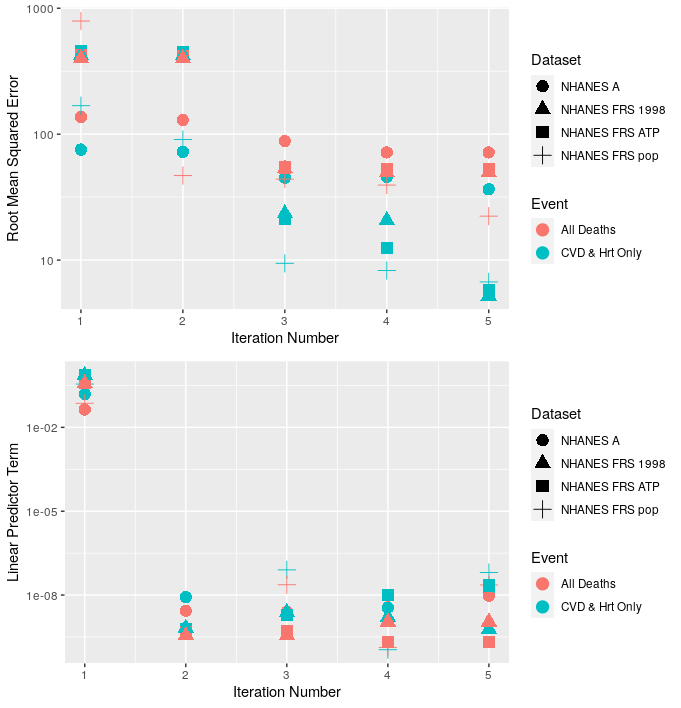
\includegraphics{./Rmarkdown_Plots/RMSE-Linpred_Convergence.png}
\caption{Illustration of the convergence of the centering parameters of the model.}\label{fig:linpred_conv}
}
\end{figure}

With respect to convergence of the MCMC simulations, defining convergence first involves discarding the burn-in period of the simulations. When the time-evolution marker chain has a large number of samples, sequence thinning is used to reduce the amount of data storage - after convergence, take only the kth value of the simulations (after having discarded the burn-in phase values) and discard the rest. One measure of convergence is to bin similar markers and check that for each bin, the variation of the individual marker movement over a few time steps is larger than the variation of the ensemble markers in-between one-another. Other methods of convergence are stationarity and mixing. The former occurs by ensuring that the gradients of movements in the chains in time are in the same direction, the latter ensures that the amplitude of the movements in the chains are similar. To calculate the mixing and stationarity, one can do the following:

\begin{itemize}
\item Take the proposedly converged marker population, where there are N markers in total each of index length $\tau$ (thus of total physical time quantity $t\tau$). Split it k times, where k is a common denominator of $\tau$.
\item Now you have $kN$ MCMC chains each of length $|\tau/k|$
\item For the marker $\psi_{ij}$ with i and j the chain length (time) and marker number indices respectively, then the mean marker value over the chain length (time) is
  \begin{equation}
    \bar{\psi}_{|,j}=\frac{k}{\tau}\sum_{i=1}^{\tau/k}\psi_{ij}
  \end{equation}
  and the total average quantity of $\psi$ over all markers, over all chain lengths is therefore
  \begin{equation}
    \bar{\psi}_{||}=\frac{1}{kN}\sum_{j=1}^{kN}\bar{\psi}_{|j}
  \end{equation}  
\item Stationarity: compare the inter-marker variance (between sequence B):
  \begin{equation}
    B = \frac{\tau}{k(kN-1)}\sum_{j=1}^{kN}(\bar{\psi}_{|,j}-\bar{\psi}_{||})^2
  \end{equation}
\item Mixing: compare the variance along each markers chain length (within-sequence W):
  \begin{equation}
    W = \frac{1}{n(\tau-k)}\sum_{j=1}^{kN}\sum_{i=1}^{\tau/k}(\psi_{i,j}-\bar{\psi}_{|j})^2
  \end{equation}
\item Therefore, to estimate the marginal posterior variance of $p(\psi|y)$, then we use a weighted average
  \begin{equation}
    \hat{\text{Var}}^+(\psi|y)=\frac{\tau-k}{N}W+\frac{1}{Nk}B
  \end{equation}
  Note that this quantity overestimates the marginal posterior variance, but it is unbiased under stationarity: this can be used to infer convergence. When the varation in
  \begin{equation}
    \hat{R}=\sqrt{\frac{\hat{\text{Var}}^+(\psi|y)}{W}}
  \end{equation}
  should approach close to 1 for converged simulations.
\end{itemize}

Another convergence parameter is the number of effective independent marker draws. Upon convergence, the time evolution of each marker should be uncorrelated and independent to previous time steps. To find the average time-correlation over all particles, we use the variogram \(V_t\):
\begin{equation}
  V_t=\frac{1}{Nk(\tau/k-\tilde{t})}\sum_{j=1}^{kN}\sum_{i=1}^{\tau/k}(\psi_{i,j}-\psi_{i-\tilde{t},j})^2,
\end{equation}
where \(\tilde{t}\in 1,2,...,\tau/k\) is a time index. Then we get the time-correlations:
\begin{equation}
  \hat{\rho}_t=1-\frac{V_t}{2\hat{\text{Var}}^+}
\end{equation}
This comes from the expectation of the variance \(E[(\psi_i-\psi_{i-t})^2]=2(1-\rho_t)\text{Var}(\psi)\). This can be used to infer the effective number of independent marker draws:
\begin{equation}
  \hat{n}_{eff}=\frac{mn}{1+2\sum_{\tilde{t}=1}^T\hat{\rho}_t}
\end{equation}
Where T is the index at which the sum of the autocorrelation estimates \(\hat{\rho}_{t'}+\hat{\rho}_{t'+1}\) is negative. As a general guide, we should have \(\hat{n}_{eff}\sim 10N/k\) effective independent marker draws and that \(\hat{R}\to 1\sim 1.1\). In this research, we continued running the MCMC simulations until these two criteria were met (and went beyond: \(\hat{R}<1.05\) for all parameters in all models and that \(\hat{n}_{eff}>750\) for all parameters in all models).

\hypertarget{results---model-parameterization}{%
\subsubsection{Results - Model Parameterization}\label{results---model-parameterization}}

We remind the reader of the list of numbers of the different models explored in this research, provided in the list found in section `Proposed Models'. The authors will use the numbers in the list, referred to as the run number, in the following plots. One of the most important set of parameters of the model is the vector \(\beta\) of covariates in the Cox' proportional hazards model. When the \(\beta\) vector is normalised, the larger (in absolute terms) the value of \(\beta\), the larger the correlation between that specific covariate and the risk of mortality. Positive values of \(\beta\) imply a higher risk of mortality, and the inverse for negative values of \(\beta\). As we can see from the violin plots of the MCMC posterior samples of the \(\beta\) parameters in figure \ref{fig:betas}, the parameter that correlated the highest with both the mortality risk of HA-CVD-CeVD and for all mortalities, in absolute terms, was the 1998 version of the FRS score, shown in the top-right plot under run numbers 7 and 8. The FRS-1998 score correlated, on average over all the MCMC iterations, approximately \(25\%\) more with mortality risk of HA-CVD-CeVD than the (more recently developed) FRS ATP III score. A similar, but slightly weaker, correlation was found between the two FRS scores for all mortality-based risk. The middle-left plot in figure \ref{fig:betas} shows that the mean diastolic blood pressure acts to decrease mortality risk. Finally, the influence of the longer-term difference in the mean blood pressure, displayed in the top-left and top-middle plots of figure \ref{fig:betas}, is also shown to increase mortality risk across all run numbers. The influence of the blood-pressure variability on mortality is illustrated to not be consistent across simulations, whereby the statistical significance of the effect is lower than for the other parameters in the linear predictor term.

\begin{figure}
\hypertarget{fig:betas}{%
\centering
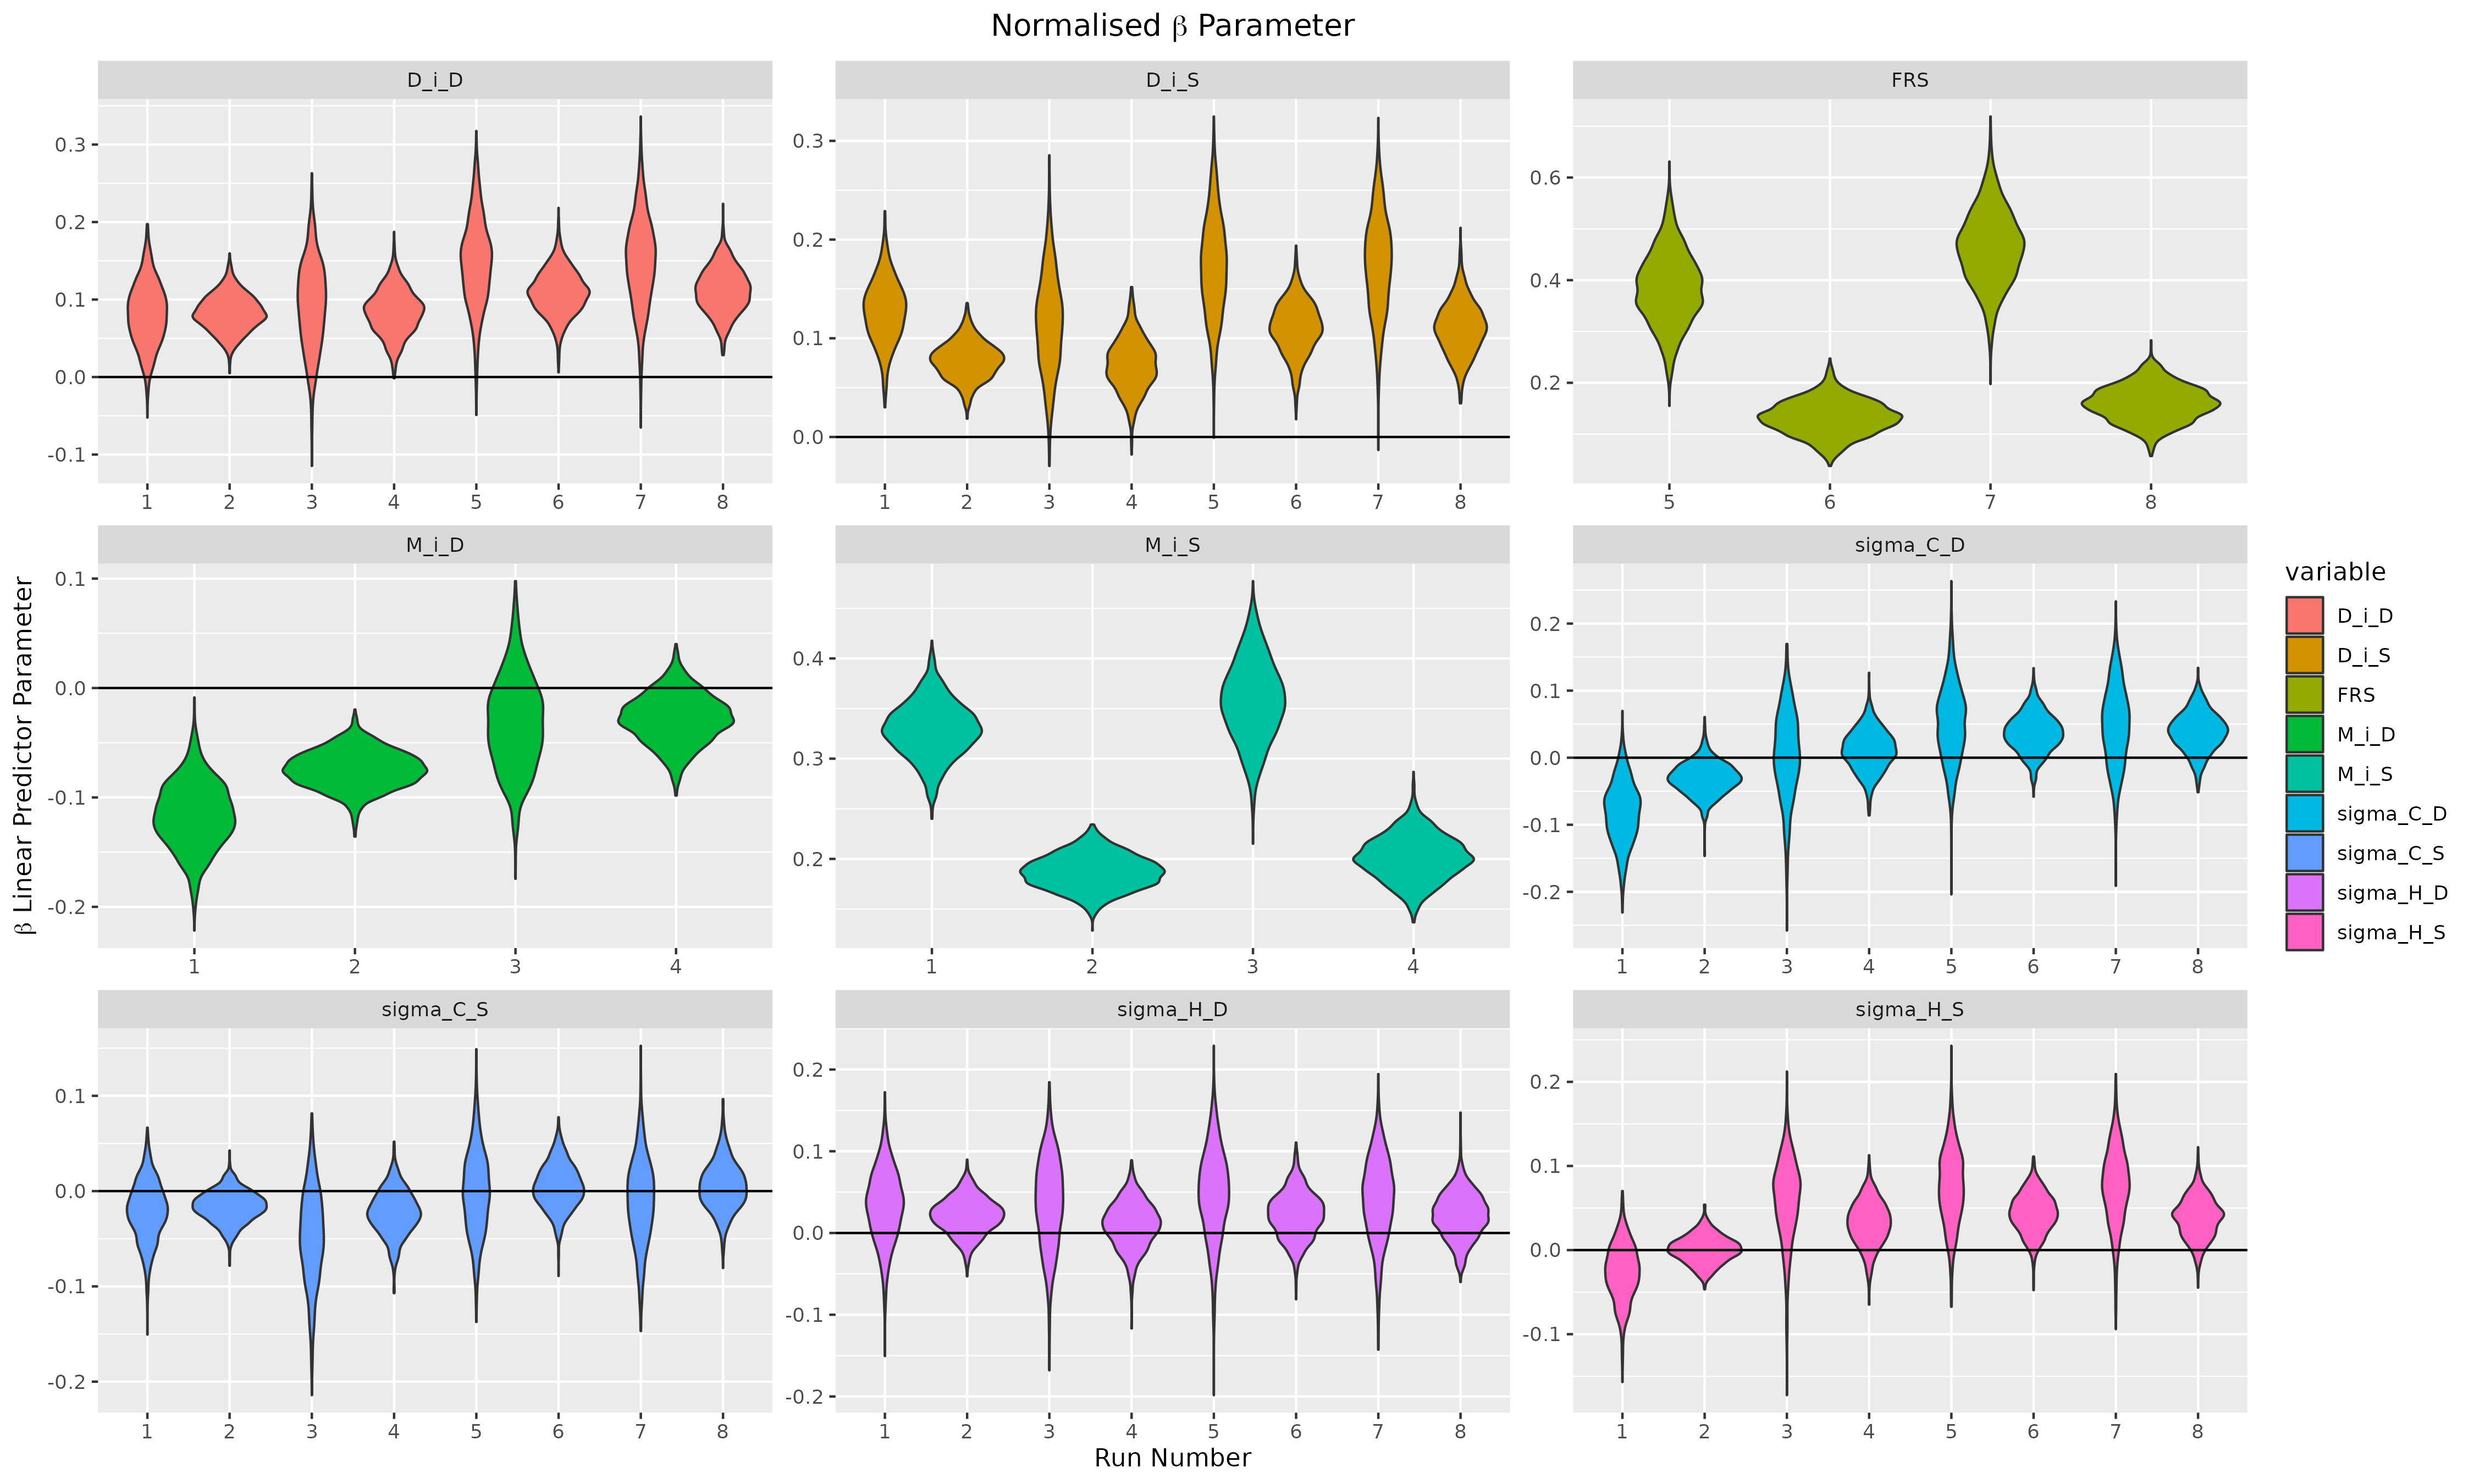
\includegraphics{./Plots/beta/Beta_parameter_normalised.png}
\caption{Violin plots of the normalised \(\beta\) parameters of the different models.}\label{fig:betas}
}
\end{figure}

With respect to the time-independent Gompertz parameter, described using \(B\) in this article, the results between all models that simulate HA-CVD-CeVD mortality risk, and all the models that simulation all-cause mortality risk are consistent with one-another. This is illustrated by the similarity between plots on the left hand side and the right hand side of figure \ref{fig:gompB}. The consistency appears across sex assigned at birth and race.

\begin{figure}
\hypertarget{fig:gompB}{%
\centering
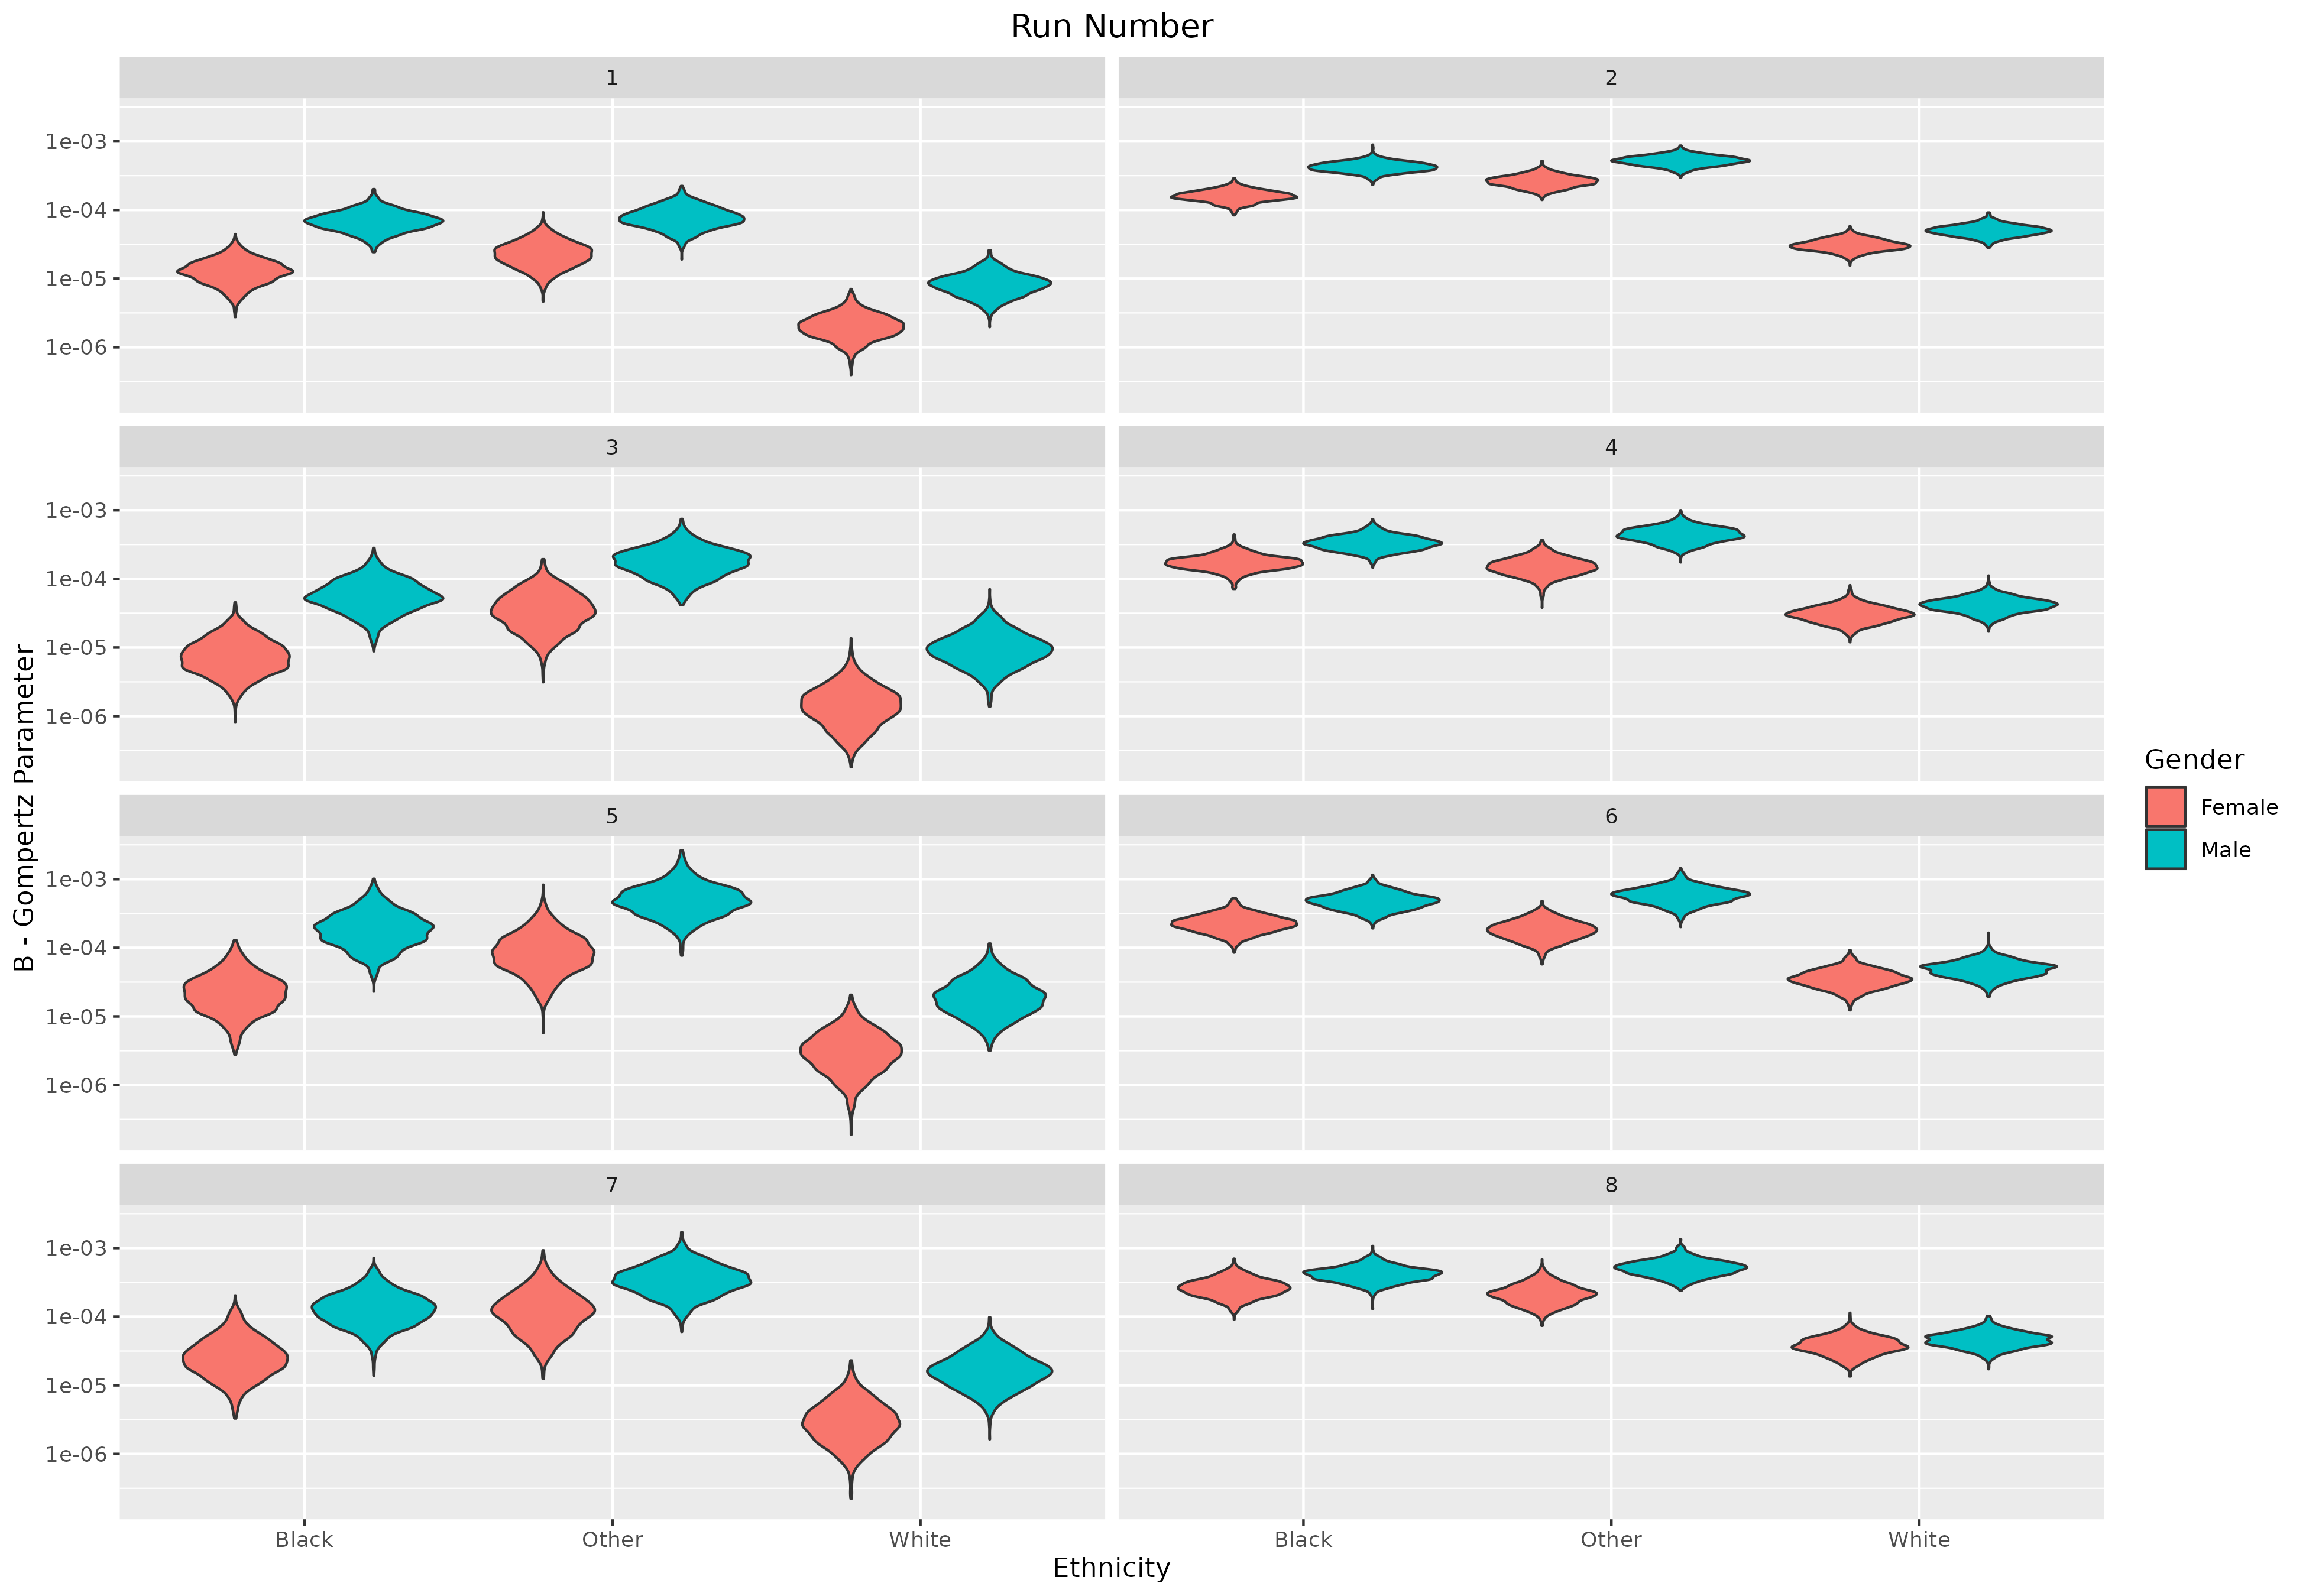
\includegraphics{./Plots/gompertz/B_parameter.png}
\caption{Violin plots of the normalised B parameter (from the Gompertz equation) of the different models.}\label{fig:gompB}
}
\end{figure}

Figure \ref{fig:gompt} reflects the same level of consistency for the Gompertz parameter that influences the temporal evolution of the mortality risk. It is worth noting that both figures \ref{fig:gompB} and \ref{fig:gompt} have inverse trends between the values of B and theta for each demographic group. This makes it difficult to imagine, based on these two plots, what the mortality risk is at different ages across demographics, yet it is evident that the form of the change in the mortality risk curve in time is different for each demographic group. Women are observed to have lower initial values of risk, but mortality risk later in life begins to increase much faster than for men. Additionally, hispanic populations are shown to have a larger initial mortality risk than black populations who are shown to have a larger initial mortality risk than white populations in the USA. However, mortality risk increases at a faster rate for white populations than for black populations, for which it increases faster than hispanic populations in the USA. For ease of comparison, we also present here tables of the mean and standard deviation values of the time dependent and independent Gompertz parameters in tables \ref{tab:RL12} to \ref{tab:RL78}.

\begin{figure}
\hypertarget{fig:gompt}{%
\centering
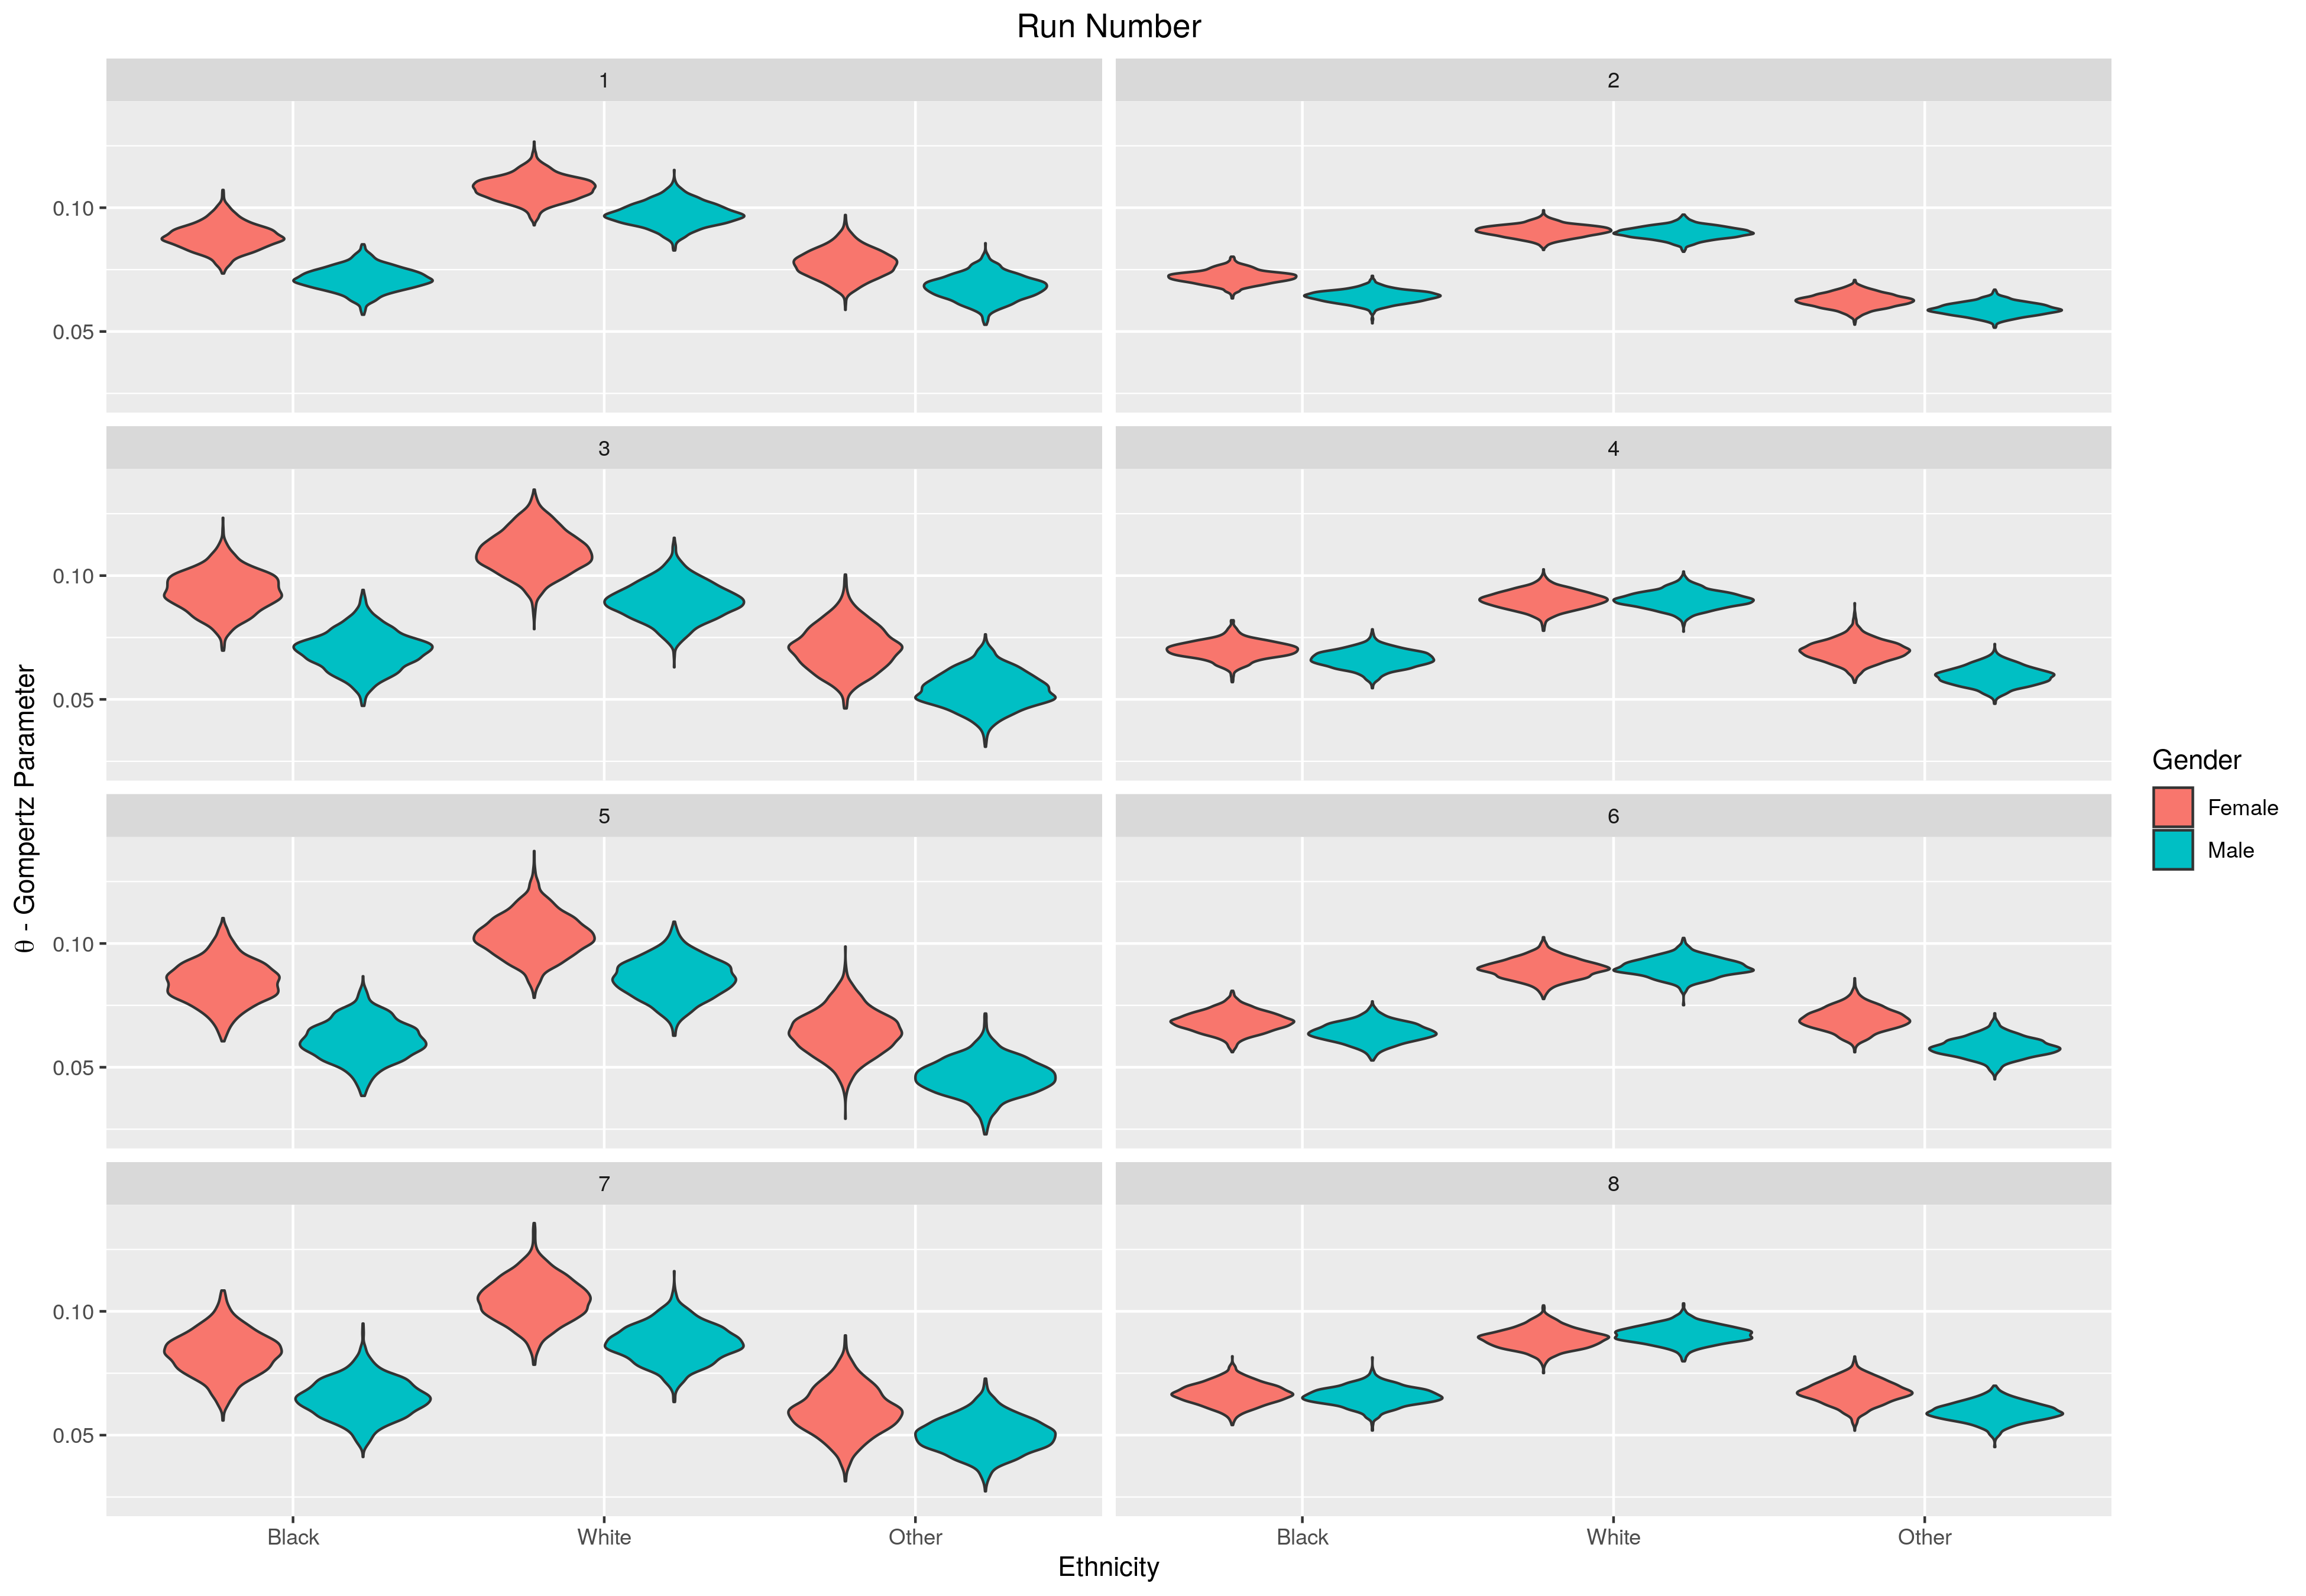
\includegraphics{./Plots/gompertz/theta_parameter.png}
\caption{Violin plots of the normalised \(\theta\) parameter (from the Gompertz equation) of the different models.}\label{fig:gompt}
}
\end{figure}

\begin{table}

\caption{\label{tab:RL12}Parameters for survival model for HA-CVD-CeVD and all-cause mortality, NHANES III, Full population, using the systolic and diastolic mean model.}
\centering
\begin{tabular}[t]{llrrrr}
\toprule
Sex & Race/Ethnicity & B–Mean & B–SD & $\theta$-Mean & $\theta$–SD\\
\midrule
Female & Black & 1.36e-05 & 5.70e-06 & 0.0883 & 0.00534\\
Female & White & 2.20e-06 & 9.00e-07 & 0.1080 & 0.00488\\
Female & Other & 2.44e-05 & 1.07e-05 & 0.0775 & 0.00565\\
Male & Black & 7.20e-05 & 2.49e-05 & 0.0712 & 0.00459\\
Male & White & 8.70e-06 & 3.40e-06 & 0.0973 & 0.00466\\
\addlinespace
Male & Other & 8.17e-05 & 3.00e-05 & 0.0678 & 0.00498\\
\bottomrule
\end{tabular}
\end{table}

\begin{table}

\caption{\label{tab:RL34}Parameters for survival model for HA-CVD-CeVD and all-cause mortality, NHANES III, FRS-population only, using the systolic and diastolic mean model.}
\centering
\begin{tabular}[t]{llrrrr}
\toprule
Sex & Race/Ethnicity & B–Mean & B–SD & $\theta$-Mean & $\theta$–SD\\
\midrule
Female & Black & 8.60e-06 & 5.40e-06 & 0.0937 & 0.00795\\
Female & White & 1.70e-06 & 1.30e-06 & 0.1100 & 0.00844\\
Female & Other & 4.06e-05 & 2.65e-05 & 0.0708 & 0.00879\\
Male & Black & 6.36e-05 & 3.53e-05 & 0.0697 & 0.00765\\
Male & White & 1.08e-05 & 6.50e-06 & 0.0896 & 0.00737\\
\addlinespace
Male & Other & 1.94e-04 & 9.69e-05 & 0.0539 & 0.00709\\
\bottomrule
\end{tabular}
\end{table}

\begin{table}

\caption{\label{tab:RL78}Parameters for survival model for HA-CVD-CeVD and all-cause mortality, NHANES III, FRS-population only, using the 1998 FRS-based model.}
\centering
\begin{tabular}[t]{llrrrr}
\toprule
Sex & Race/Ethnicity & B–Mean & B–SD & $\theta$-Mean & $\theta$–SD\\
\midrule
Female & Black & 2.62e-05 & 1.82e-05 & 0.0843 & 0.00859\\
Female & White & 3.70e-06 & 2.70e-06 & 0.1030 & 0.00861\\
Female & Other & 1.02e-04 & 7.46e-05 & 0.0641 & 0.00896\\
Male & Black & 2.14e-04 & 1.34e-04 & 0.0608 & 0.00793\\
Male & White & 2.22e-05 & 1.46e-05 & 0.0859 & 0.00778\\
\addlinespace
Male & Other & 5.58e-04 & 3.25e-04 & 0.0461 & 0.00720\\
\bottomrule
\end{tabular}
\end{table}

\hypertarget{results---model-performance}{%
\subsubsection{Results - Model Performance}\label{results---model-performance}}

To measure the performance of the model to predict the survival outcome of individuals in the population, figure \ref{fig:cumpred} shows, ordered by individual age, the cumulative hazard \(H(t)\) predicted against the cumulative number of deaths in the populations, for each model explored in this research. Each model is shown to predict survival outcomes reliably, across the entire age range of the population.

\begin{figure}
\hypertarget{fig:cumpred}{%
\centering
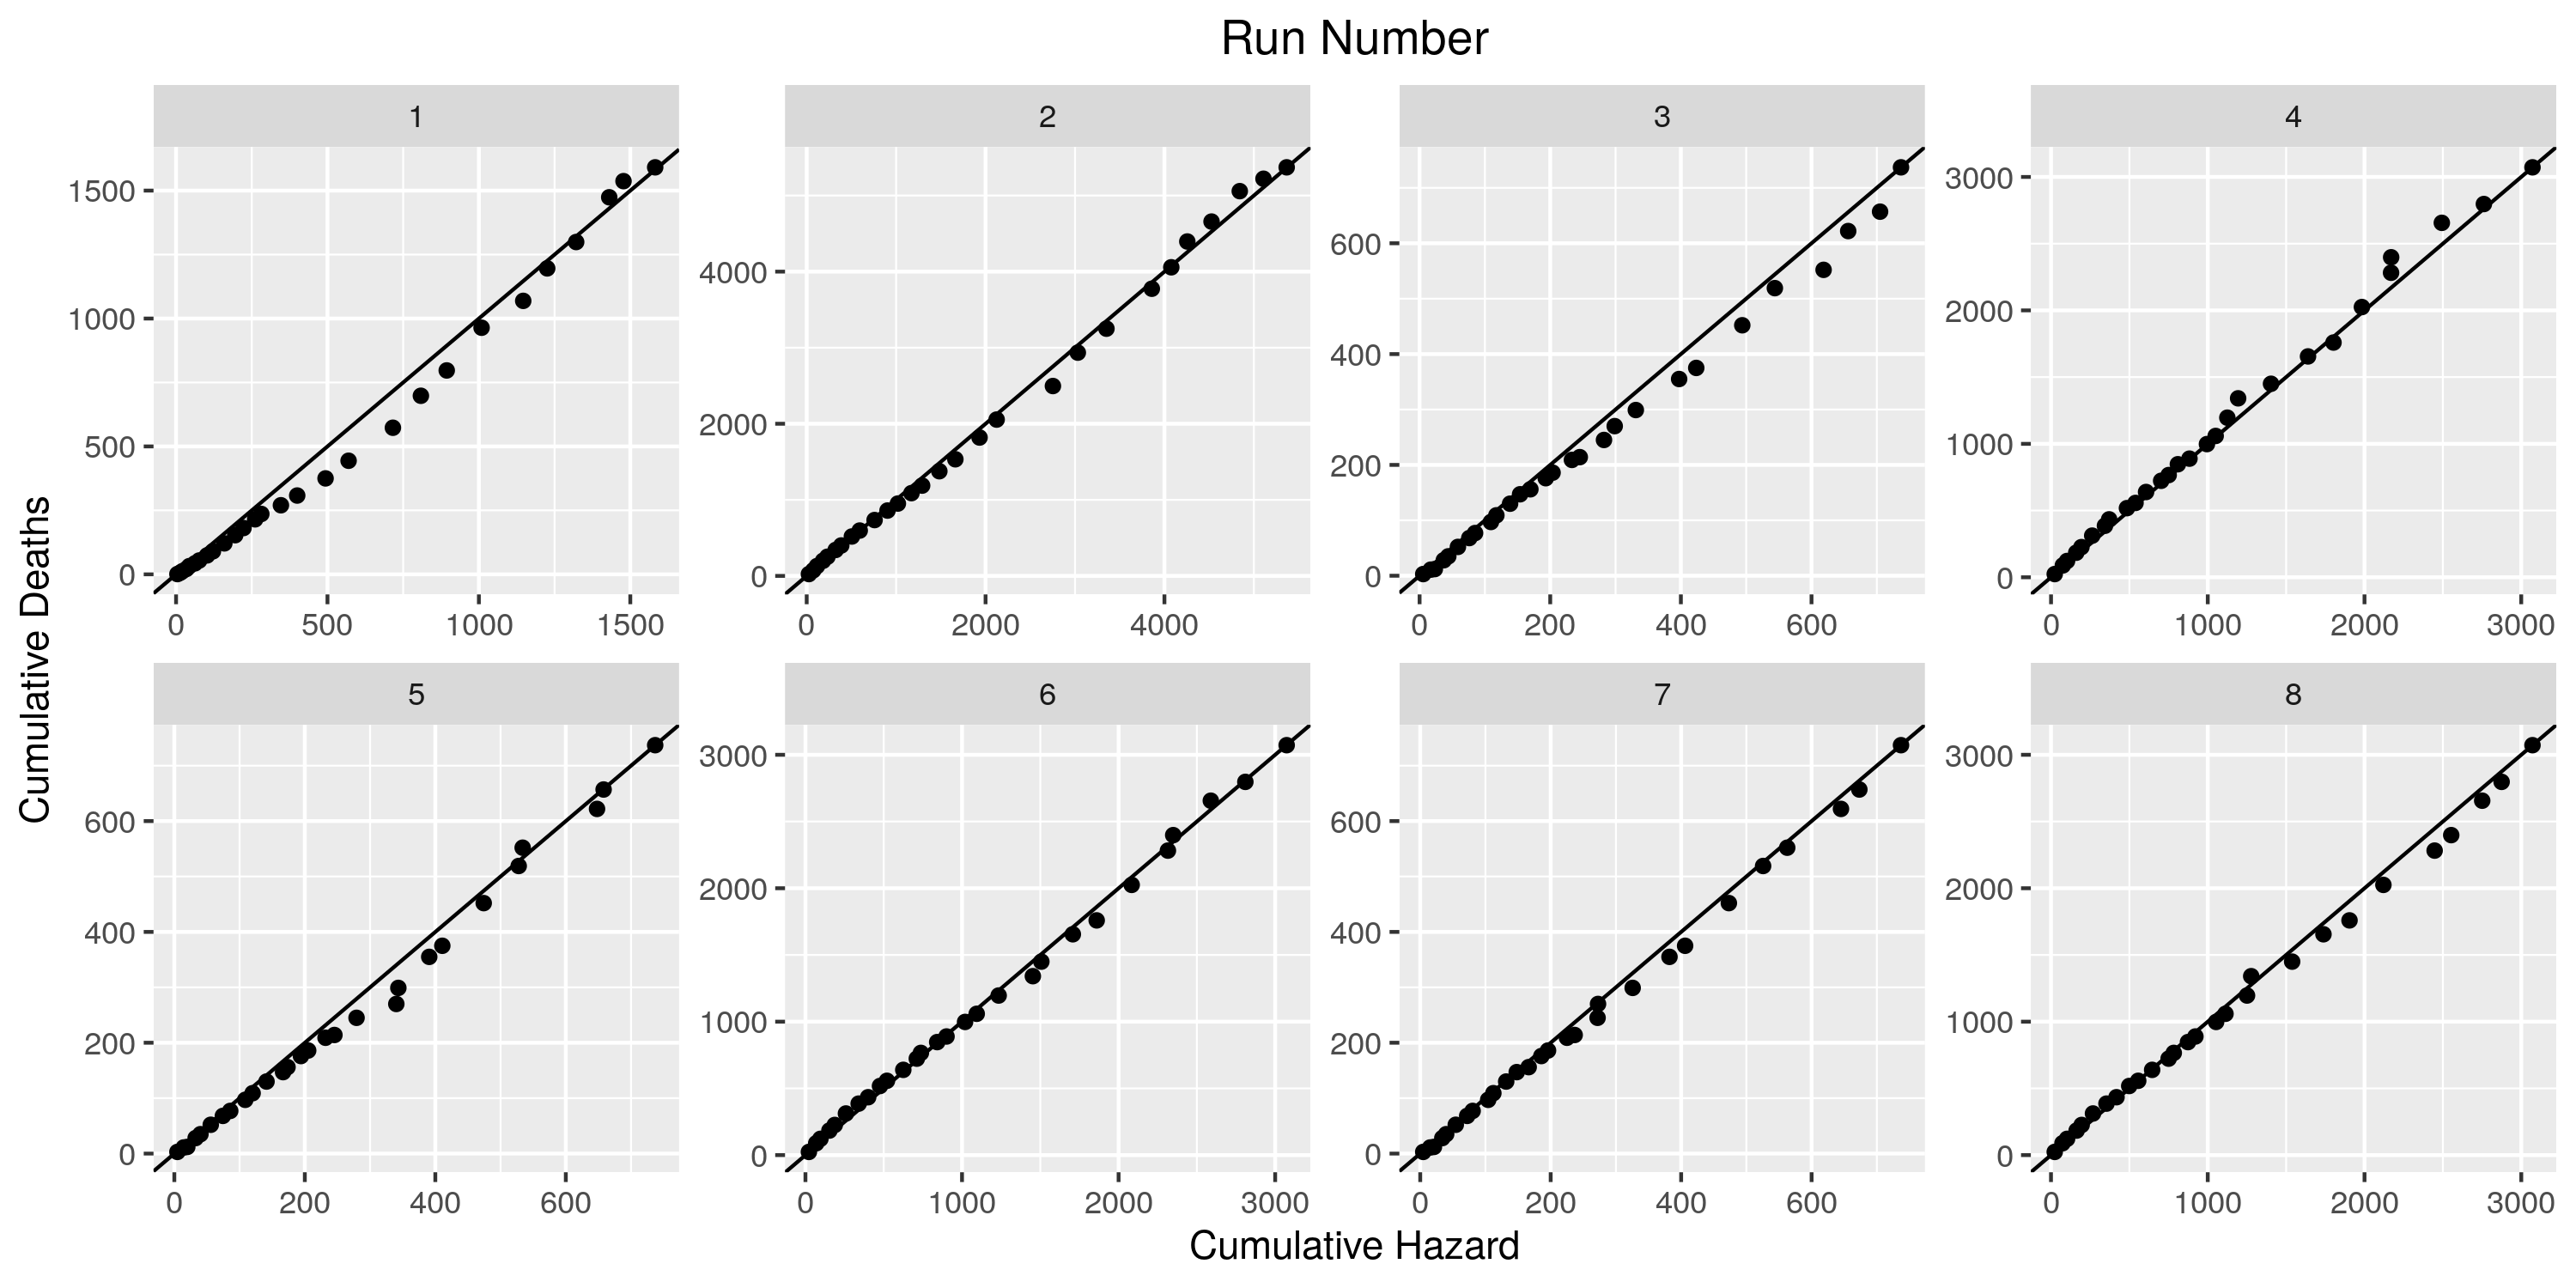
\includegraphics{./Plots/Survival/redlinpred_Cumulative_haz-death_age.png}
\caption{Predicted cumulative hazard against cumulative number of deaths in the population, ordered by the age of the individual.}\label{fig:cumpred}
}
\end{figure}

A common metric that is used to evaluate the performance of models such as presented in this article is called the Receiver Operating Characteristic (ROC) curve. With continuous predictor values such as cumulative hazard \(H(T_i)\), a threshold can be defined whereby any individual who has a cumulative risk larger than the threshold \(H(T_i)>\epsilon\) is predicted to die. The ratio of the number individuals that were predicted to die compared to the total number who die corresponds is referred to as the True Positive Ratio (TPR)
\begin{equation}
  TPR(\epsilon)=\frac{\sum_i\big(\mathbb{I}(H(T_i)>\epsilon \ \ \& \ \ \delta_i=1)\big)}{\sum_i\big(\mathbb{I}(\delta_i=1)\big)}.
\end{equation}
Note that TPR is also referred to as the recall or sensitivity. Conversely, the ratio of the number of individuals predicted to die but survive compared to the total number of individuals that survived is referred to as the False Positive Ratio (FPR)
\begin{equation}
  FPR(\epsilon)=\frac{\sum_i\big(\mathbb{I}(H(T_i)>\epsilon \ \ \& \ \ \delta_i=0)\big)}{\sum_i\big(\mathbb{I}(\delta_i=0)\big)}.
\end{equation}
Note that the FPR is also referred to as \(1-\mathrm{specificity}\). The ROC curve is produced by varying the threshold value that is then used to calculate both the TPR and FPR, and plotting them against one another. The area under this curve is a metric that indicates performance of the model to predict survival outcomes. AUROC=1 implies perfect predictions and AUROC=0.5 implies the contrary. However, our model is formulated such that the variables age and time since starting the survey both form part of Cox's proportional hazard. Furthermore, the Gompertz model is stratified by demographic group. Therefore, in this work, we present a modified ROC curve, which calculates the individuals cumulative hazard at a given time since the start of the survey, \(T_{surv} \in {5, 10, 15}\) years, and calculates whether the model correctly predicted an event to occur before or after this time. Note that to do this, we split the ROC population by ages: 45-64 and 65-84. The modified TPR is then calculated via:
\begin{equation}
  TPR(\epsilon)=\frac{\sum_i\big(\mathbb{I}(\delta_i=1 \ \ \& \ \ \ H(T_i)\geq \epsilon \ \ \& \ \ T_i<T_{surv})\big)}{\sum_i\big(\mathbb{I}(\delta_i=1 \ \ \& \ \ \ T_i<T_{surv})\big)},
\end{equation}
and the modified FPR:
\begin{equation}
  FPR(\epsilon)=\frac{\sum_i\big(\mathbb{I}(H(T_i)\geq \epsilon \ \ \& \ \ T_i\geq T_{surv})\big)}{\sum_i\big(\mathbb{I}(T_i\geq T_{surv})\big)}.
\end{equation}
Before presenting any ROC or AUC values, we first present the density distributions of the median posterior systolic \(\Delta\) values for all individuals, split by demographic.

\begin{figure}
\hypertarget{fig:DeltaDens}{%
\centering
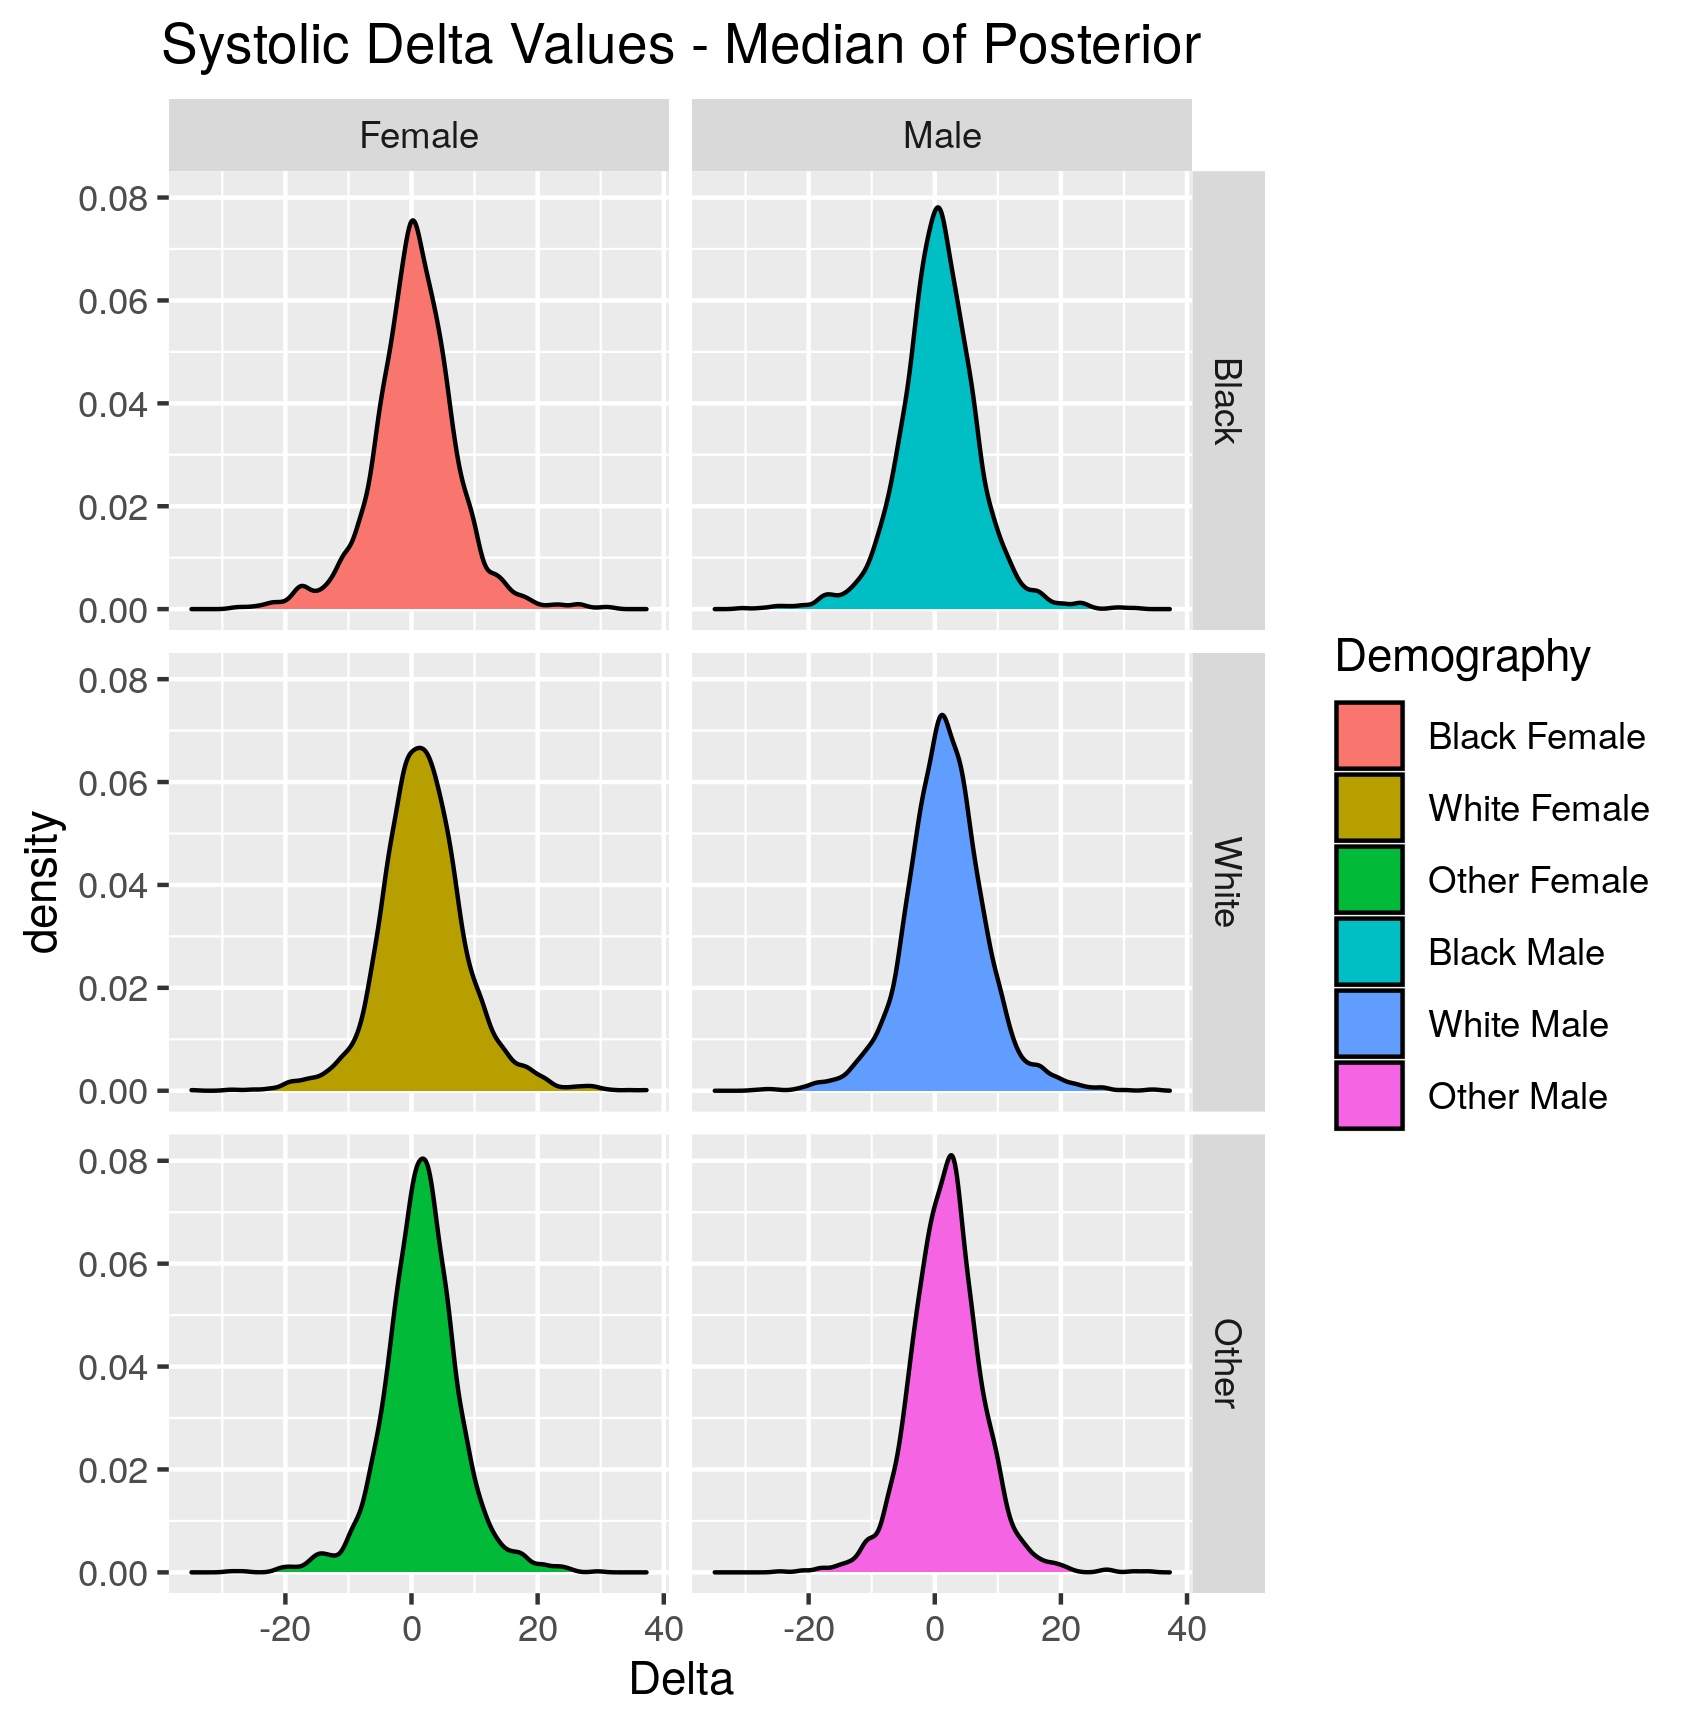
\includegraphics{./Rmarkdown_Plots/SysDelta_Densities_Demography.png}
\caption{Density of the (median posterior) systolic \(\Delta\) values, per demographic.}\label{fig:DeltaDens}
}
\end{figure}

Using Welch's ANOVA test, we calculated that \(p<1\times 10^{-9}\) for all demographics, including when split between the male and female populations. Figures \ref{fig:ROC_MeanBP} and \ref{fig:ROC_FRS} show the ROC curves (including the AUC values) of the model, the former using the mean systolic and diastolic blood pressure as covariates in the linear predictor term (in the Cox's proportional hazards component) and the latter using the FRS value instead. By making predictions of the 5, 10 and 15 year survival between the middle aged and old aged sub-groups, for the three different mortality causes, we start to build a picture of the performance of the model. For figure \ref{fig:ROC_MeanBP}, we notice that the AUC value of the predictions for the middle aged compared to the older aged population is higher, independent of the survival year prediction or the different mortality causes. The highest AUC is for the 45-64 year old population with a focus on HA-CVD-CeVD and heart attack-related mortality, for all three survival year periods. We also note that the TPR seems to start increasing at a faster rate for the population aged 45-64 than the 65-84 group, implying that it is possible to choose a threshold level, \(\epsilon\), for the survival predictions that could correctly identify people at risk without incorrectly predicting as many people to be at risk of mortality as for the group aged 65-84. The results also reflect that the influence of choosing a 5, 10 or 15 year prediction period does not seem to significantly influence the results. Figure \ref{fig:ROC_FRS} displays similar results to the mean systolic and diastolic model when using the FRS value instead, with the main difference that the predictions of the middle aged group for HA-CVD-CeVD and heart attack-related mortality for 5 year survival seems to be lower than the equivalent in the older group or as compared to the mean blood pressure model. This is caused by a reduced mortality before 5 years for the middle aged population that had their FRS value calculated, where 36, 83 and 213 HA-CVD-CeVD and heart attack-related deaths occurred before 5, 10 and 15 years in this sub-group, respectively. This can be compared to 141, 356 and 952 all-cause deaths in this same sub-group (red-curve in figure \ref{fig:ROC_FRS} and \ref{fig:ROC_MeanBP}). Alternatively, when compared to the full-population (not just those who had the FRS value), the HA-CVD-CeVD and heart attack-related deaths for the middle aged population are 55, 115 and 282 over the 5, 10 and 15 year range, respectively.

\begin{figure}
\hypertarget{fig:ROC_MeanBP}{%
\centering
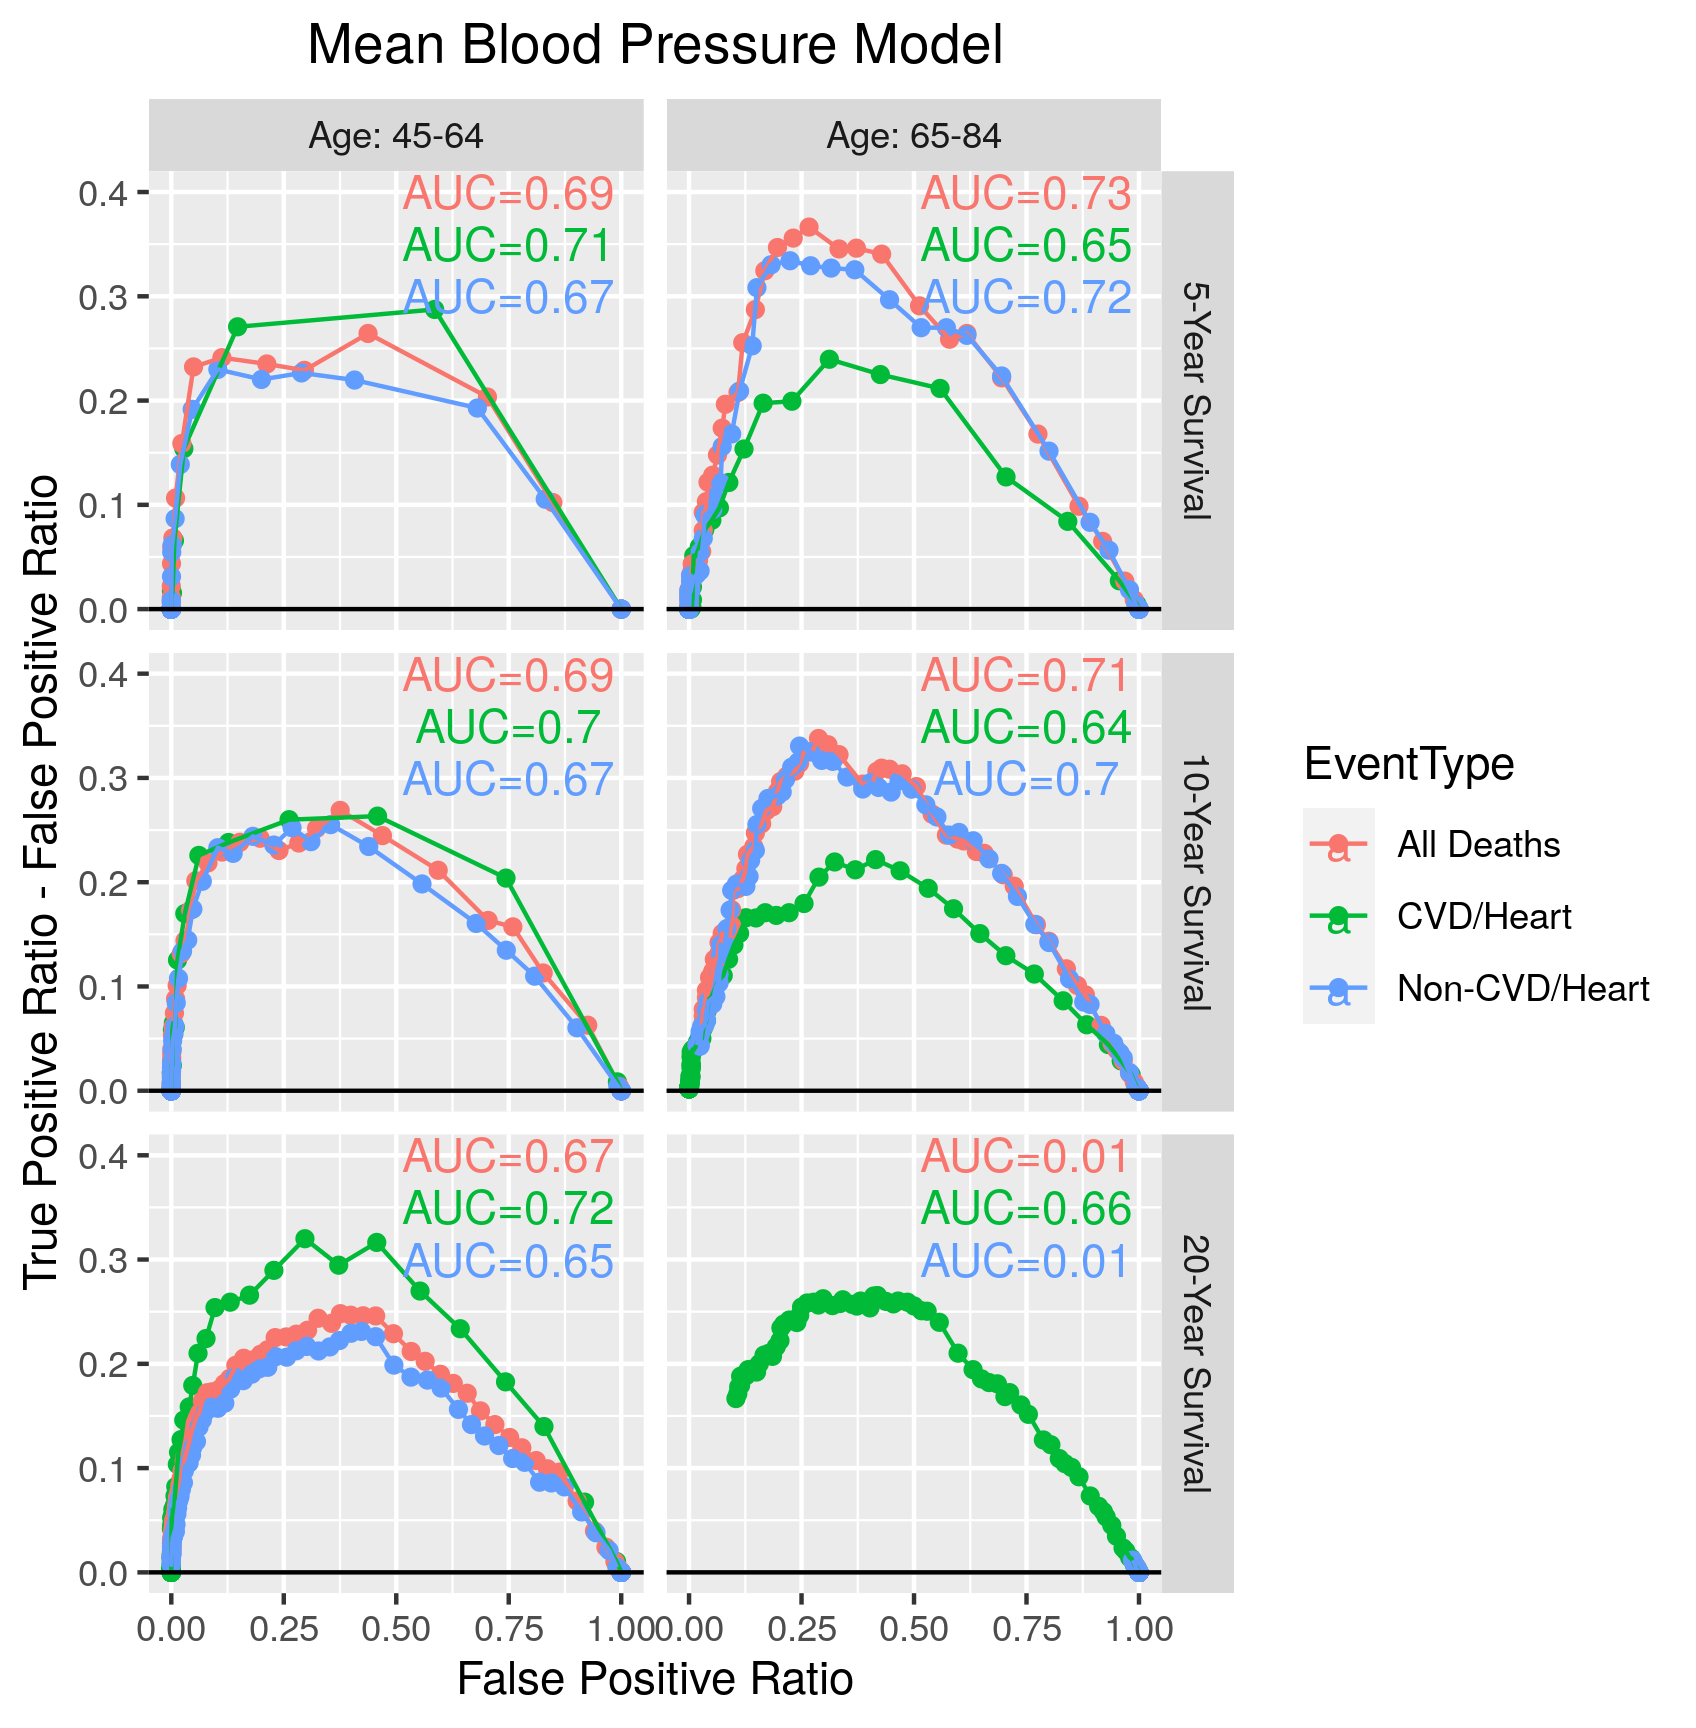
\includegraphics{./Rmarkdown_Plots/ROC_MeanBPModel_CAx-EventType.png}
\caption{ROC curves for the model that used mean systolic and diastolic blood pressure as covariates in the linear predictor, stratified by the event type (cause of mortality). The columns split two groups in the population: those who start the survey aged between 45 to 64 and 65-84 years old. The rows split the model predictions between 5, 10 and 2 year survival.}\label{fig:ROC_MeanBP}
}
\end{figure}

\begin{figure}
\hypertarget{fig:ROC_FRS}{%
\centering
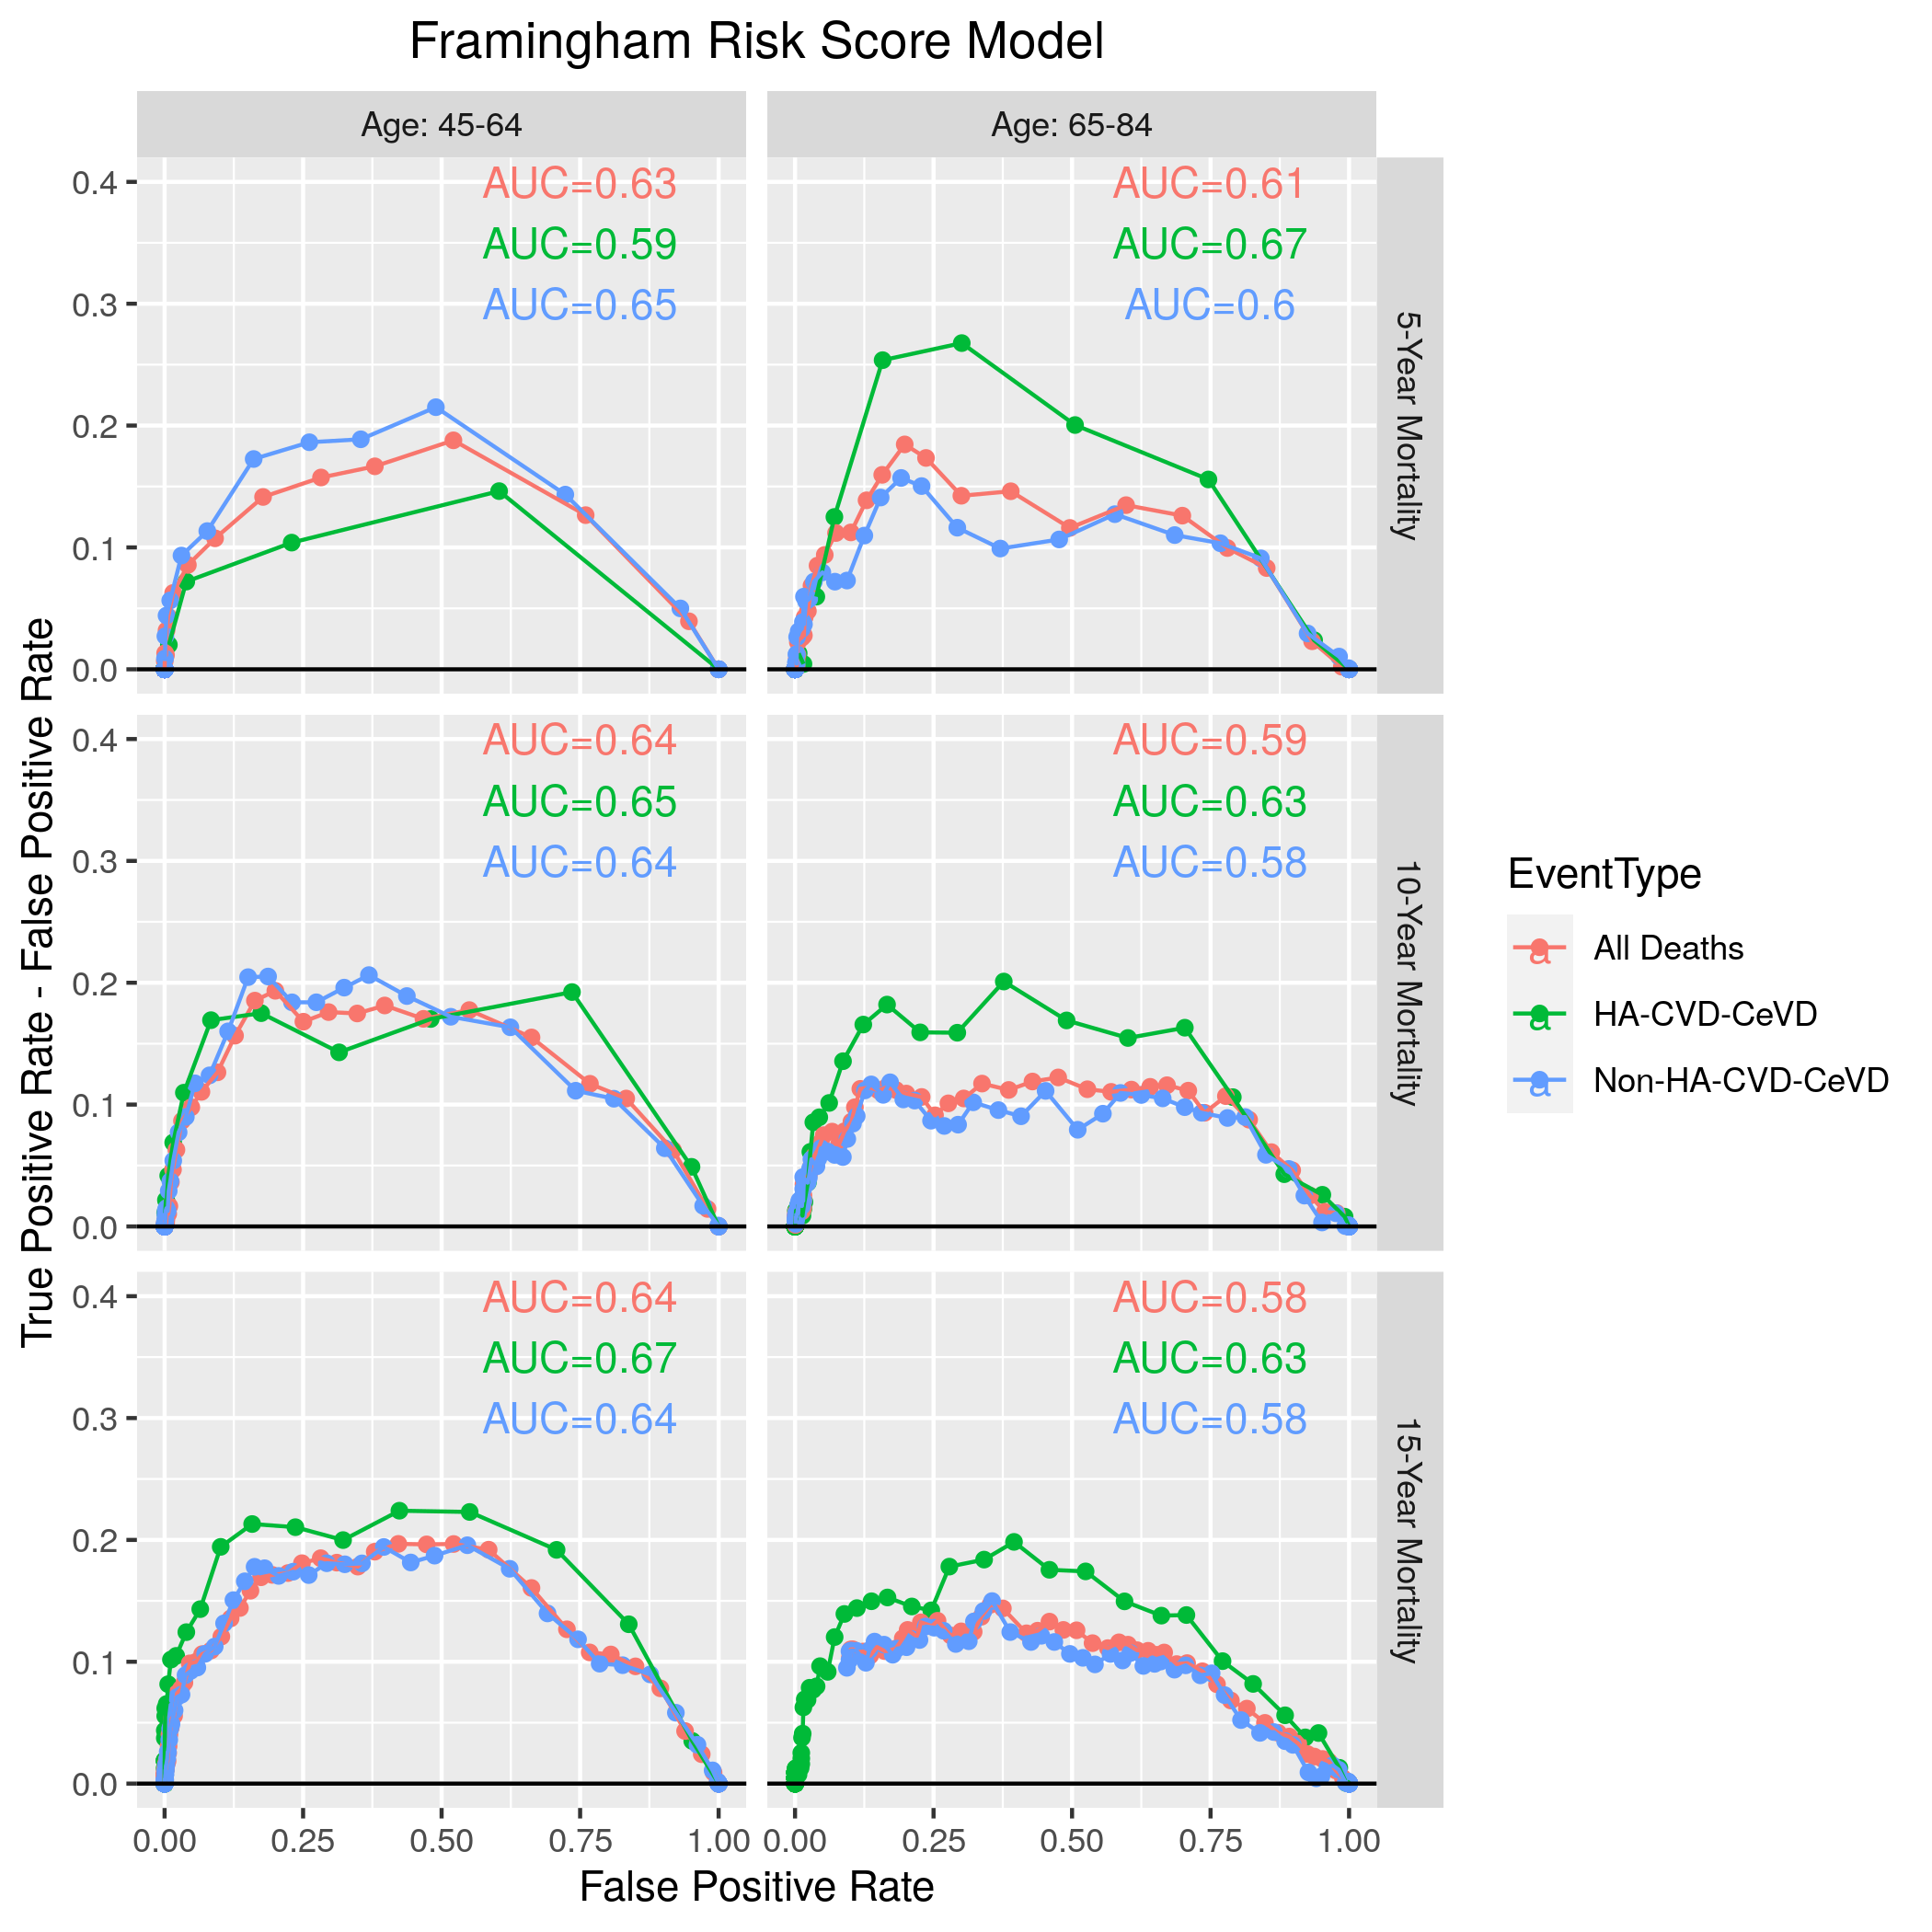
\includegraphics{./Rmarkdown_Plots/ROC_FRSModel_CAx-EventType.png}
\caption{ROC curves for the model that used the FRS value as covariates in the linear predictor, stratified by age group and the number of years the survival outcome was predicted since participant starting the survey.}\label{fig:ROC_FRS}
}
\end{figure}

Comparison of the ROC curves and AUC values is also presented for the different demographic groups, see figure \ref{fig:ROC_Demog}. This figure shows the differences in the prediction performance (w.r.t. the ROC and AUC values) of the full-population model for the 45-64 age population for their 10 year survival outcome, using the mean systolic and diastolic blood pressure model. This plot illustrates that potentially only the all-cause mortality has enough outcomes in each demographic group to separate the ROC curves. The model seems to most accurately predict the 10 year survival outcome of the black and other ethnic groups, as well as the white female demographic as compared to the black female, other female and white male population. To provide insight into this, we also provide the frequency table of deaths for each demographic group, mortality cause and survival year, see table \ref{tab:DeathFreq1} and \ref{tab:DeathFreq2}.

\begin{figure}
\hypertarget{fig:ROC_Demog}{%
\centering
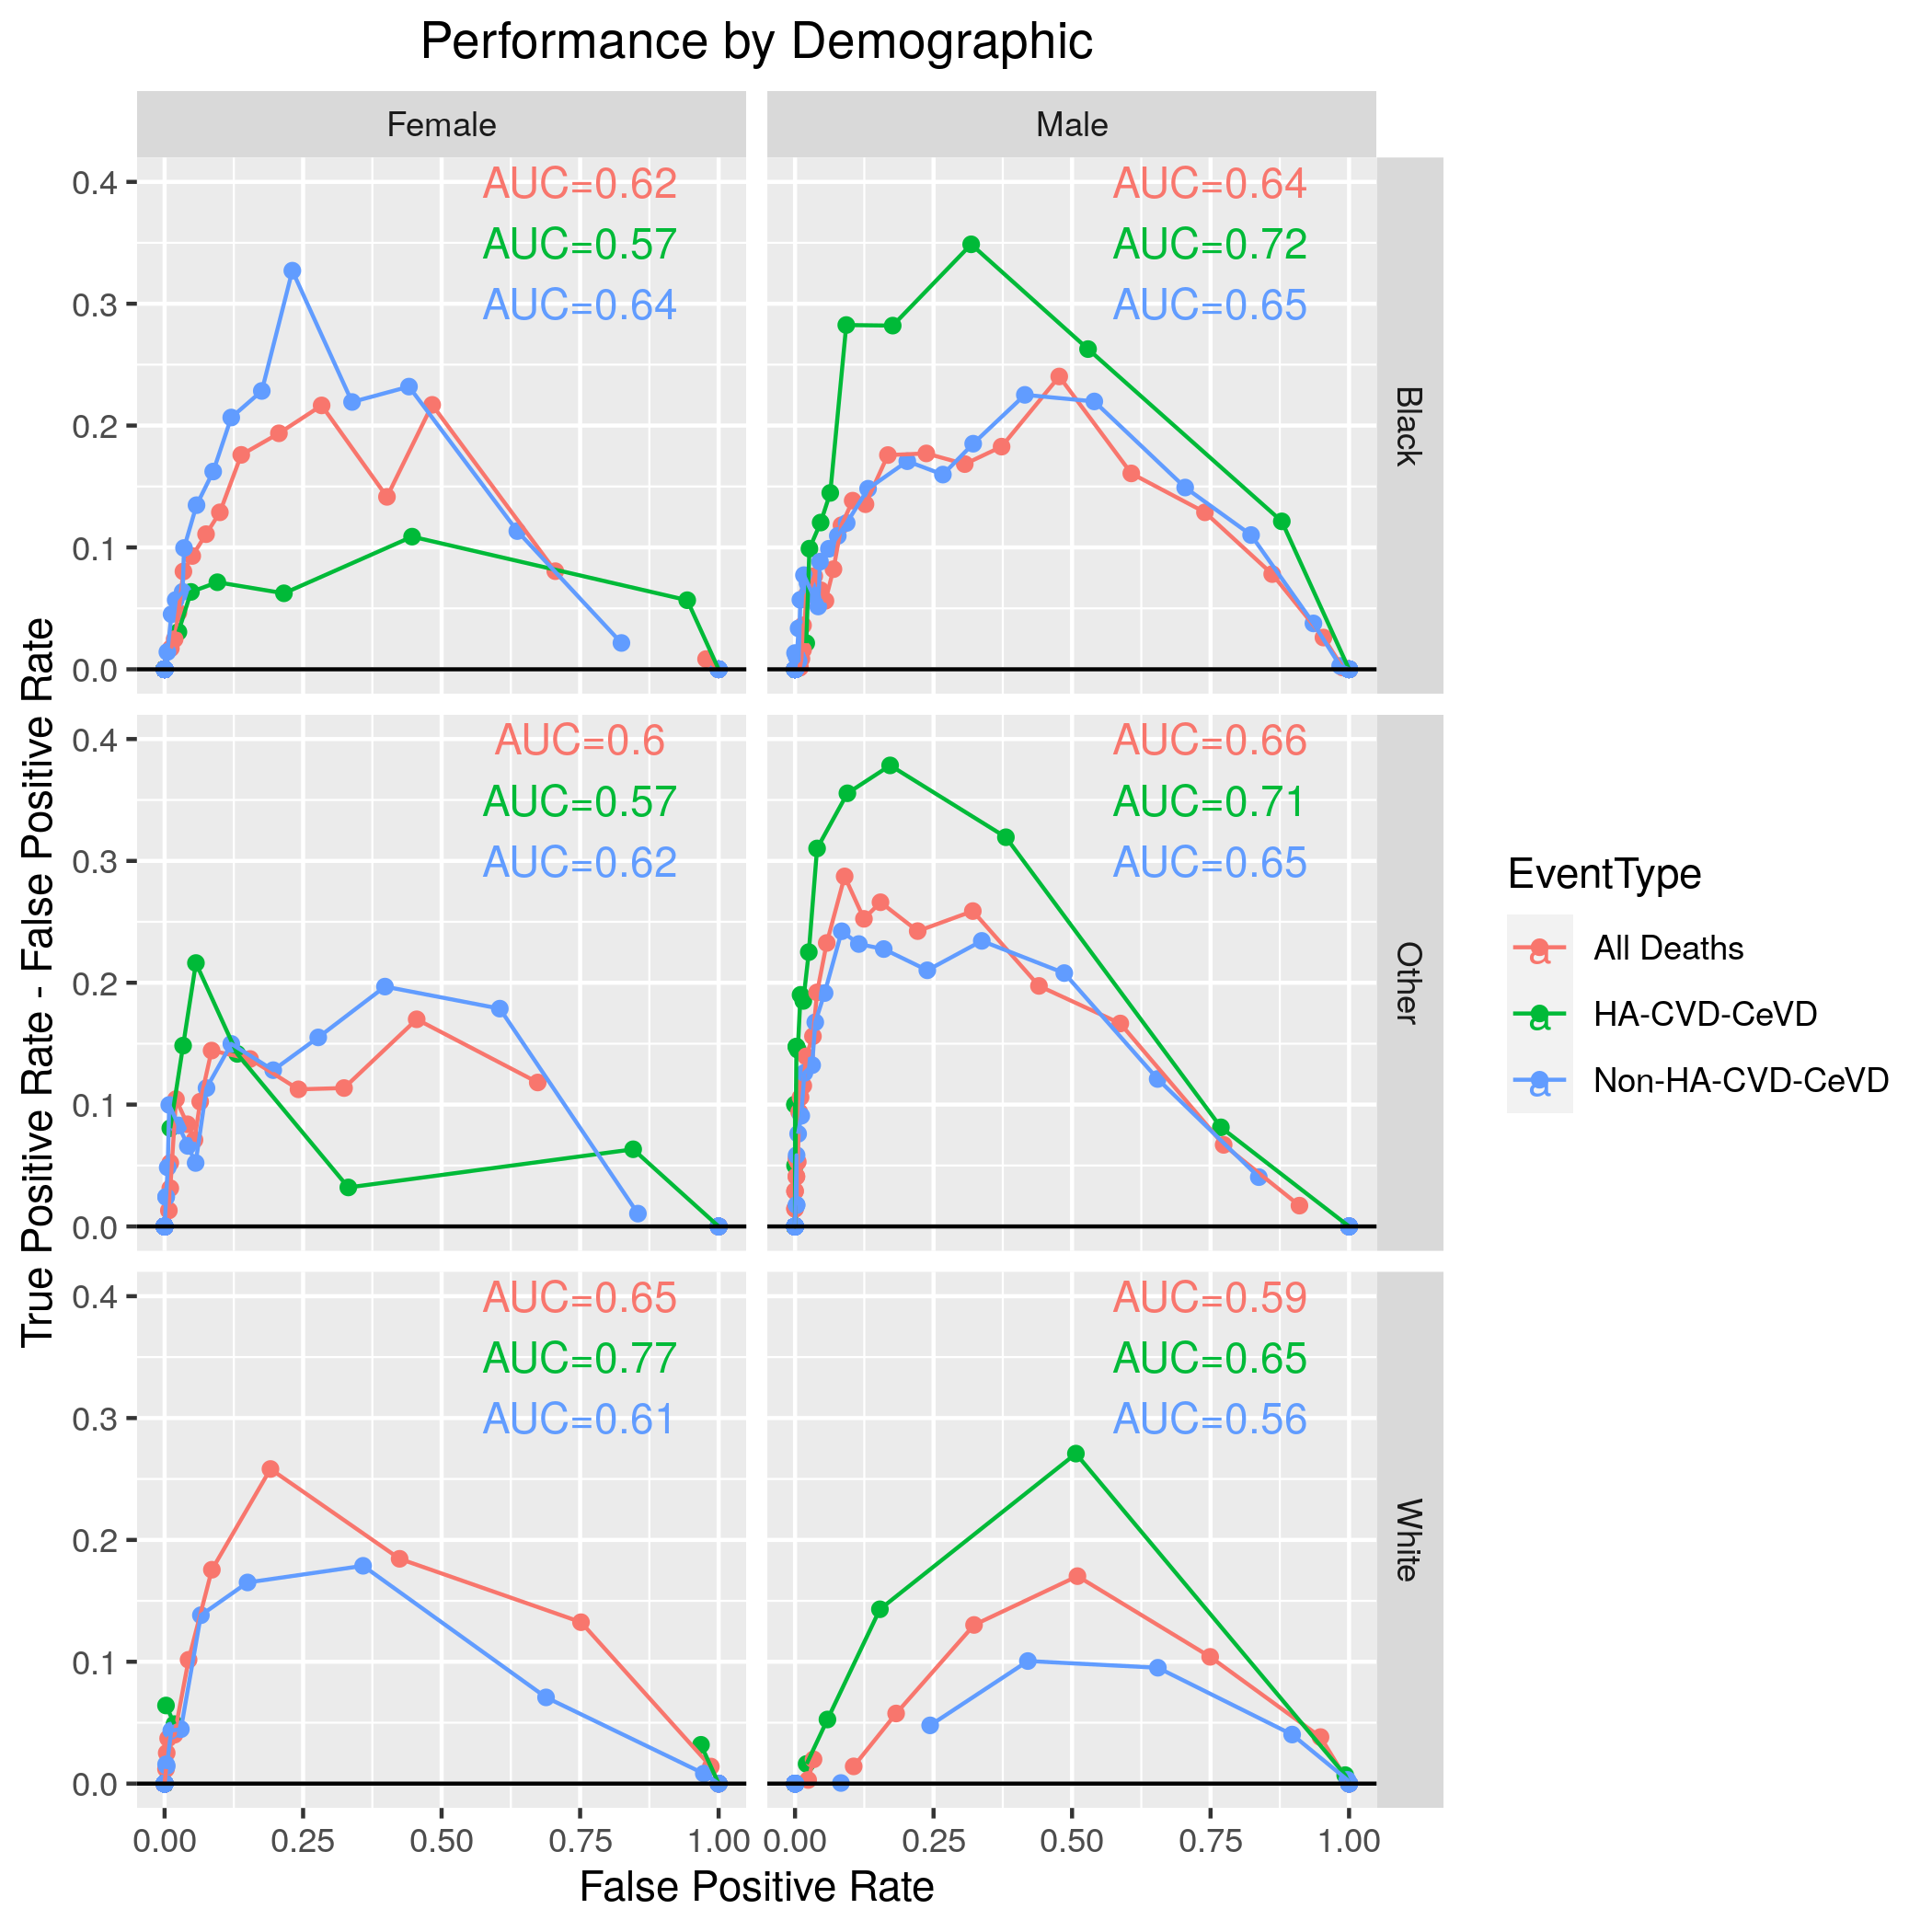
\includegraphics{./Rmarkdown_Plots/ROC_CAx-EventType_Demog_10Yr_45-64.png}
\caption{ROC curves stratified by the different demographic groups used in this research. The point and line colours represent the different event types that were used to predict on.}\label{fig:ROC_Demog}
}
\end{figure}

\begin{table}

\caption{\label{tab:DeathFreq1}Frequency table of the population aged 45-64 for the N-year survival outcomes as separated by demographic group and mortality cause.}
\centering
\begin{tabular}[t]{llllr}
\toprule
Year & EventType & Ethnicity & Gender & Deaths\\
\midrule
5-Year Mortality & HA-CVD-CeVD & Black & Female & 15\\
5-Year Mortality & All Deaths & Black & Female & 44\\
5-Year Mortality & HA-CVD-CeVD & White & Female & 9\\
5-Year Mortality & All Deaths & White & Female & 33\\
5-Year Mortality & HA-CVD-CeVD & Other & Female & 9\\
\addlinespace
5-Year Mortality & All Deaths & Other & Female & 24\\
5-Year Mortality & HA-CVD-CeVD & Black & Male & 6\\
5-Year Mortality & All Deaths & Black & Male & 25\\
5-Year Mortality & HA-CVD-CeVD & White & Male & 7\\
5-Year Mortality & All Deaths & White & Male & 24\\
\addlinespace
5-Year Mortality & HA-CVD-CeVD & Other & Male & 6\\
5-Year Mortality & All Deaths & Other & Male & 21\\
10-Year Mortality & HA-CVD-CeVD & Black & Female & 23\\
10-Year Mortality & All Deaths & Black & Female & 87\\
10-Year Mortality & HA-CVD-CeVD & White & Female & 21\\
\addlinespace
10-Year Mortality & All Deaths & White & Female & 67\\
10-Year Mortality & HA-CVD-CeVD & Other & Female & 19\\
10-Year Mortality & All Deaths & Other & Female & 63\\
10-Year Mortality & HA-CVD-CeVD & Black & Male & 17\\
10-Year Mortality & All Deaths & Black & Male & 67\\
\addlinespace
10-Year Mortality & HA-CVD-CeVD & White & Male & 13\\
10-Year Mortality & All Deaths & White & Male & 62\\
10-Year Mortality & HA-CVD-CeVD & Other & Male & 10\\
10-Year Mortality & All Deaths & Other & Male & 44\\
15-Year Mortality & HA-CVD-CeVD & Black & Female & 37\\
\addlinespace
15-Year Mortality & All Deaths & Black & Female & 132\\
15-Year Mortality & HA-CVD-CeVD & White & Female & 44\\
15-Year Mortality & All Deaths & White & Female & 139\\
15-Year Mortality & HA-CVD-CeVD & Other & Female & 35\\
15-Year Mortality & All Deaths & Other & Female & 105\\
\addlinespace
15-Year Mortality & HA-CVD-CeVD & Black & Male & 26\\
15-Year Mortality & All Deaths & Black & Male & 113\\
15-Year Mortality & HA-CVD-CeVD & White & Male & 29\\
15-Year Mortality & All Deaths & White & Male & 117\\
15-Year Mortality & HA-CVD-CeVD & Other & Male & 18\\
\addlinespace
15-Year Mortality & All Deaths & Other & Male & 67\\
\bottomrule
\end{tabular}
\end{table}

\begin{table}

\caption{\label{tab:DeathFreq2}Frequency table of the population aged 65-84 for the N-year survival outcomes as separated by demographic group and mortality cause.}
\centering
\begin{tabular}[t]{llllr}
\toprule
Year & EventType & Ethnicity & Gender & Deaths\\
\midrule
5-Year Mortality & HA-CVD-CeVD & Black & Female & 35\\
5-Year Mortality & All Deaths & Black & Female & 87\\
5-Year Mortality & HA-CVD-CeVD & White & Female & 92\\
5-Year Mortality & All Deaths & White & Female & 253\\
5-Year Mortality & HA-CVD-CeVD & Other & Female & 15\\
\addlinespace
5-Year Mortality & All Deaths & Other & Female & 45\\
5-Year Mortality & HA-CVD-CeVD & Black & Male & 19\\
5-Year Mortality & All Deaths & Black & Male & 49\\
5-Year Mortality & HA-CVD-CeVD & White & Male & 55\\
5-Year Mortality & All Deaths & White & Male & 138\\
\addlinespace
5-Year Mortality & HA-CVD-CeVD & Other & Male & 10\\
5-Year Mortality & All Deaths & Other & Male & 29\\
10-Year Mortality & HA-CVD-CeVD & Black & Female & 56\\
10-Year Mortality & All Deaths & Black & Female & 153\\
10-Year Mortality & HA-CVD-CeVD & White & Female & 187\\
\addlinespace
10-Year Mortality & All Deaths & White & Female & 501\\
10-Year Mortality & HA-CVD-CeVD & Other & Female & 37\\
10-Year Mortality & All Deaths & Other & Female & 105\\
10-Year Mortality & HA-CVD-CeVD & Black & Male & 50\\
10-Year Mortality & All Deaths & Black & Male & 121\\
\addlinespace
10-Year Mortality & HA-CVD-CeVD & White & Male & 144\\
10-Year Mortality & All Deaths & White & Male & 357\\
10-Year Mortality & HA-CVD-CeVD & Other & Male & 44\\
10-Year Mortality & All Deaths & Other & Male & 91\\
15-Year Mortality & HA-CVD-CeVD & Black & Female & 79\\
\addlinespace
15-Year Mortality & All Deaths & Black & Female & 231\\
15-Year Mortality & HA-CVD-CeVD & White & Female & 251\\
15-Year Mortality & All Deaths & White & Female & 694\\
15-Year Mortality & HA-CVD-CeVD & Other & Female & 56\\
15-Year Mortality & All Deaths & Other & Female & 170\\
\addlinespace
15-Year Mortality & HA-CVD-CeVD & Black & Male & 76\\
15-Year Mortality & All Deaths & Black & Male & 185\\
15-Year Mortality & HA-CVD-CeVD & White & Male & 225\\
15-Year Mortality & All Deaths & White & Male & 589\\
15-Year Mortality & HA-CVD-CeVD & Other & Male & 57\\
\addlinespace
15-Year Mortality & All Deaths & Other & Male & 139\\
\bottomrule
\end{tabular}
\end{table}

To finalise the section on the performance of the models using ROC and AUC values, we present a series of figures that provide ROC curves and AUC values for different linear predictor (Cox's proportional hazards model) covariate configurations. By setting the covariate-specific \(\beta\) parameter values to zero, we can measure the additional prediction performance that adding different covariates provides to the model. In figures \ref{fig:ROC_RL1} to \ref{fig:ROC_RL8oth}, we present three main formulations: using only the systolic and diastolic \(\Delta\) terms, using the mean systolic and diastolic (figures \ref{fig:ROC_RL1}-\ref{fig:ROC_RL2oth}) or the FRS value (figures \ref{fig:ROC_RL7}-\ref{fig:ROC_RL8oth}) terms as well as the systolic and diastolic \(\Delta\) terms (figures \ref{fig:ROC_RL1}-\ref{fig:ROC_RL8oth}) and, finally, using the systolic mean (figures \ref{fig:ROC_RL1}-\ref{fig:ROC_RL2oth}) or FRS value only (figures \ref{fig:ROC_RL7}-\ref{fig:ROC_RL8oth}). Figures \ref{fig:ROC_RL1}, \ref{fig:ROC_RL2} and \ref{fig:ROC_RL2oth} apply to the full-population with the models trained on HA-CVD-CeVD and heart-attack related mortality, all-cause, and other mortality, respectively. Figures \ref{fig:ROC_RL7}, \ref{fig:ROC_RL8} and \ref{fig:ROC_RL8oth} apply to the population with an FRS value, with the models trained on HA-CVD-CeVD and heart-attack related mortality, all-cause, and other mortality, respectively. The first thing to note as a commonality between all these different figures is that the use of the long-term variability, \(\Delta\), in the model has comparable performance with that of using the systolic mean or FRS values only. Additionally, where the number of deaths permits for prediction, the use of both the \(\Delta\) and mean/FRS values results in higher AUC values than using models that use one or the other. Finally, the use of the FRS value consistently under-performs the mean diastolic and systolic blood pressure-based model.

\begin{figure}
\hypertarget{fig:ROC_RL1}{%
\centering
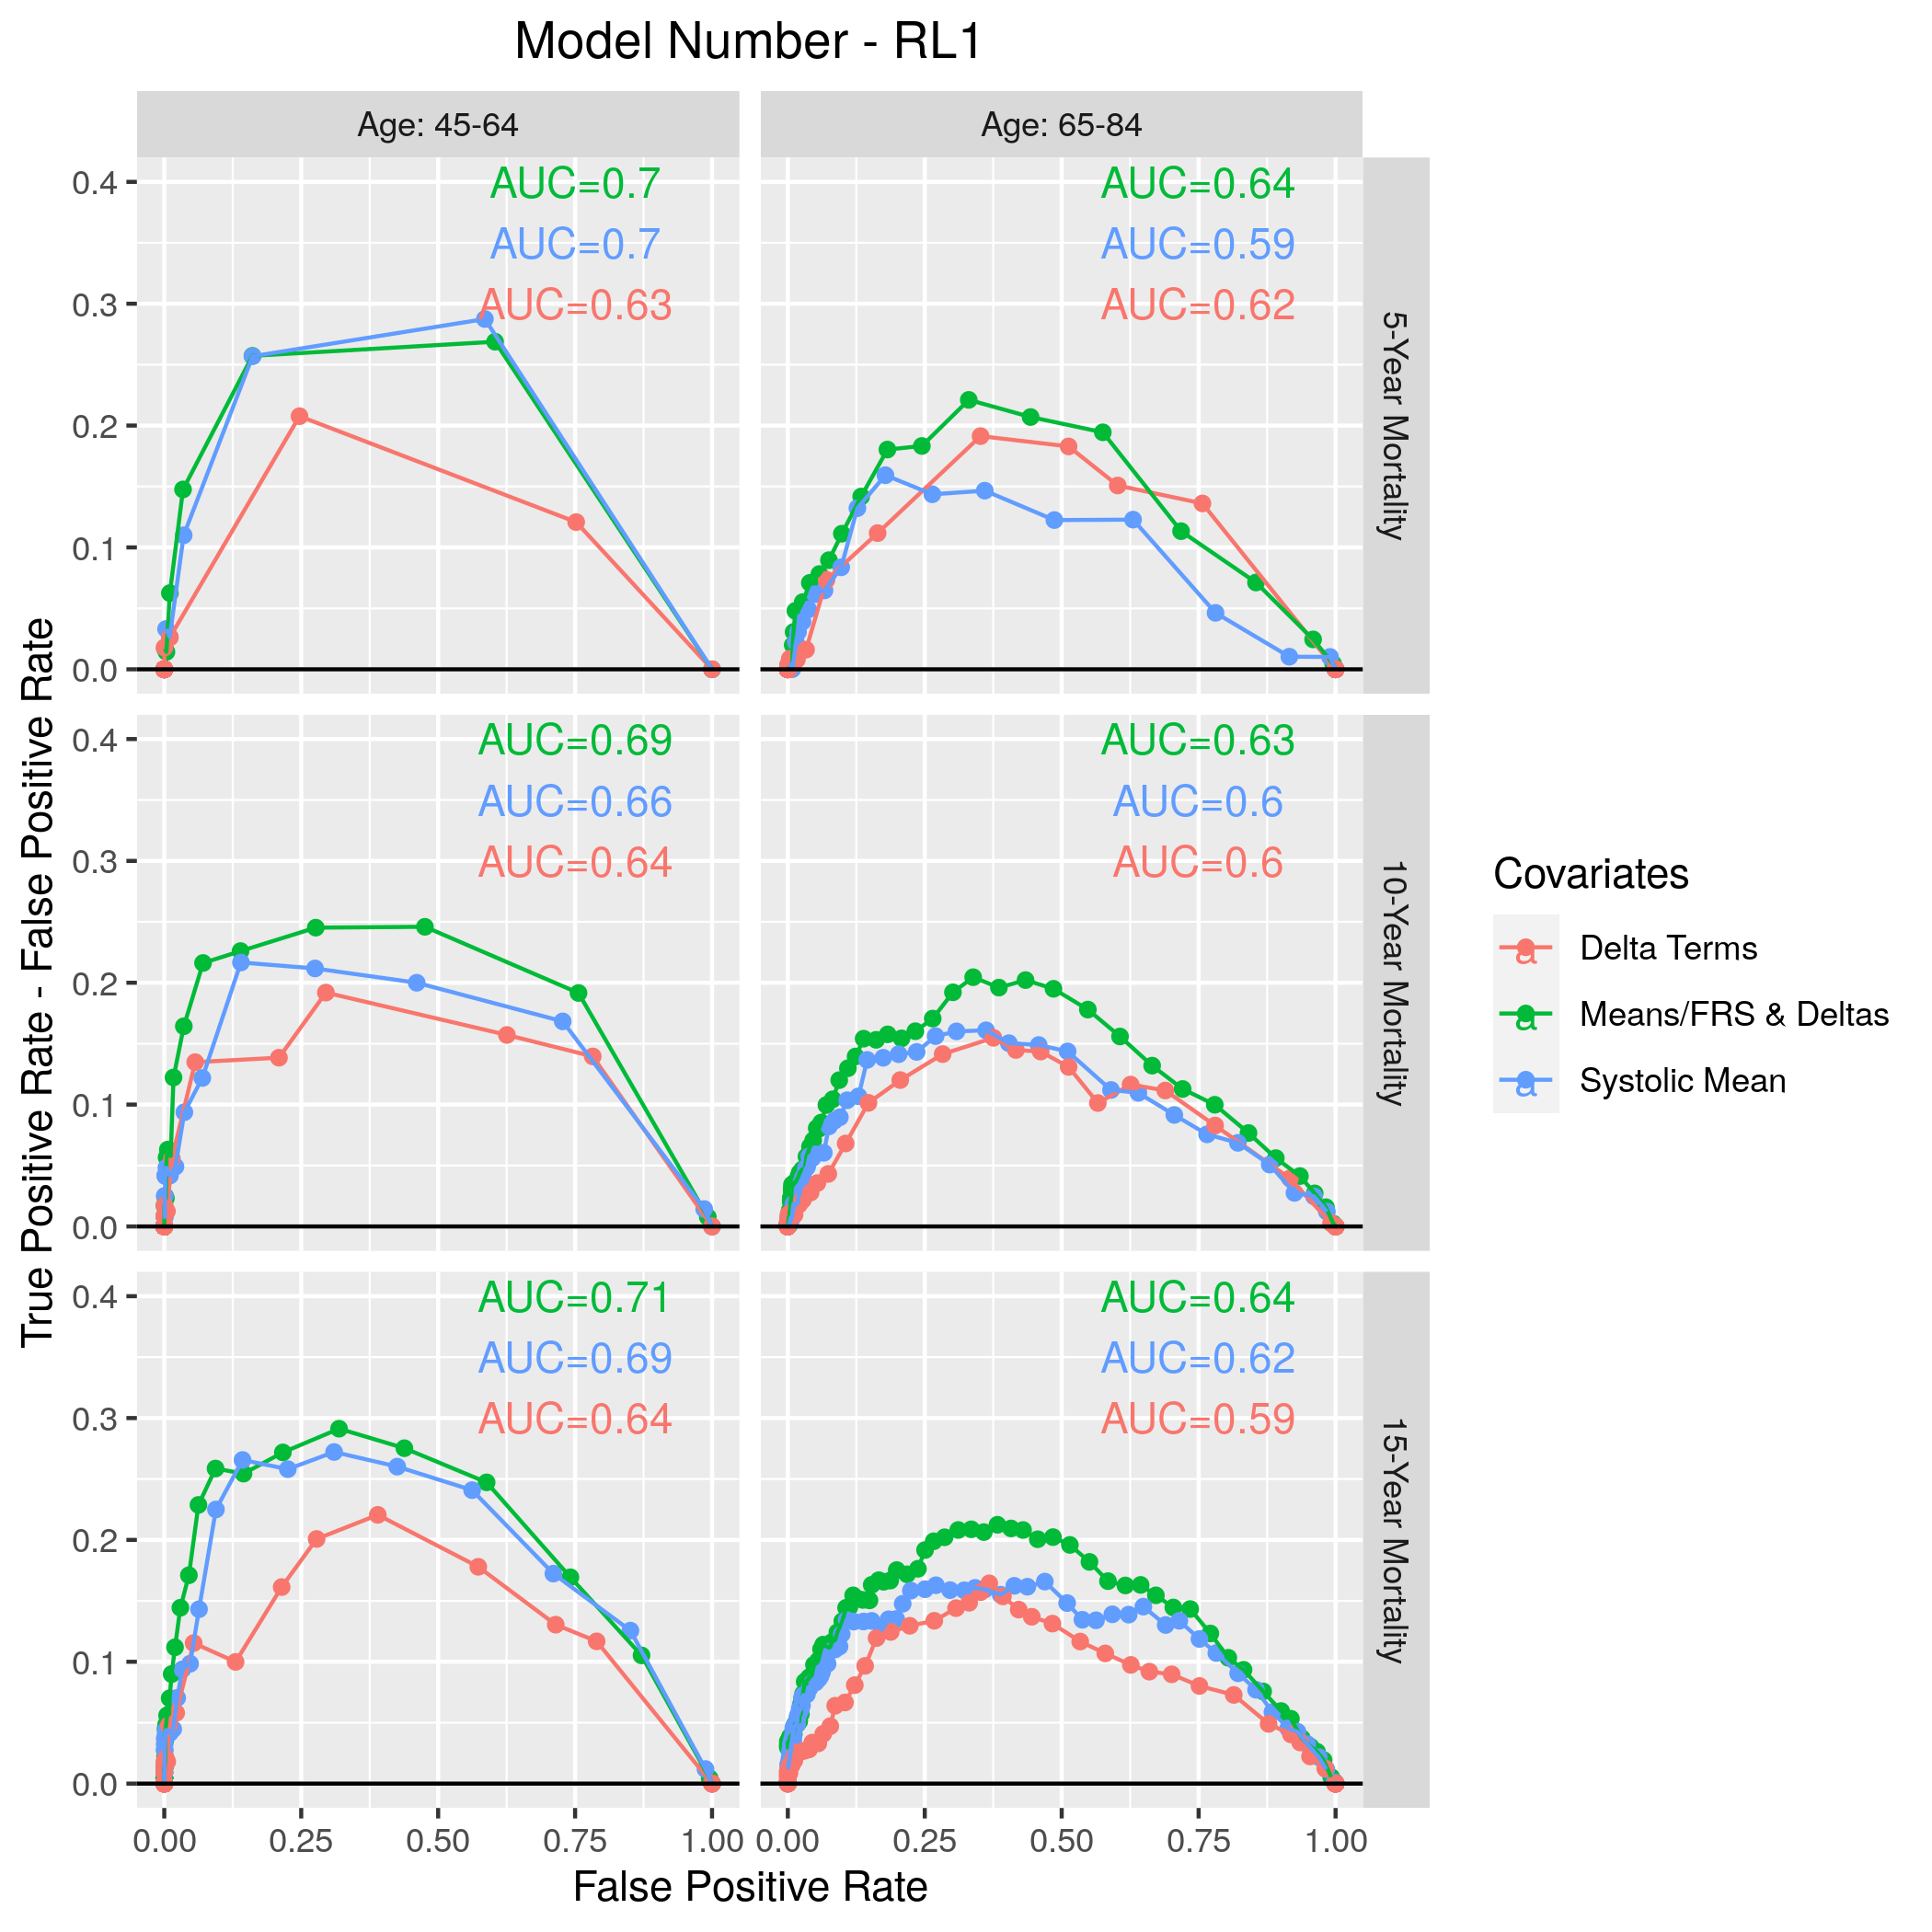
\includegraphics{./Rmarkdown_Plots/ROC_CAx-Covariates_EventType_RL1.png}
\caption{ROC curves for the mean systolic and diastolic model, looking specifically at HA-CVD-CeVD and heart attack-related deaths, stratified by age group and the number of years the survival outcome was predicted since participant starting the survey. The colour of the points and lines represents the different linear predictor covariate models possible.}\label{fig:ROC_RL1}
}
\end{figure}

\begin{figure}
\hypertarget{fig:ROC_RL2}{%
\centering
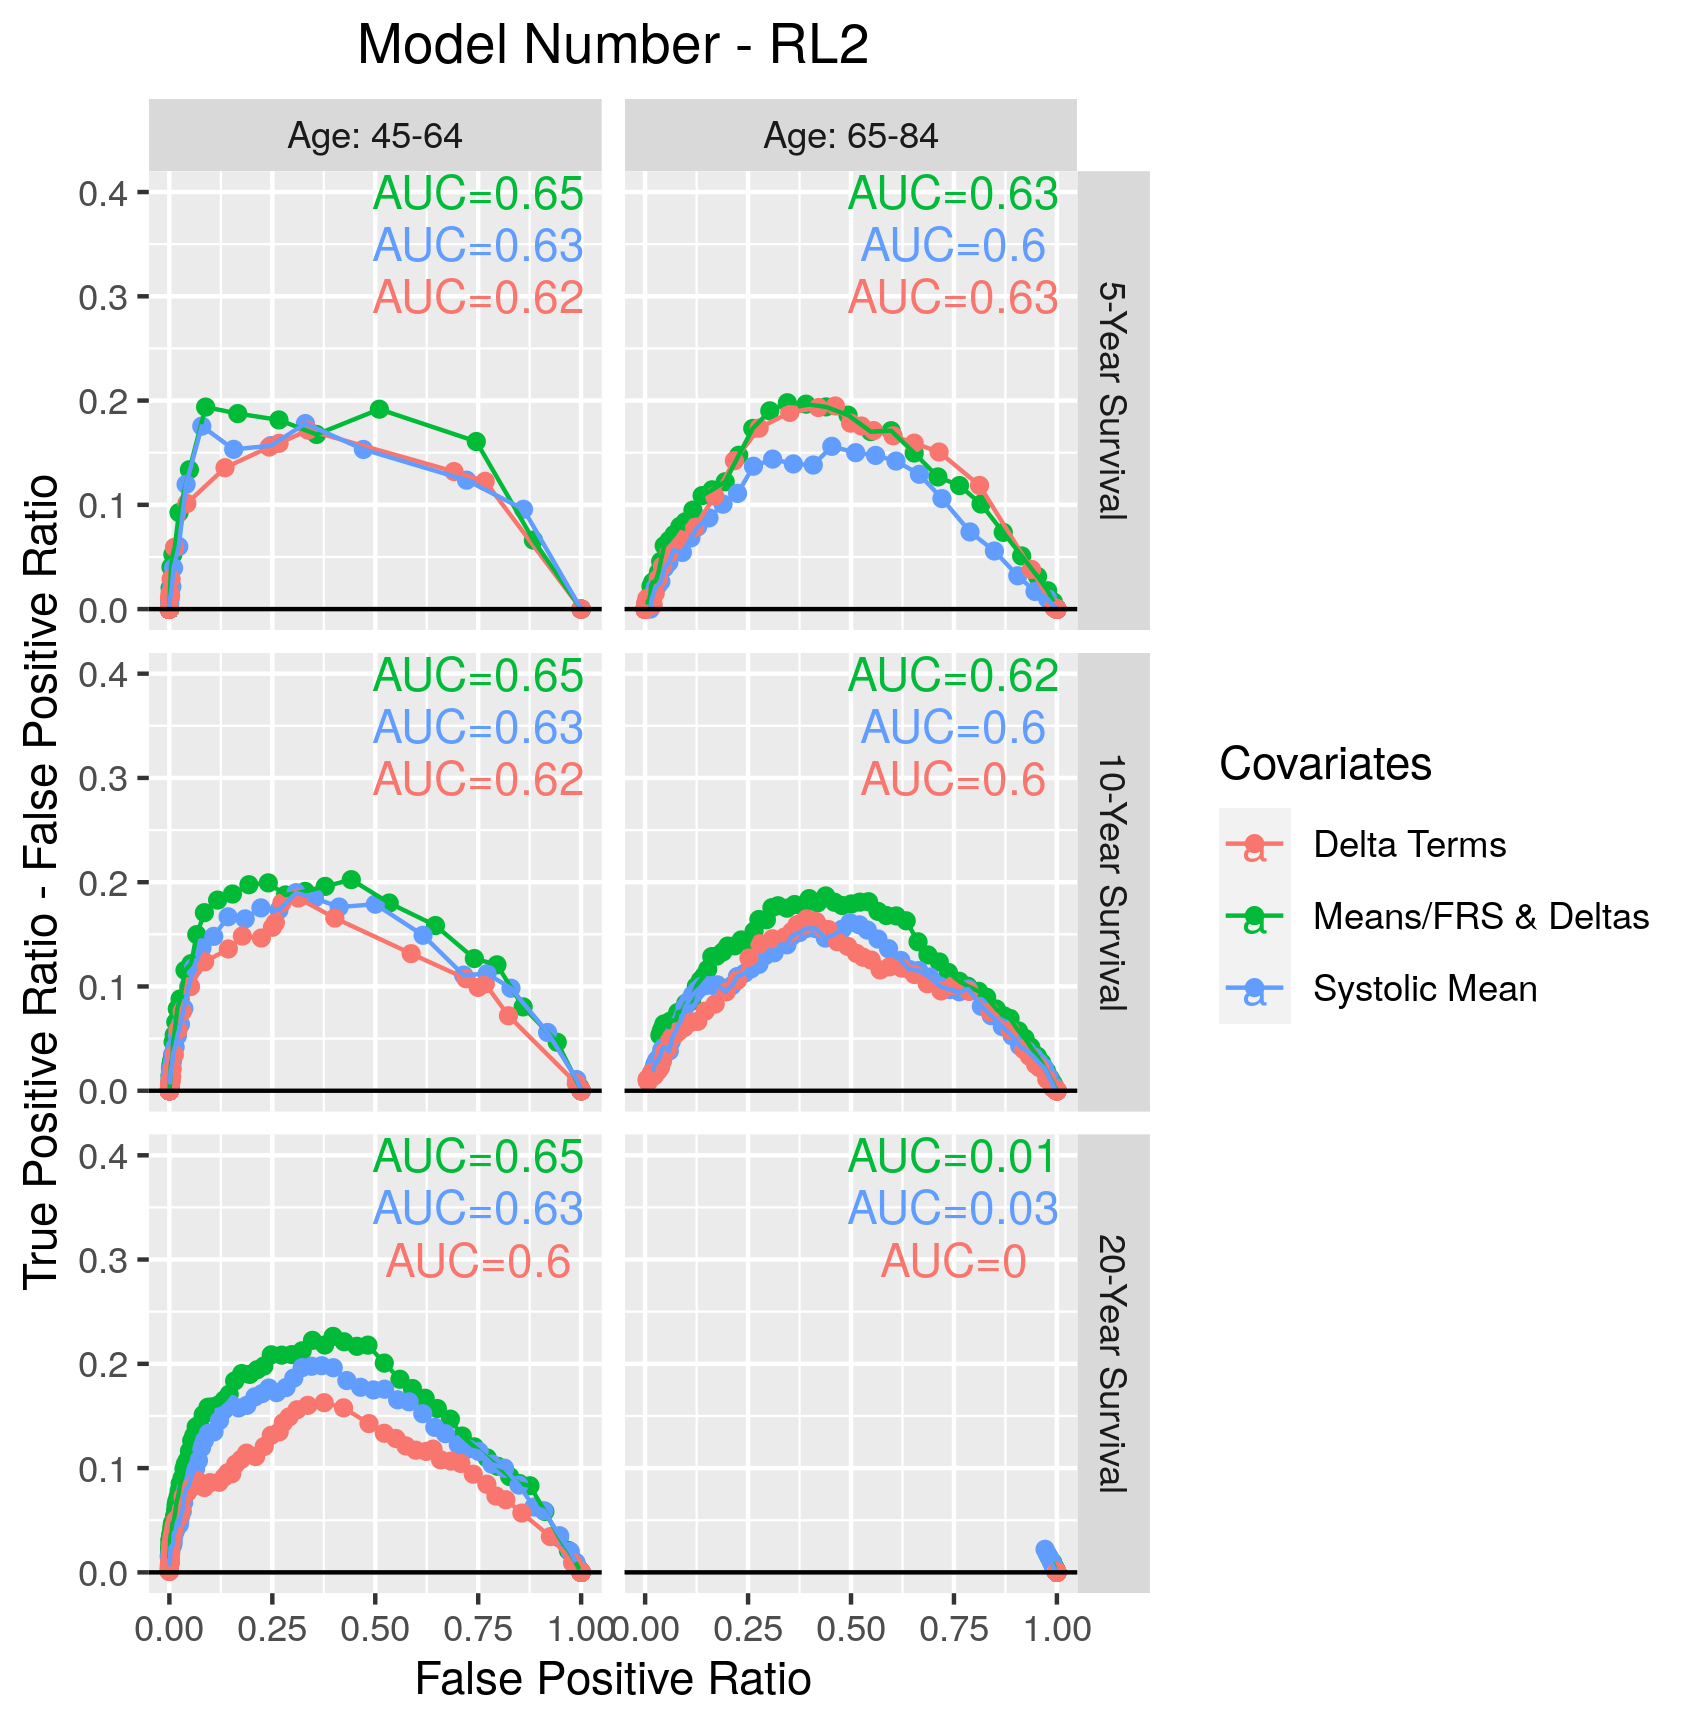
\includegraphics{./Rmarkdown_Plots/ROC_CAx-Covariates_EventType_RL2.png}
\caption{ROC curves for the mean systolic and diastolic model, looking at all-cause deaths, stratified by age group and the number of years the survival outcome was predicted since participant starting the survey. The colour of the points and lines represents the different linear predictor covariate models possible.}\label{fig:ROC_RL2}
}
\end{figure}

\begin{figure}
\hypertarget{fig:ROC_RL2oth}{%
\centering
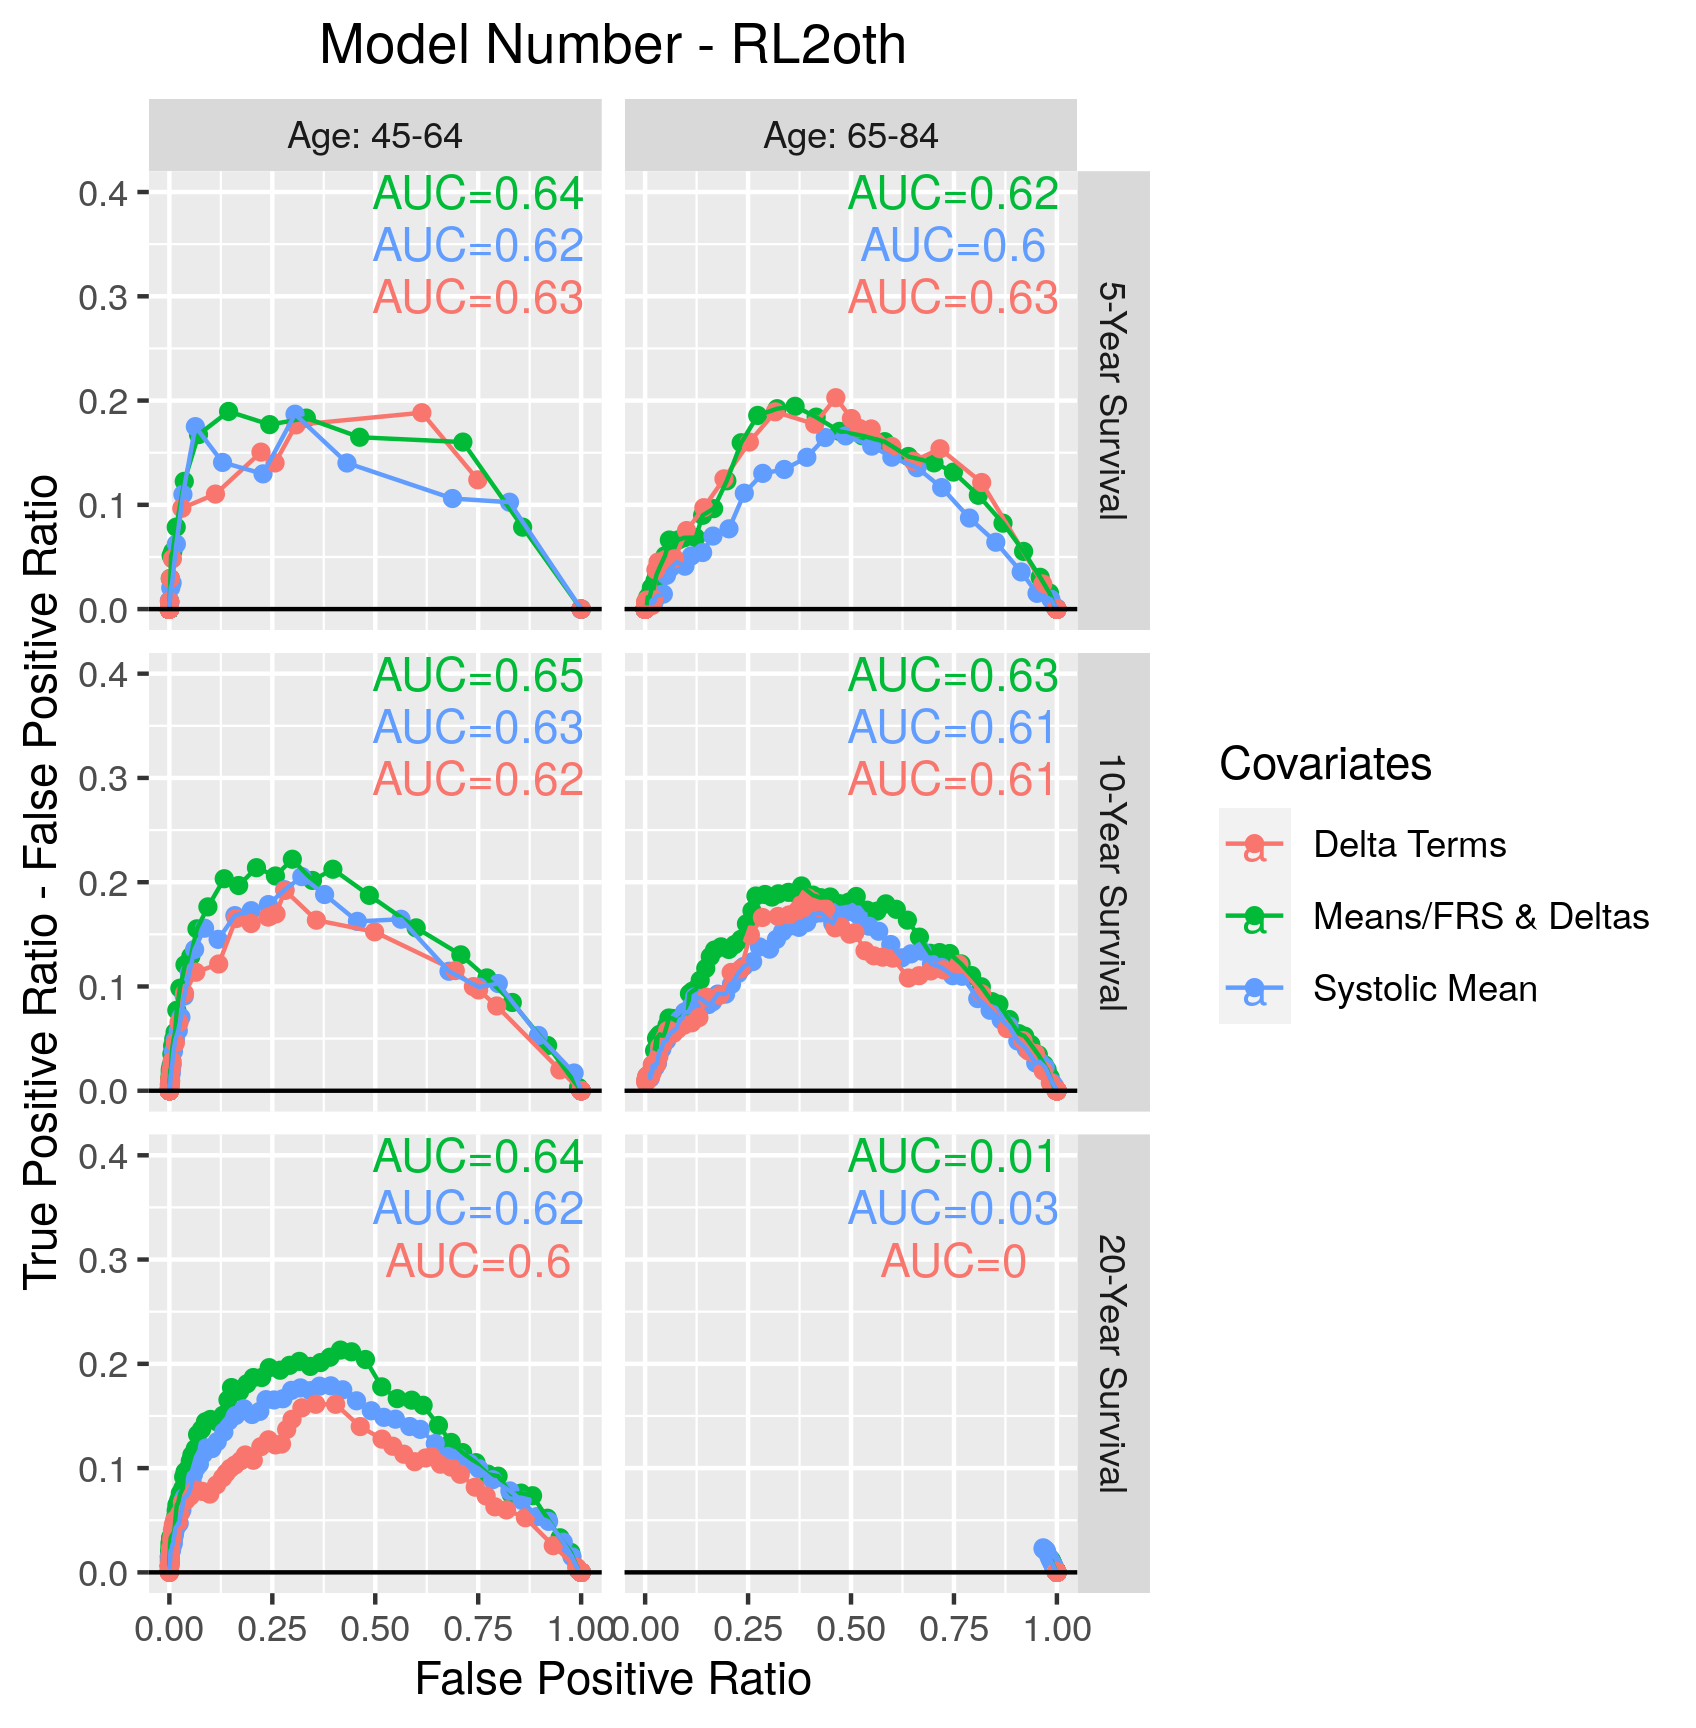
\includegraphics{./Rmarkdown_Plots/ROC_CAx-Covariates_EventType_RL2oth.png}
\caption{ROC curves for the mean systolic and diastolic model, looking non-HA-CVD-CeVD and heart attack-related deaths, stratified by age group and the number of years the survival outcome was predicted since participant starting the survey. The colour of the points and lines represents the different linear predictor covariate models possible.}\label{fig:ROC_RL2oth}
}
\end{figure}

\begin{figure}
\hypertarget{fig:ROC_RL7}{%
\centering
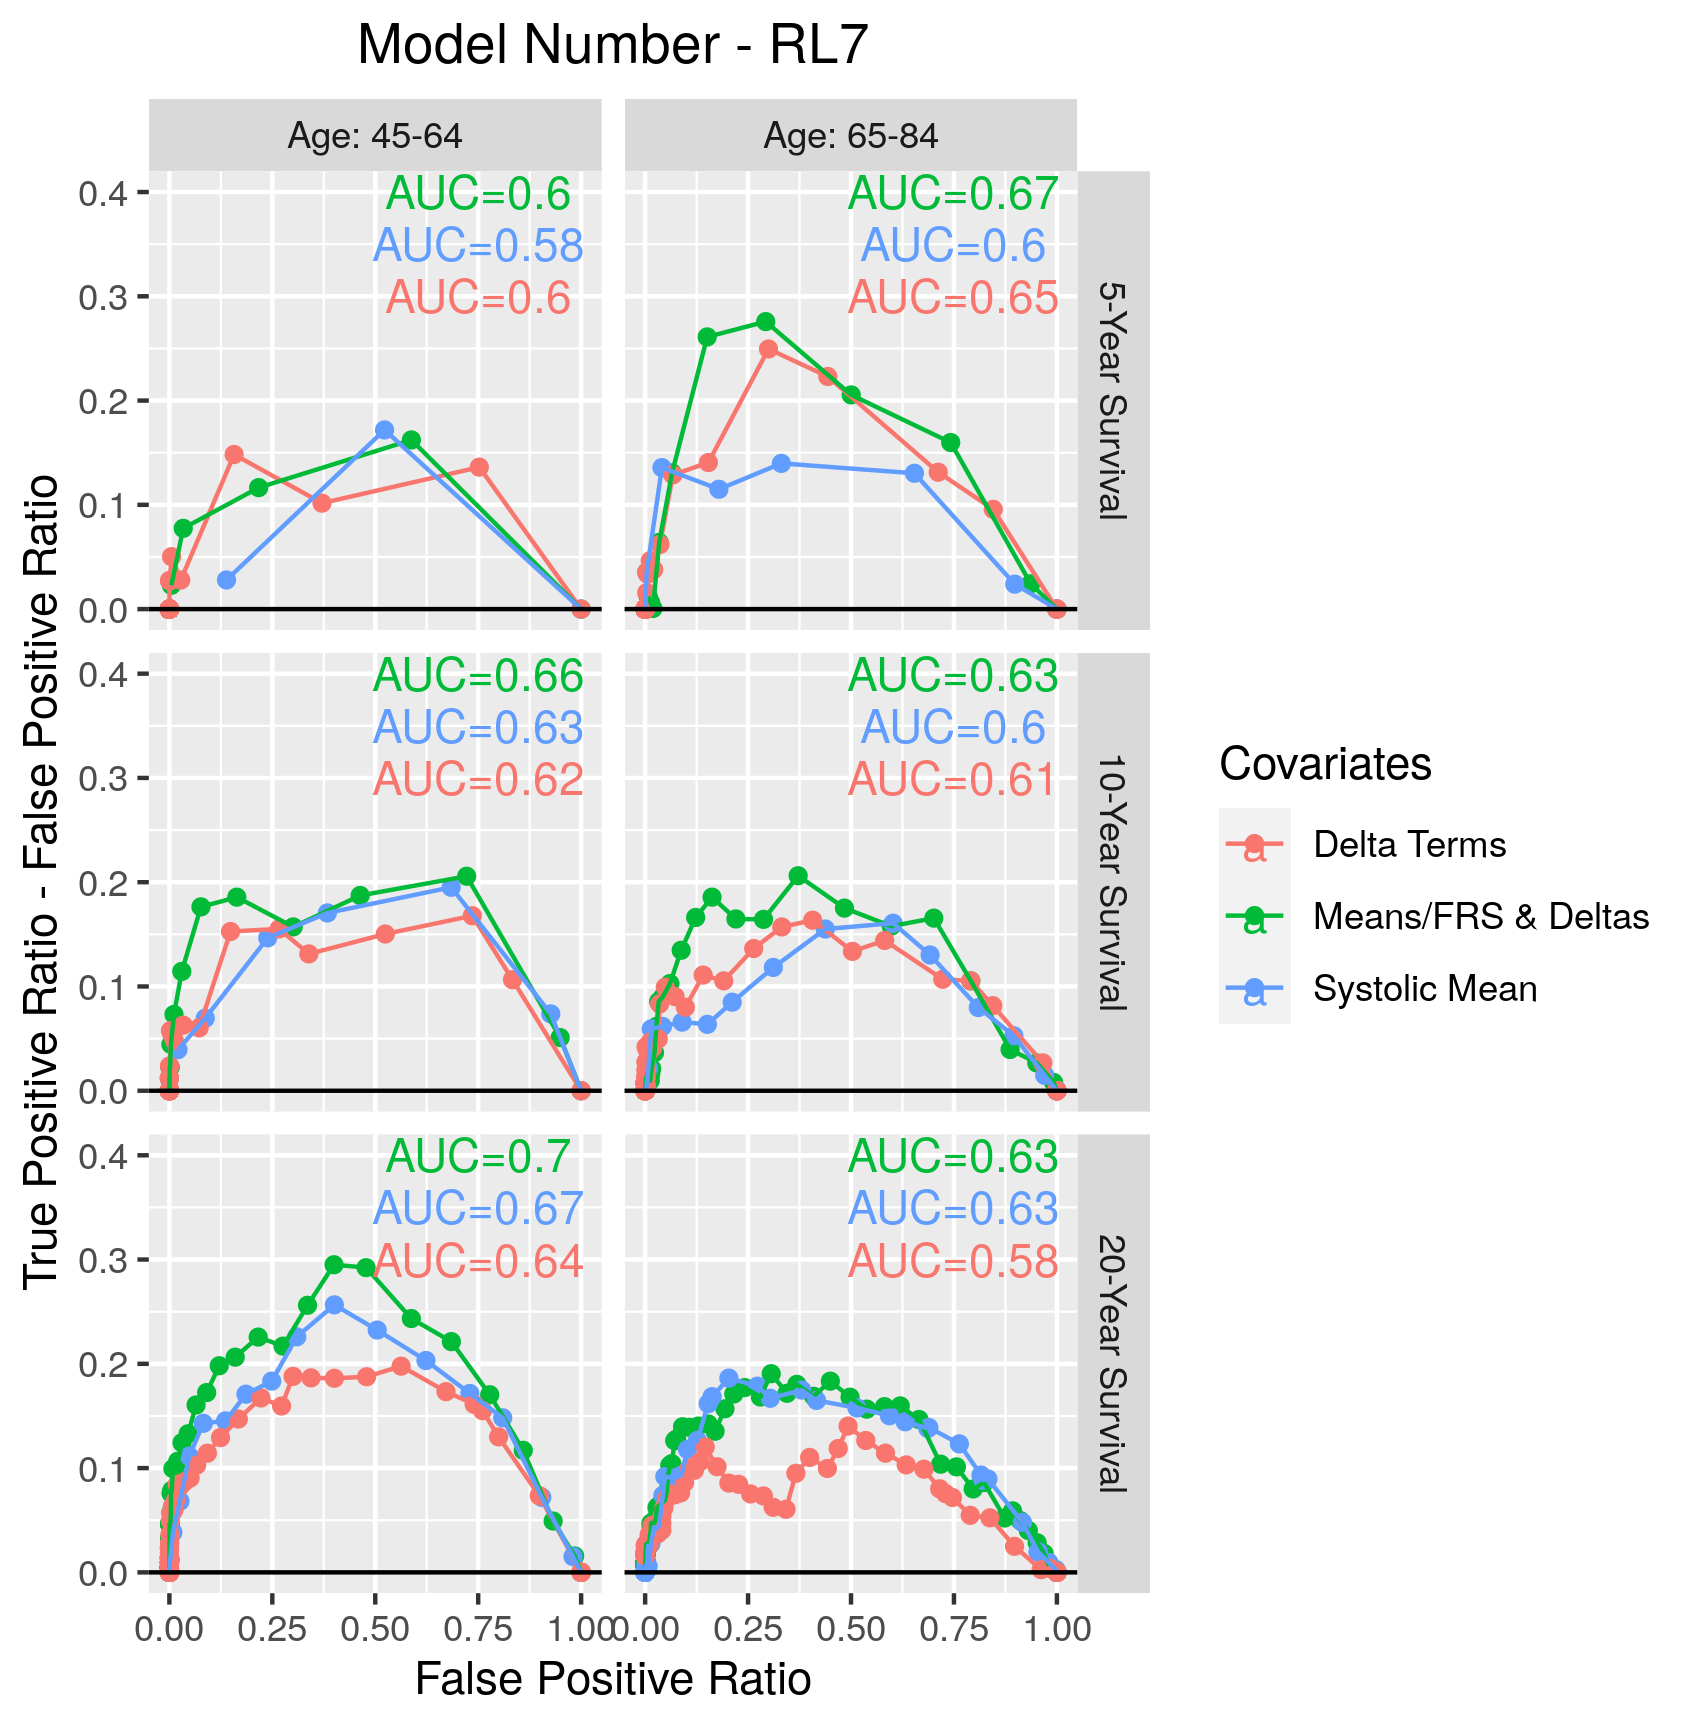
\includegraphics{./Rmarkdown_Plots/ROC_CAx-Covariates_EventType_RL7.png}
\caption{ROC curves for for the FRS-based model, looking specifically at HA-CVD-CeVD and heart attack-related deaths, stratified by age group and the number of years the survival outcome was predicted since participant starting the survey. The colour of the points and lines represents the different linear predictor covariate models possible.}\label{fig:ROC_RL7}
}
\end{figure}

\begin{figure}
\hypertarget{fig:ROC_RL8}{%
\centering
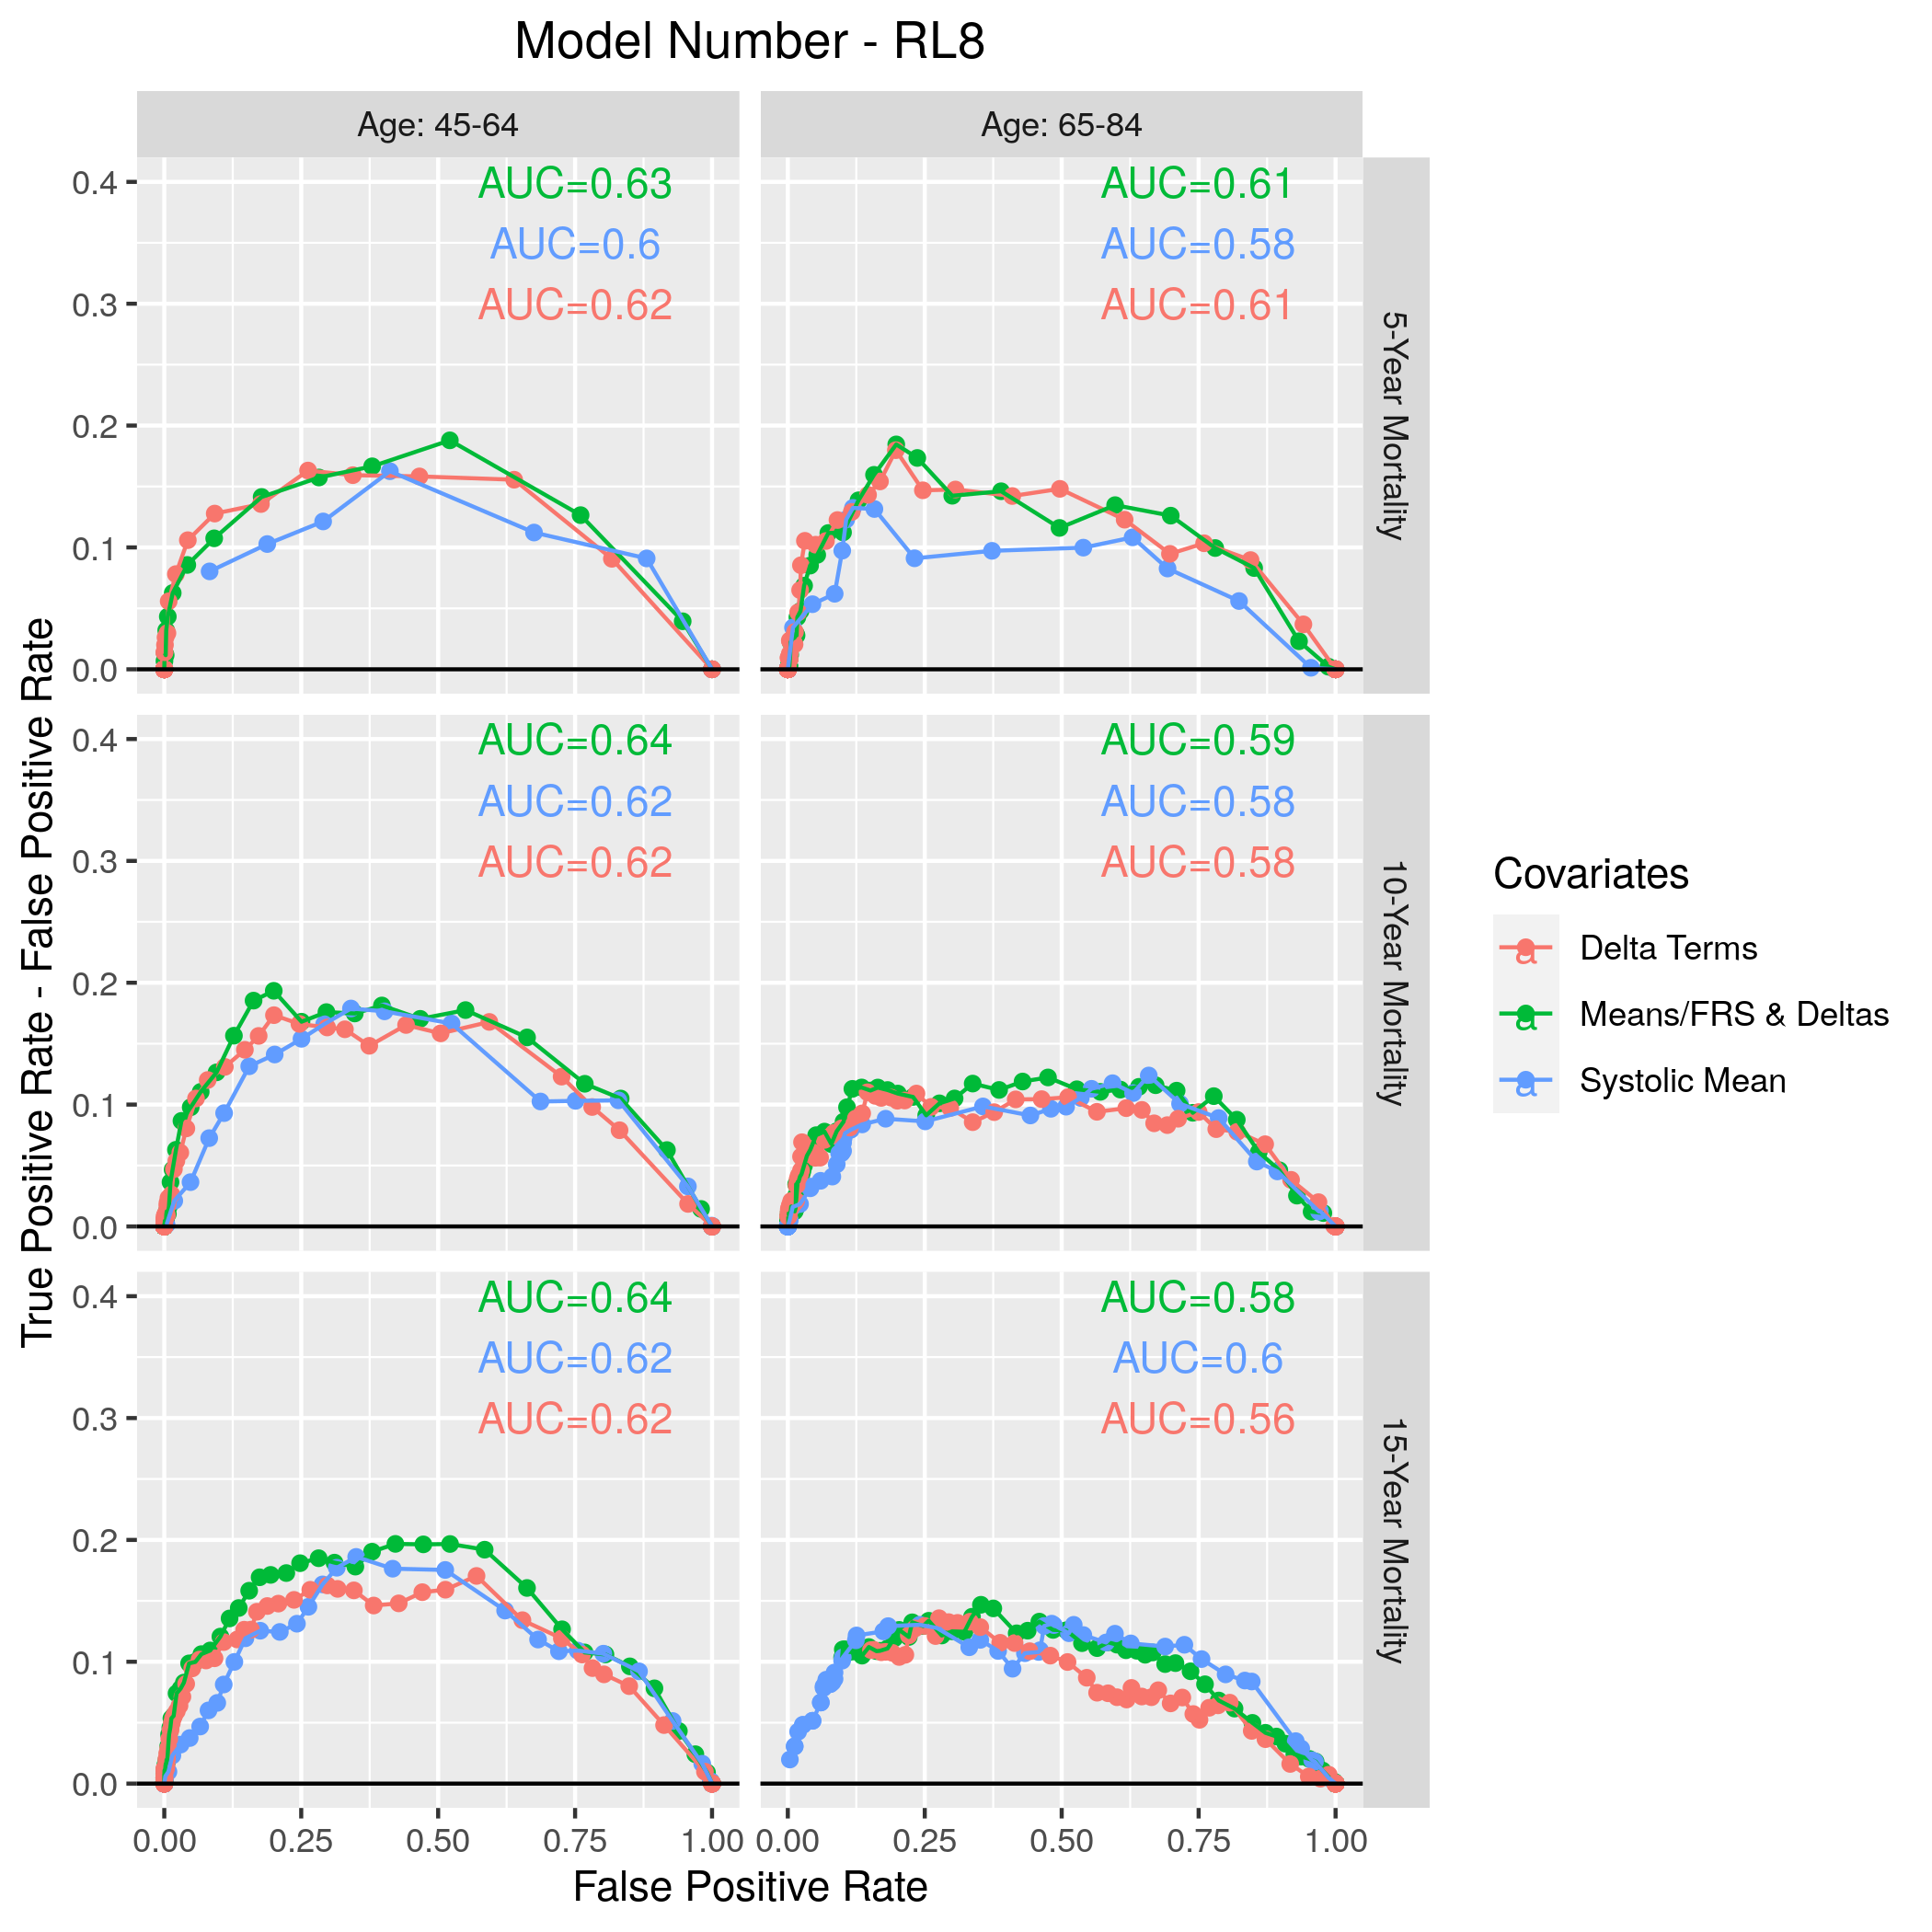
\includegraphics{./Rmarkdown_Plots/ROC_CAx-Covariates_EventType_RL8.png}
\caption{ROC curves for for the FRS-based model, looking at all-cause deaths, stratified by age group and the number of years the survival outcome was predicted since participant starting the survey. The colour of the points and lines represents the different linear predictor covariate models possible.}\label{fig:ROC_RL8}
}
\end{figure}

\begin{figure}
\hypertarget{fig:ROC_RL8oth}{%
\centering
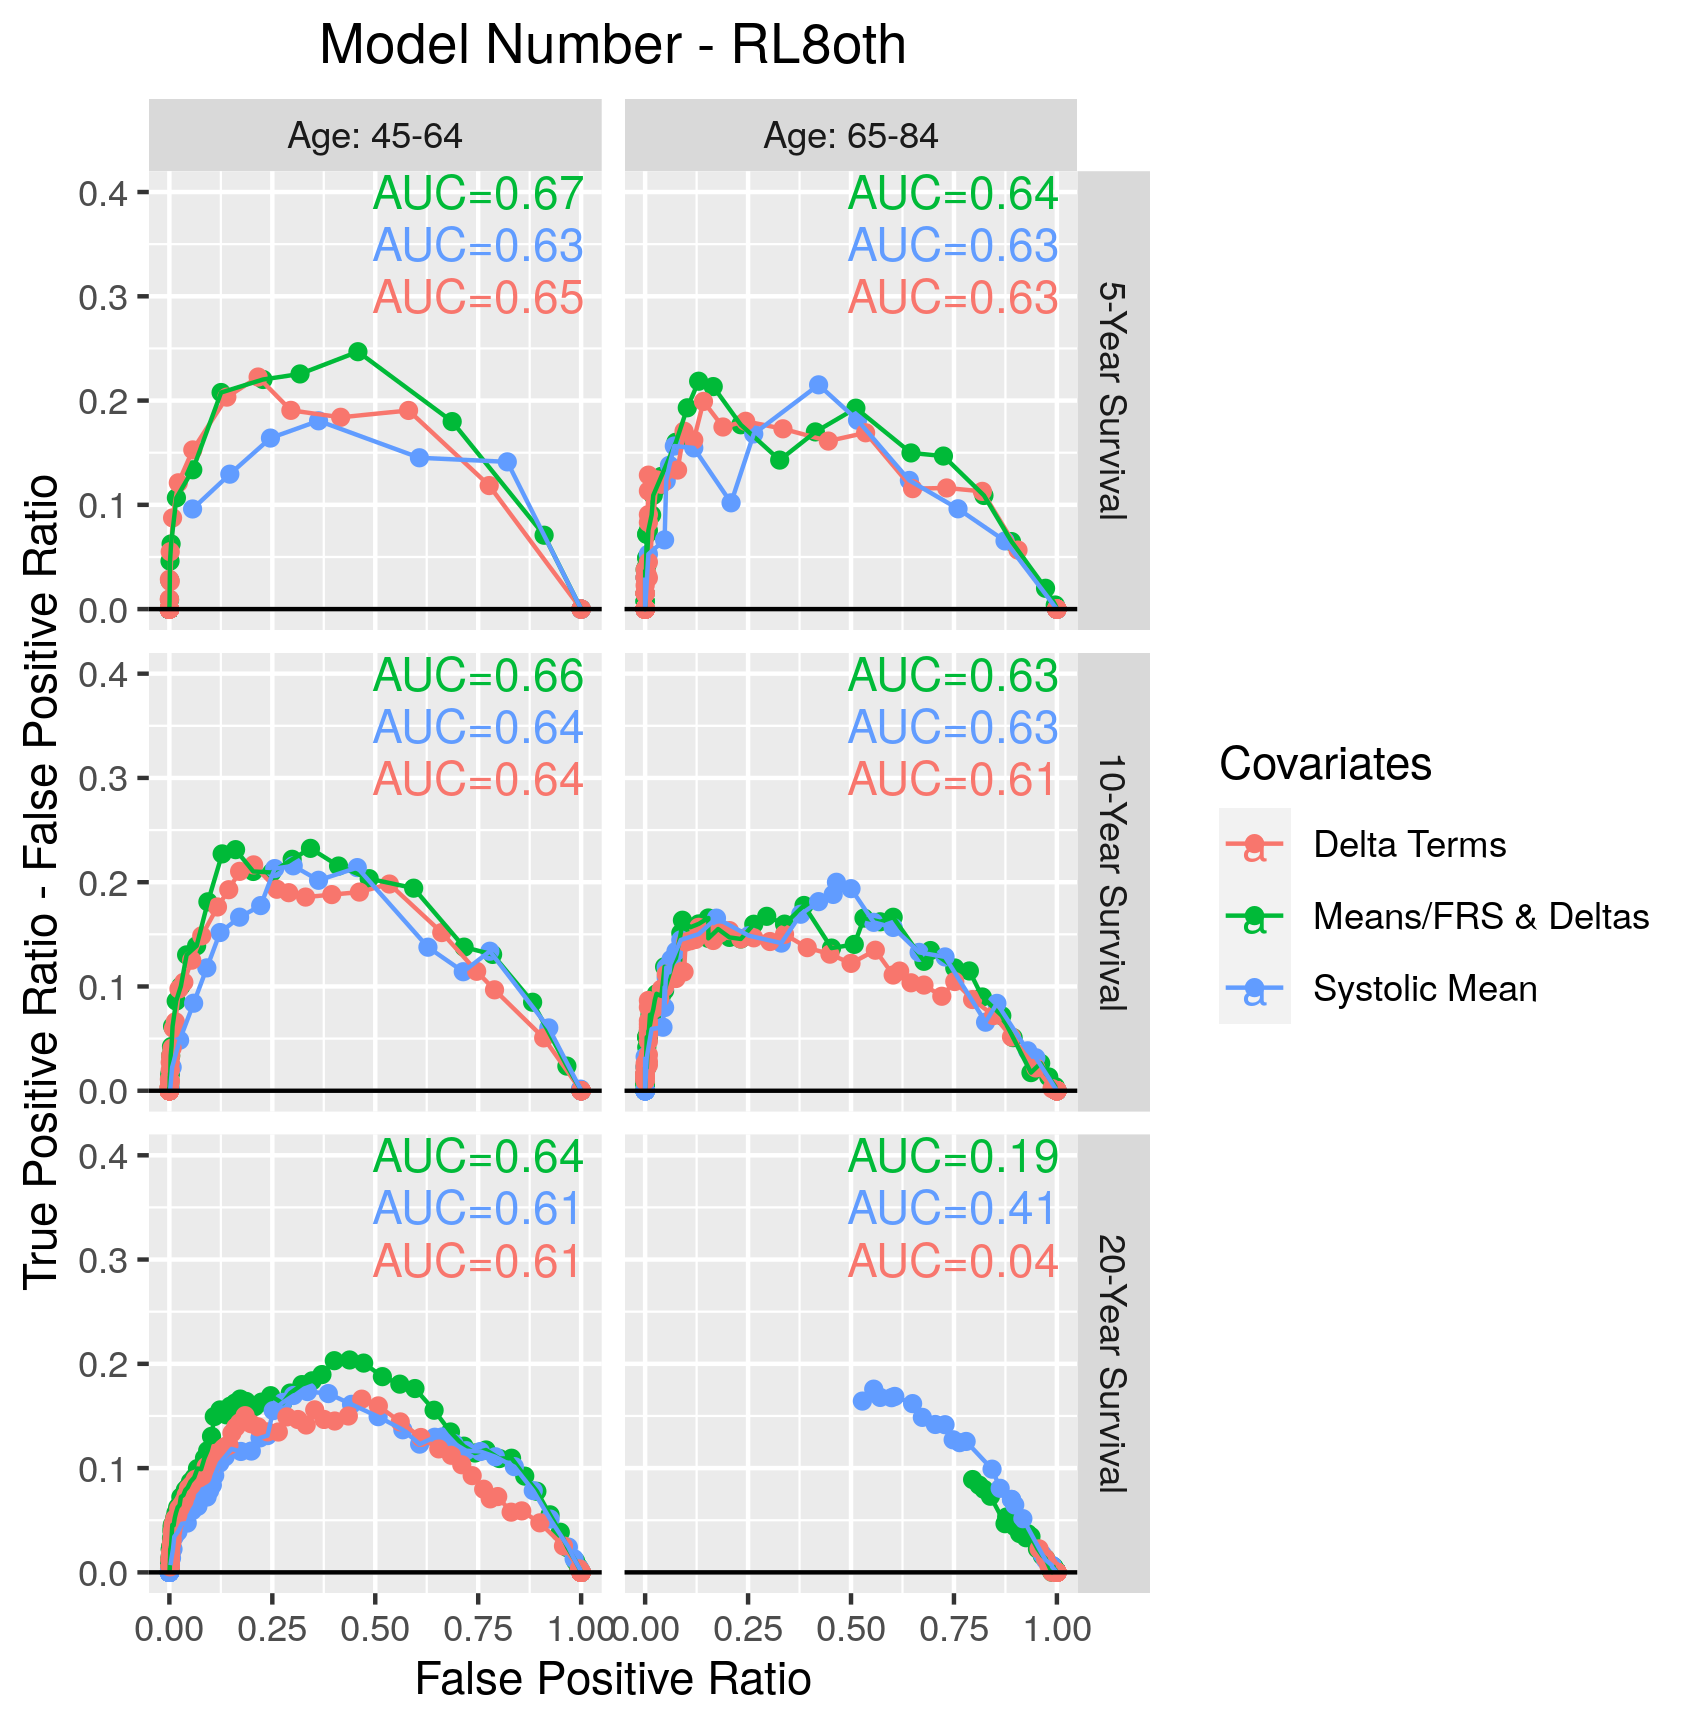
\includegraphics{./Rmarkdown_Plots/ROC_CAx-Covariates_EventType_RL8oth.png}
\caption{ROC curves for for the FRS-based model, looking non-HA-CVD-CeVD and heart attack-related deaths, stratified by age group and the number of years the survival outcome was predicted since participant starting the survey. The colour of the points and lines represents the different linear predictor covariate models possible.}\label{fig:ROC_RL8oth}
}
\end{figure}

\hypertarget{results---exploring-delta-directionality}{%
\subsubsection{\texorpdfstring{Results - Exploring \(\Delta\) Directionality}{Results - Exploring \textbackslash Delta Directionality}}\label{results---exploring-delta-directionality}}

This section of the appendix is to explore whether the directionality of the difference in clinic-home blood pressure (represented through the non-absolute value of the \(\Delta\) covariate) may have an influence on the survival outcome in the population. In the work presented in this article, \(\Delta\) is the absolute value of the differences in the means of the blood pressure measurements at the clinic and at home, respectively, for both diastolic and systolic blood pressure. By `directionality', we refer to whether the difference between the clinic and home mean measurements are positive or negative. Figure \ref{fig:DeltaDensities} shows the clinic-home directionalities, split by demographic group, indicating no significant difference between the different demographic groups. There is a general trend that the directionality for systolic and diastolic blood pressure is more likely to be the same than opposite.

\begin{figure}
\hypertarget{fig:DeltaDensities}{%
\centering
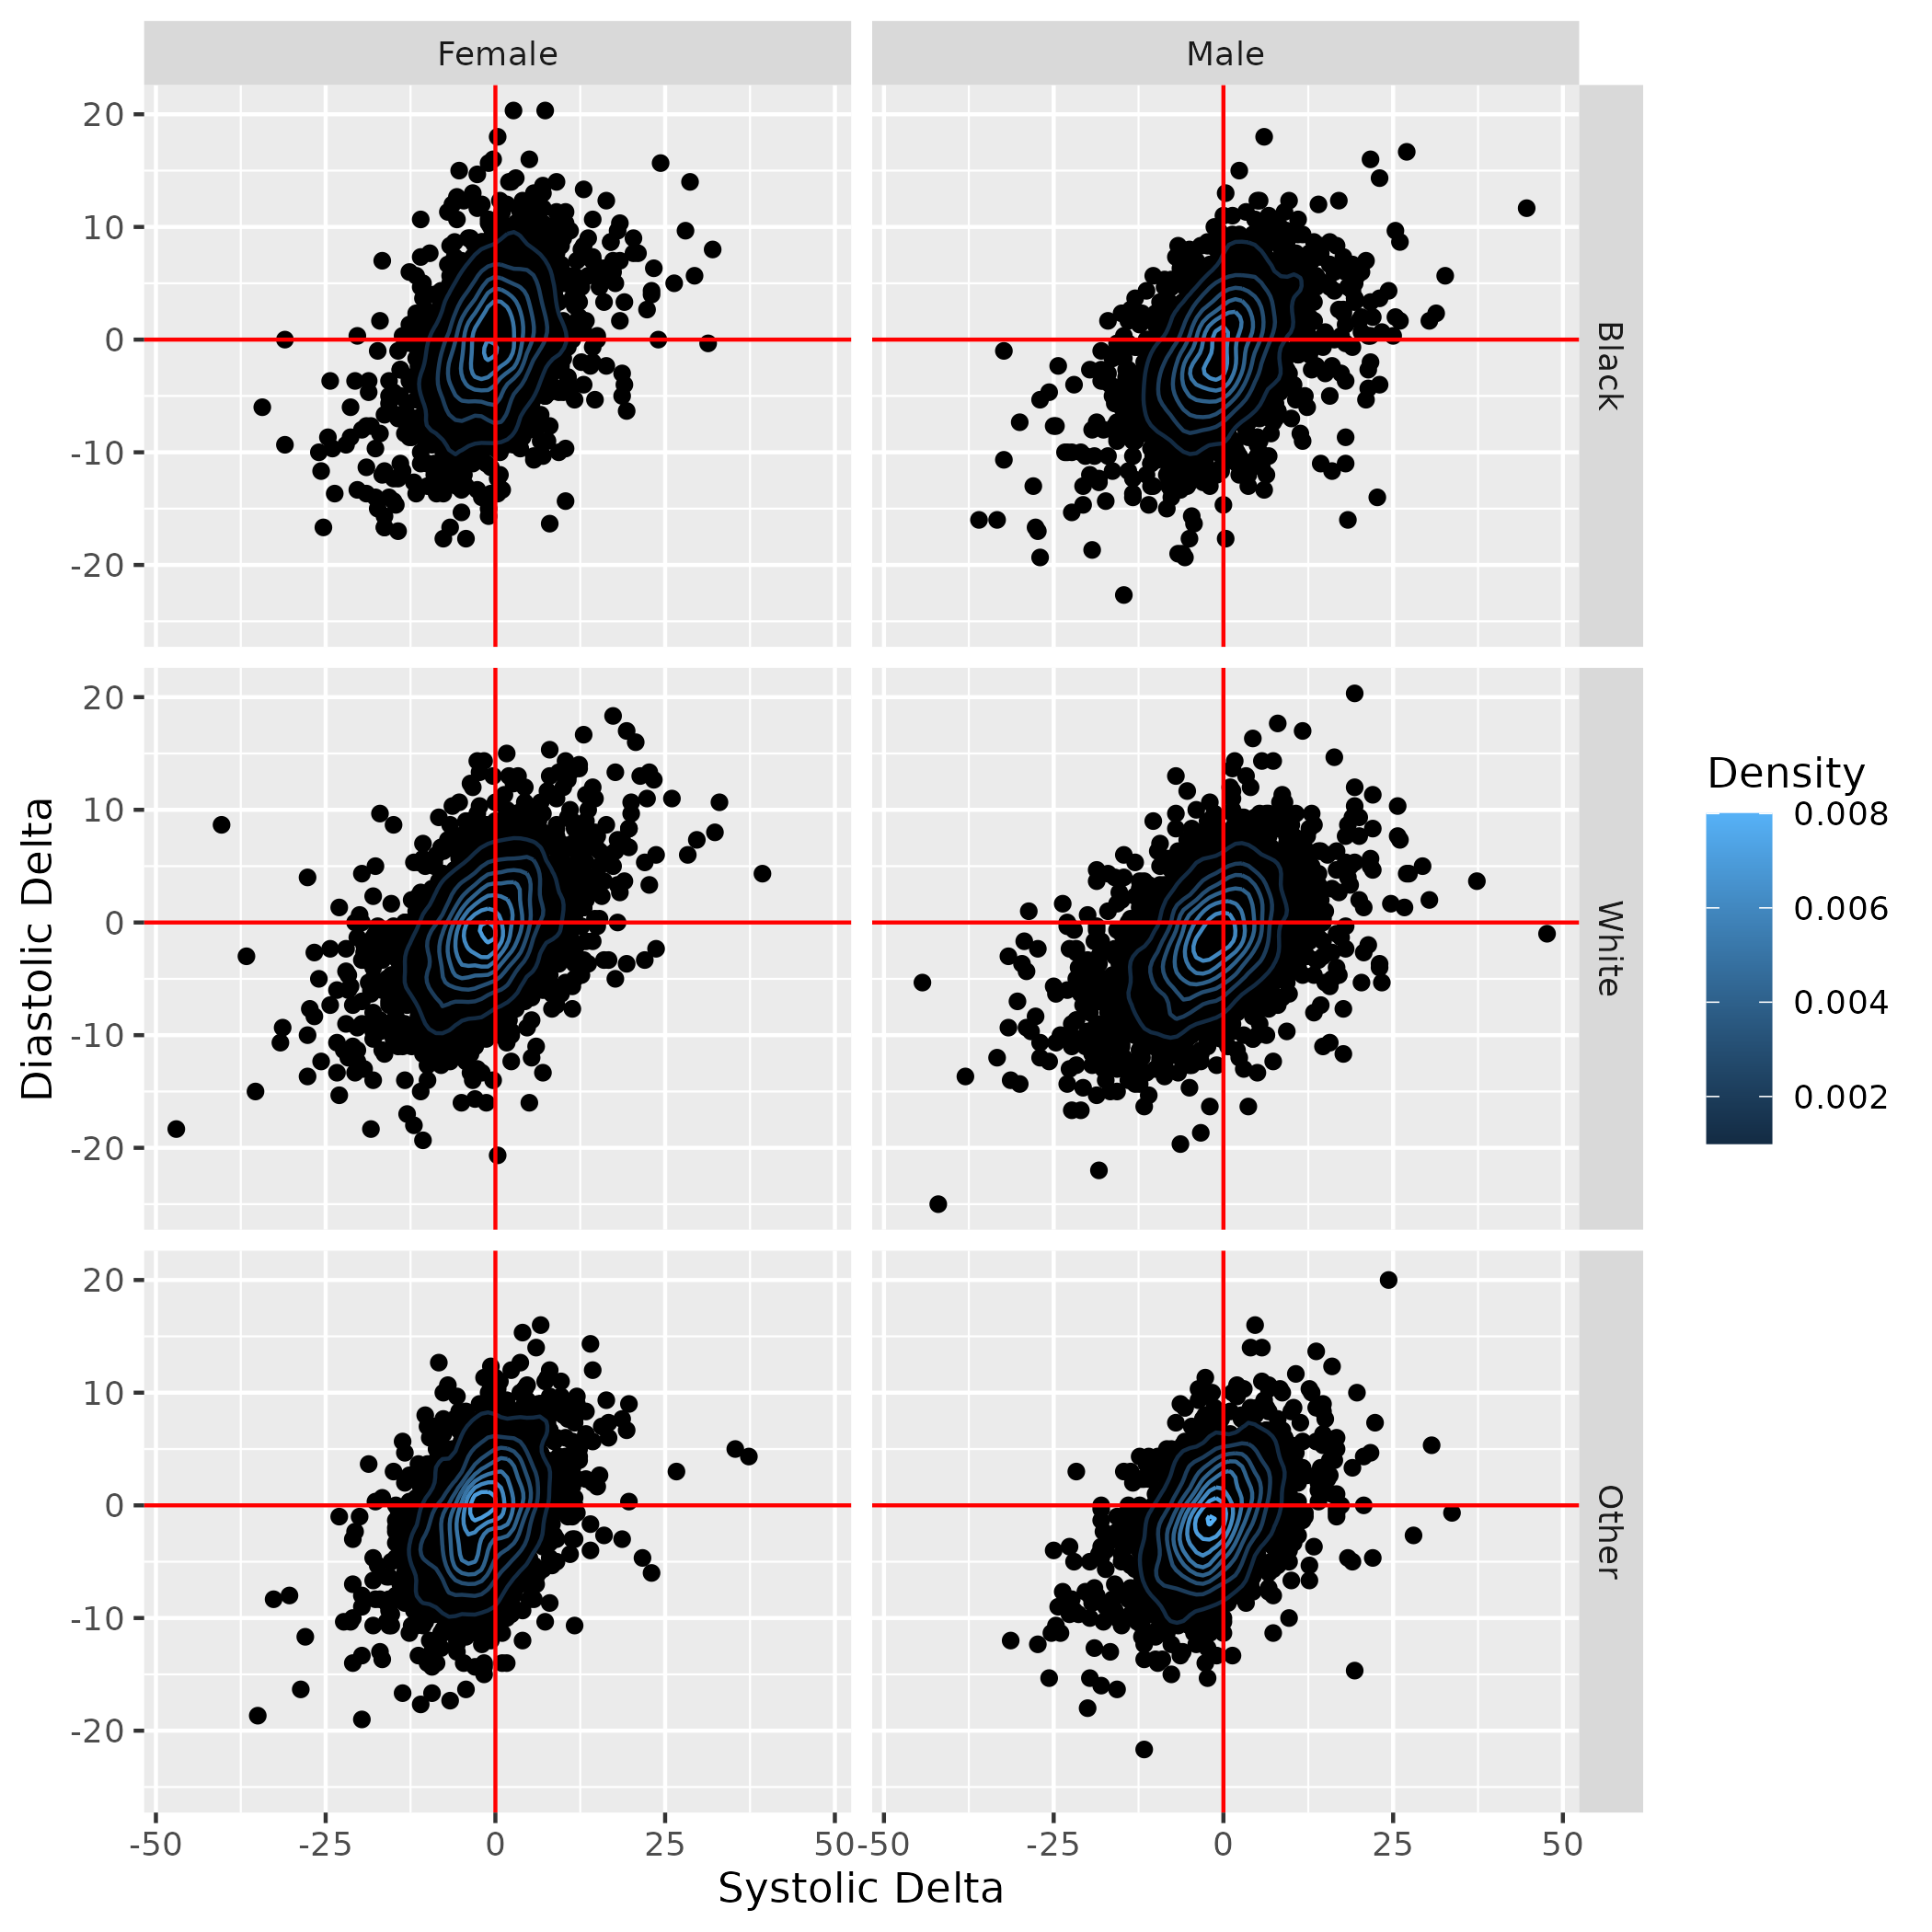
\includegraphics{./Rmarkdown_Plots/Delta_plusminus_Demography.png}
\caption{The range of the non-absolute \(\Delta\) values in the systolic and diastolic blood pressure measurements, split by demographic group. This reflects the differences between the average measurements at the clinic and at home.}\label{fig:DeltaDensities}
}
\end{figure}

In order to explore whether the directionality of the clinic-home measurements influences survival outcome, we will use a combination of Kaplan-Meier curves and Cox's proportional hazards regression. The latter will implement a simple Maximum Likelihood Estimation (MLE) method based on summary statistics of the Bayesian posterior blood pressure values, not the Bayesian-HMC method applied elsewhere in this article. The Kaplan-Meier curve is a plot of the change in survival probability of a population in time since the start of a survey/census. The survival distribution is calculated using
\begin{equation}\label{survKM}
\hat{S}(t)=\prod_{t_j \le t}\left(1-\frac{d_j}{r_j} \right),
\end{equation}
for \(d_j\) the number of individuals who die within the time interval \(t_j\) and \(r_j\) the population that are alive (at risk of death) and not censored. Greenwood's formula is used to calculate the variance of the Kaplan-Meier estimation
\begin{equation}\label{sigKM}
\hat{\sigma}(t)^2=\hat{S}(t)^2\sum_{t_j \le t}\left(\frac{d_j}{r_j(r_j-d_j)} \right).
\end{equation}
The 100(1-\(\alpha\))\% confidence intervals of the Kaplan-Meier estimate are assumed to be normally distributed
\begin{equation}\label{CIKM}
\hat{S}(t) \pm z_{1-\alpha/2}\hat{\sigma}(t).
\end{equation}

Figures \ref{fig:KM45tot} and \ref{fig:KM65tot} show the Kaplan-Meier estimates for the full NHANES population for HA-CVD-CeVD mortality, split by demographic group, for the age range 45-64 and 65-84, respectively. The survival probability of the older population decreases faster in time than the middle-aged (45-64) population.

\begin{figure}
\hypertarget{fig:KM45tot}{%
\centering
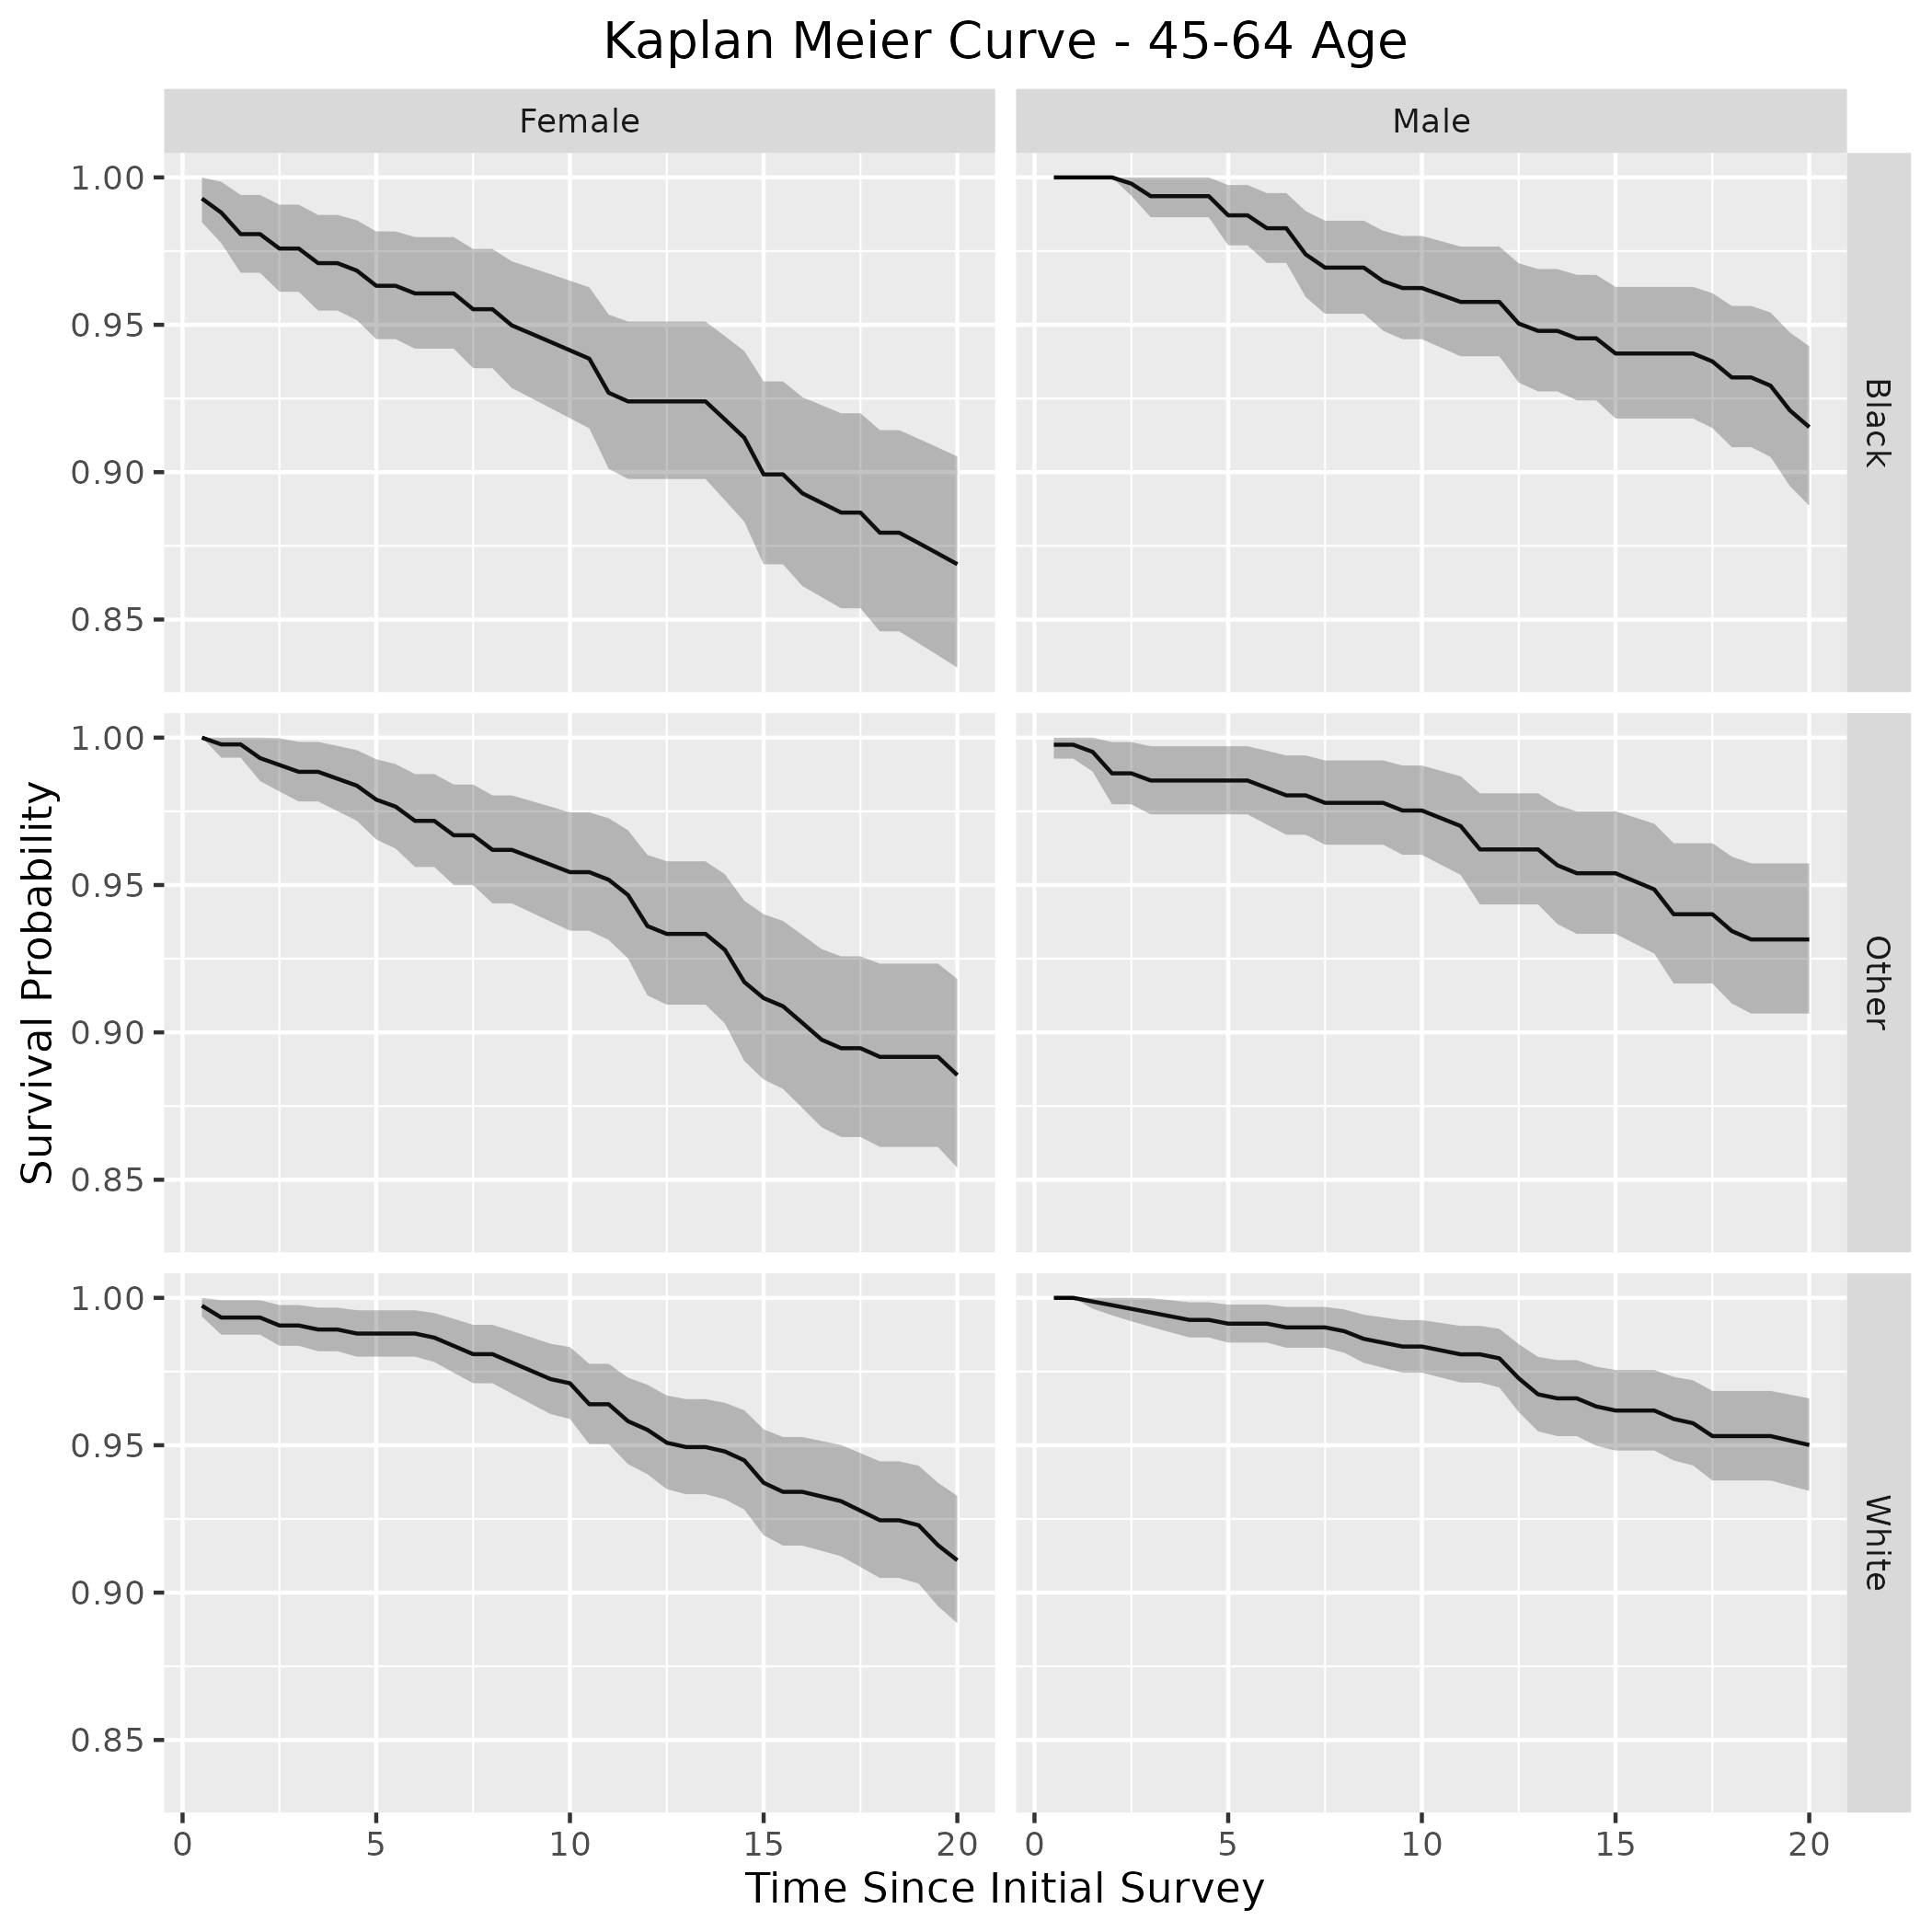
\includegraphics{./Rmarkdown_Plots/SurvProbKM_45-64.png}
\caption{Kaplan-Meier plots of the full-population for HA-CVD-CeVD mortality, for ages between 45-64, split by demographic group.}\label{fig:KM45tot}
}
\end{figure}

\begin{figure}
\hypertarget{fig:KM65tot}{%
\centering
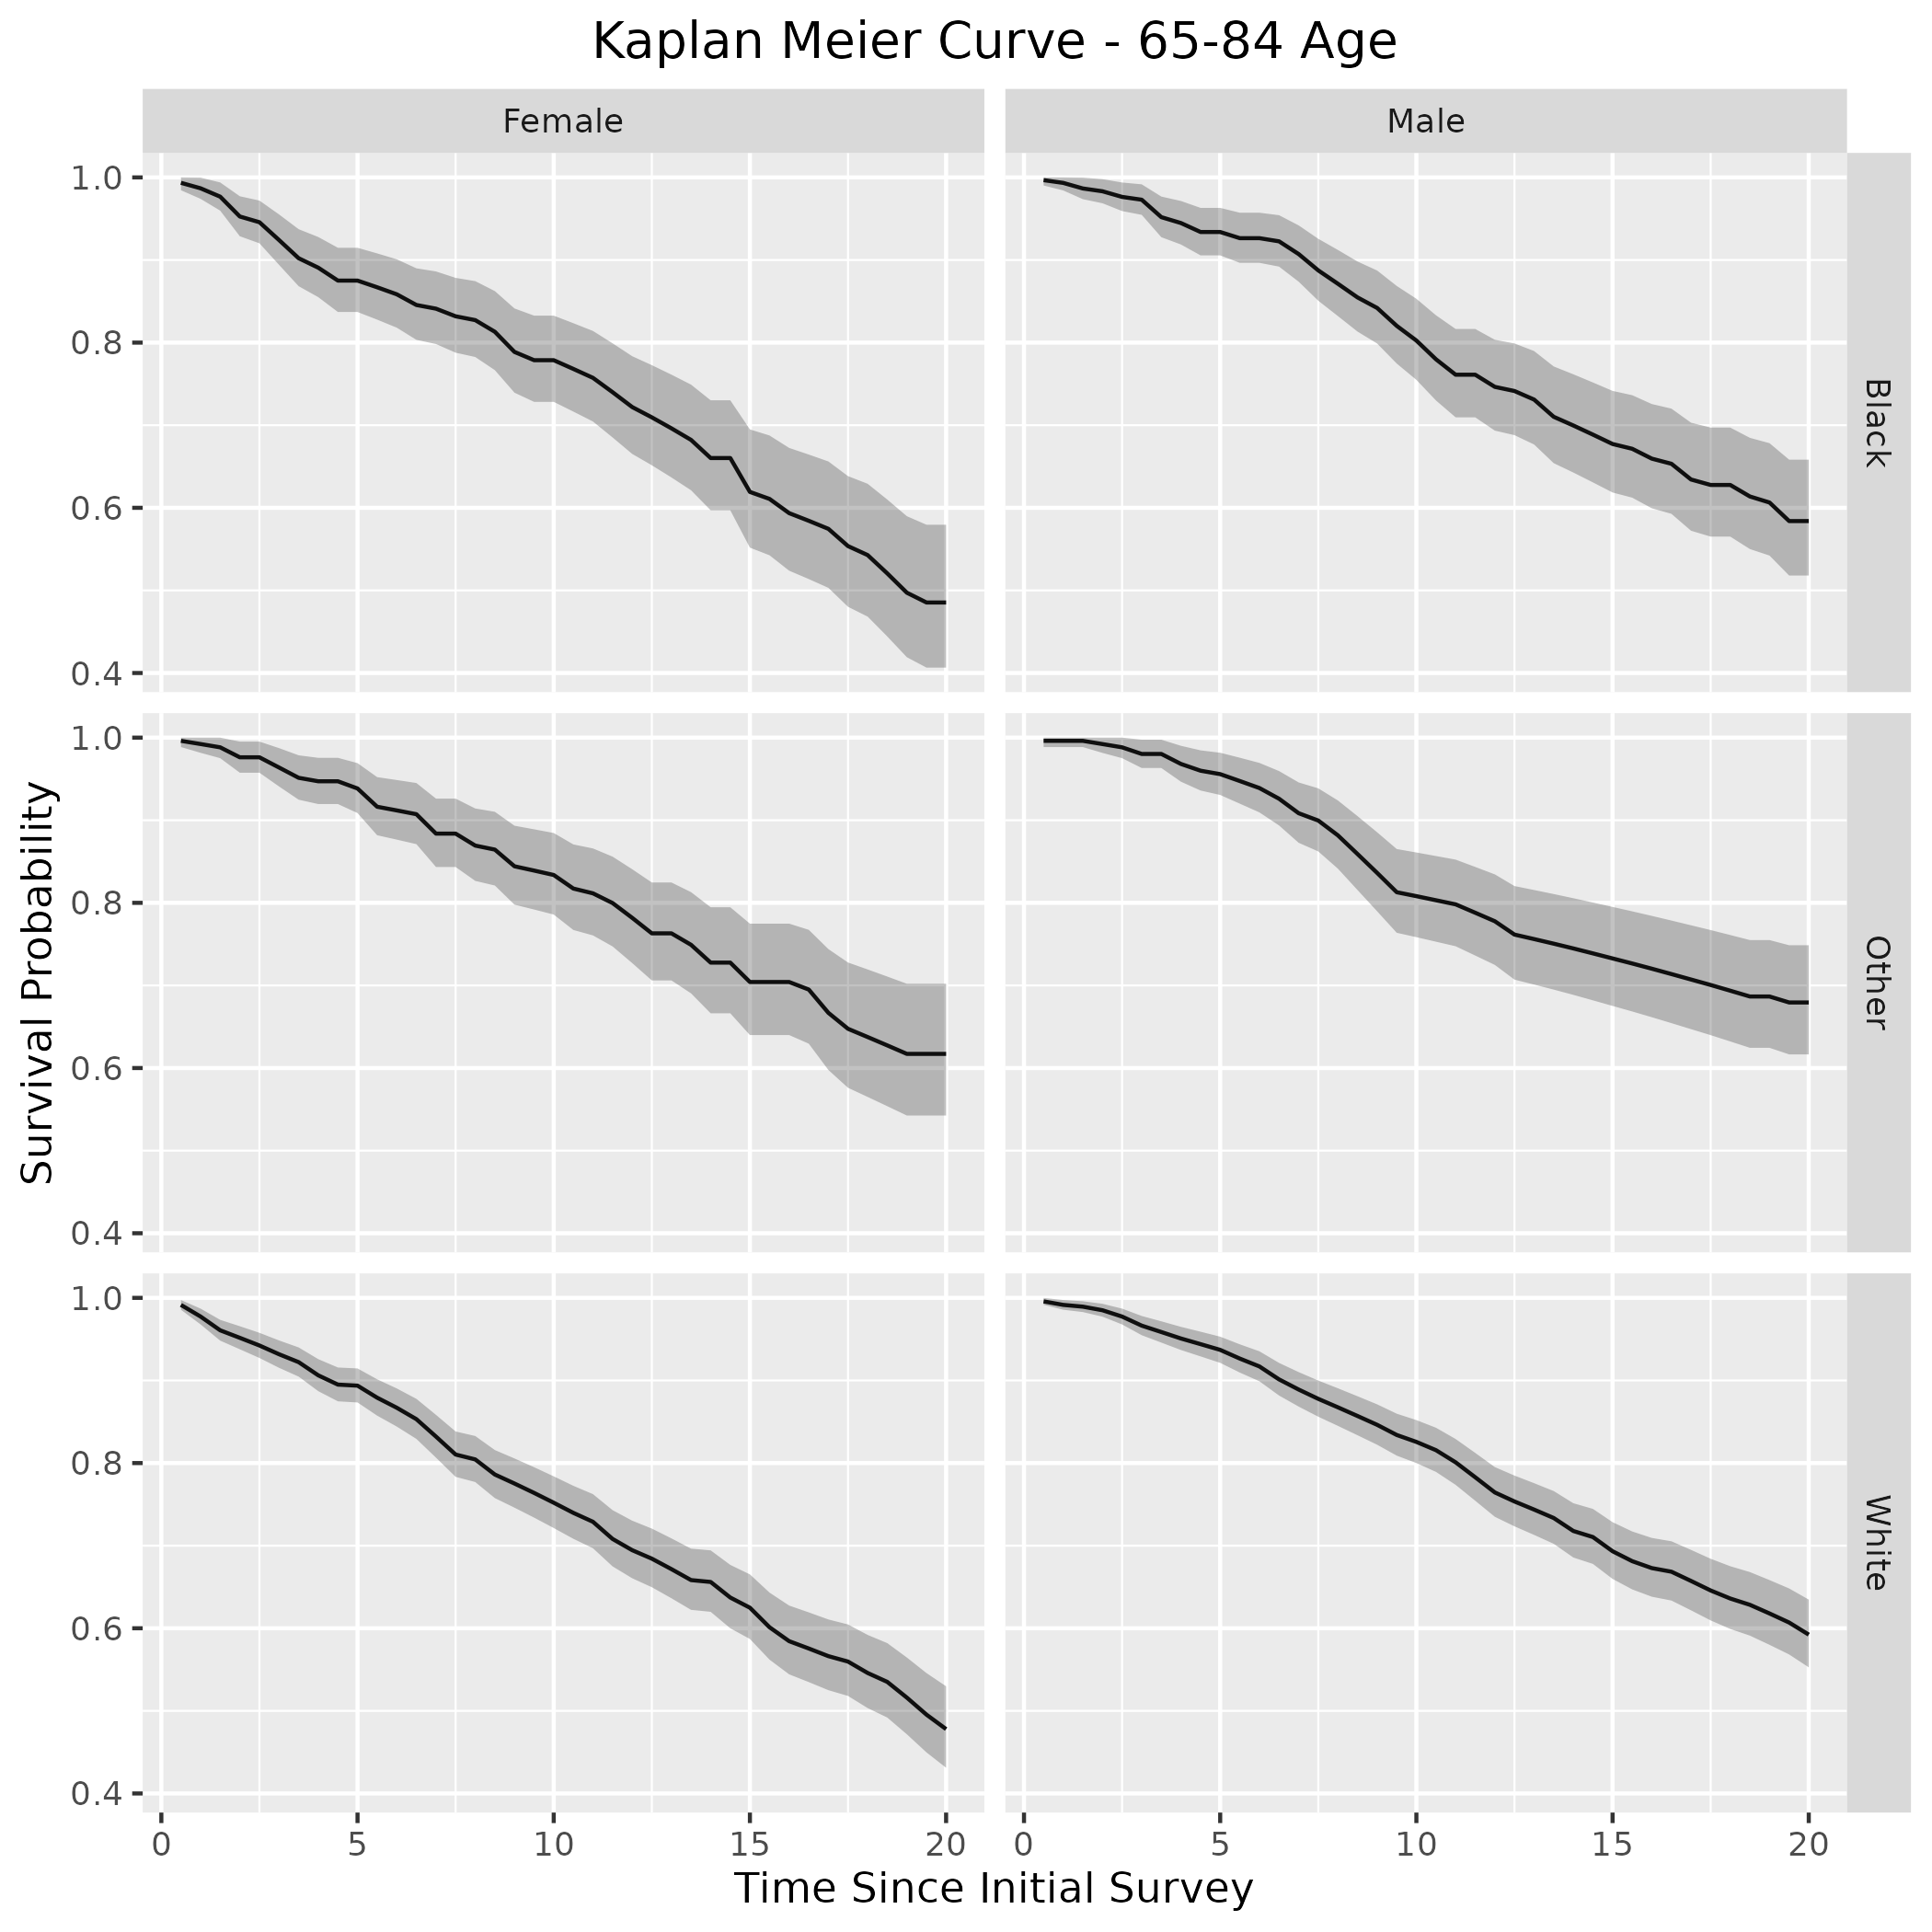
\includegraphics{./Rmarkdown_Plots/SurvProbKM_65-84.png}
\caption{Kaplan-Meier plots of the full-population for HA-CVD-CeVD mortality, for ages between 65-84, split by demographic group.}\label{fig:KM65tot}
}
\end{figure}

By splitting the populations into the respective regions of the \(\Delta\) directionality, we can use the different Kaplan-Meier plots to try to identify differences in the survival outcomes. Figures \ref{fig:KM45_deltaregion} and \ref{fig:KM65_deltaregion} show the Kaplan-Meier estimates for the full NHANES population for HA-CVD-CeVD mortality, split by \(\Delta\) directionality and demographic group, for the age range 45-64 and 65-84, respectively. With the broad confidence intervals, all of the different \(\Delta\) directionality regions overlap, for all demographic groups and both age range groups (where \(\hat{S}(t)\neq 1\)).

\begin{figure}
\hypertarget{fig:KM45_deltaregion}{%
\centering
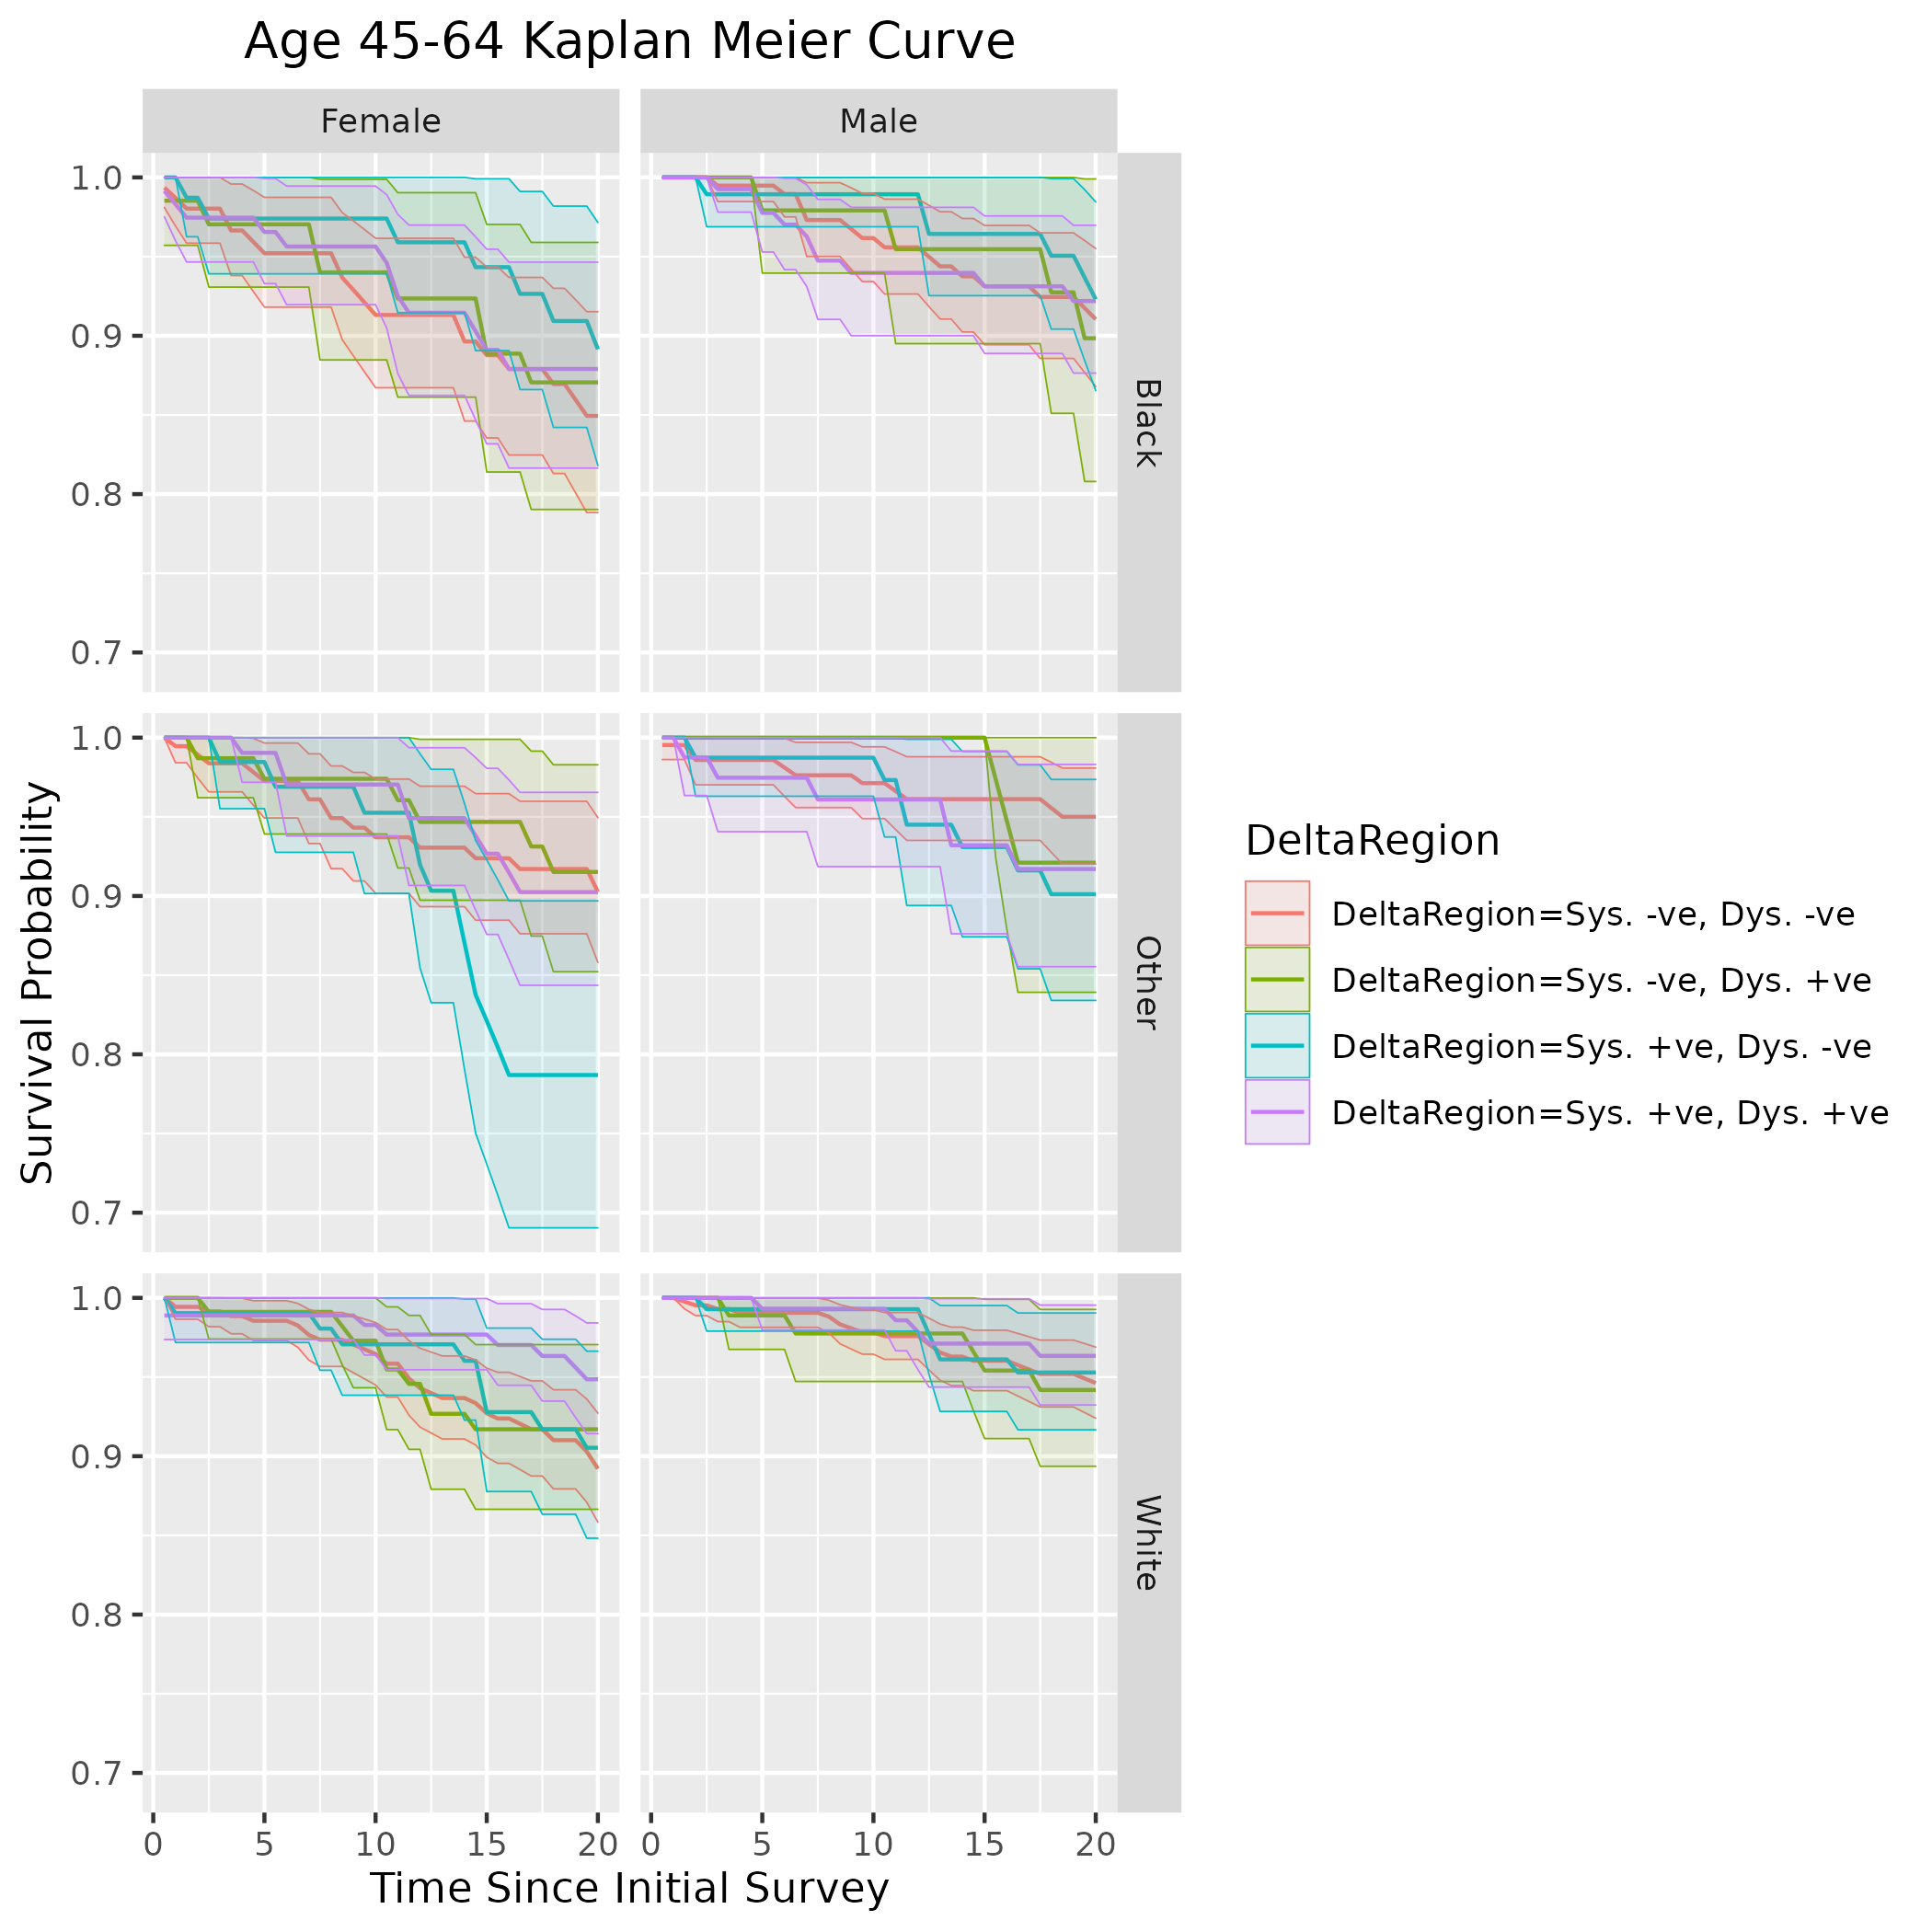
\includegraphics{./Rmarkdown_Plots/SurvProbKM_Delta_45-65.png}
\caption{Kaplan-Meier plots of the full-population for HA-CVD-CeVD mortality, for ages between 45-64, split by demographic group and region in systolic-diastolic \(\Delta\) space.}\label{fig:KM45_deltaregion}
}
\end{figure}

\begin{figure}
\hypertarget{fig:KM65_deltaregion}{%
\centering
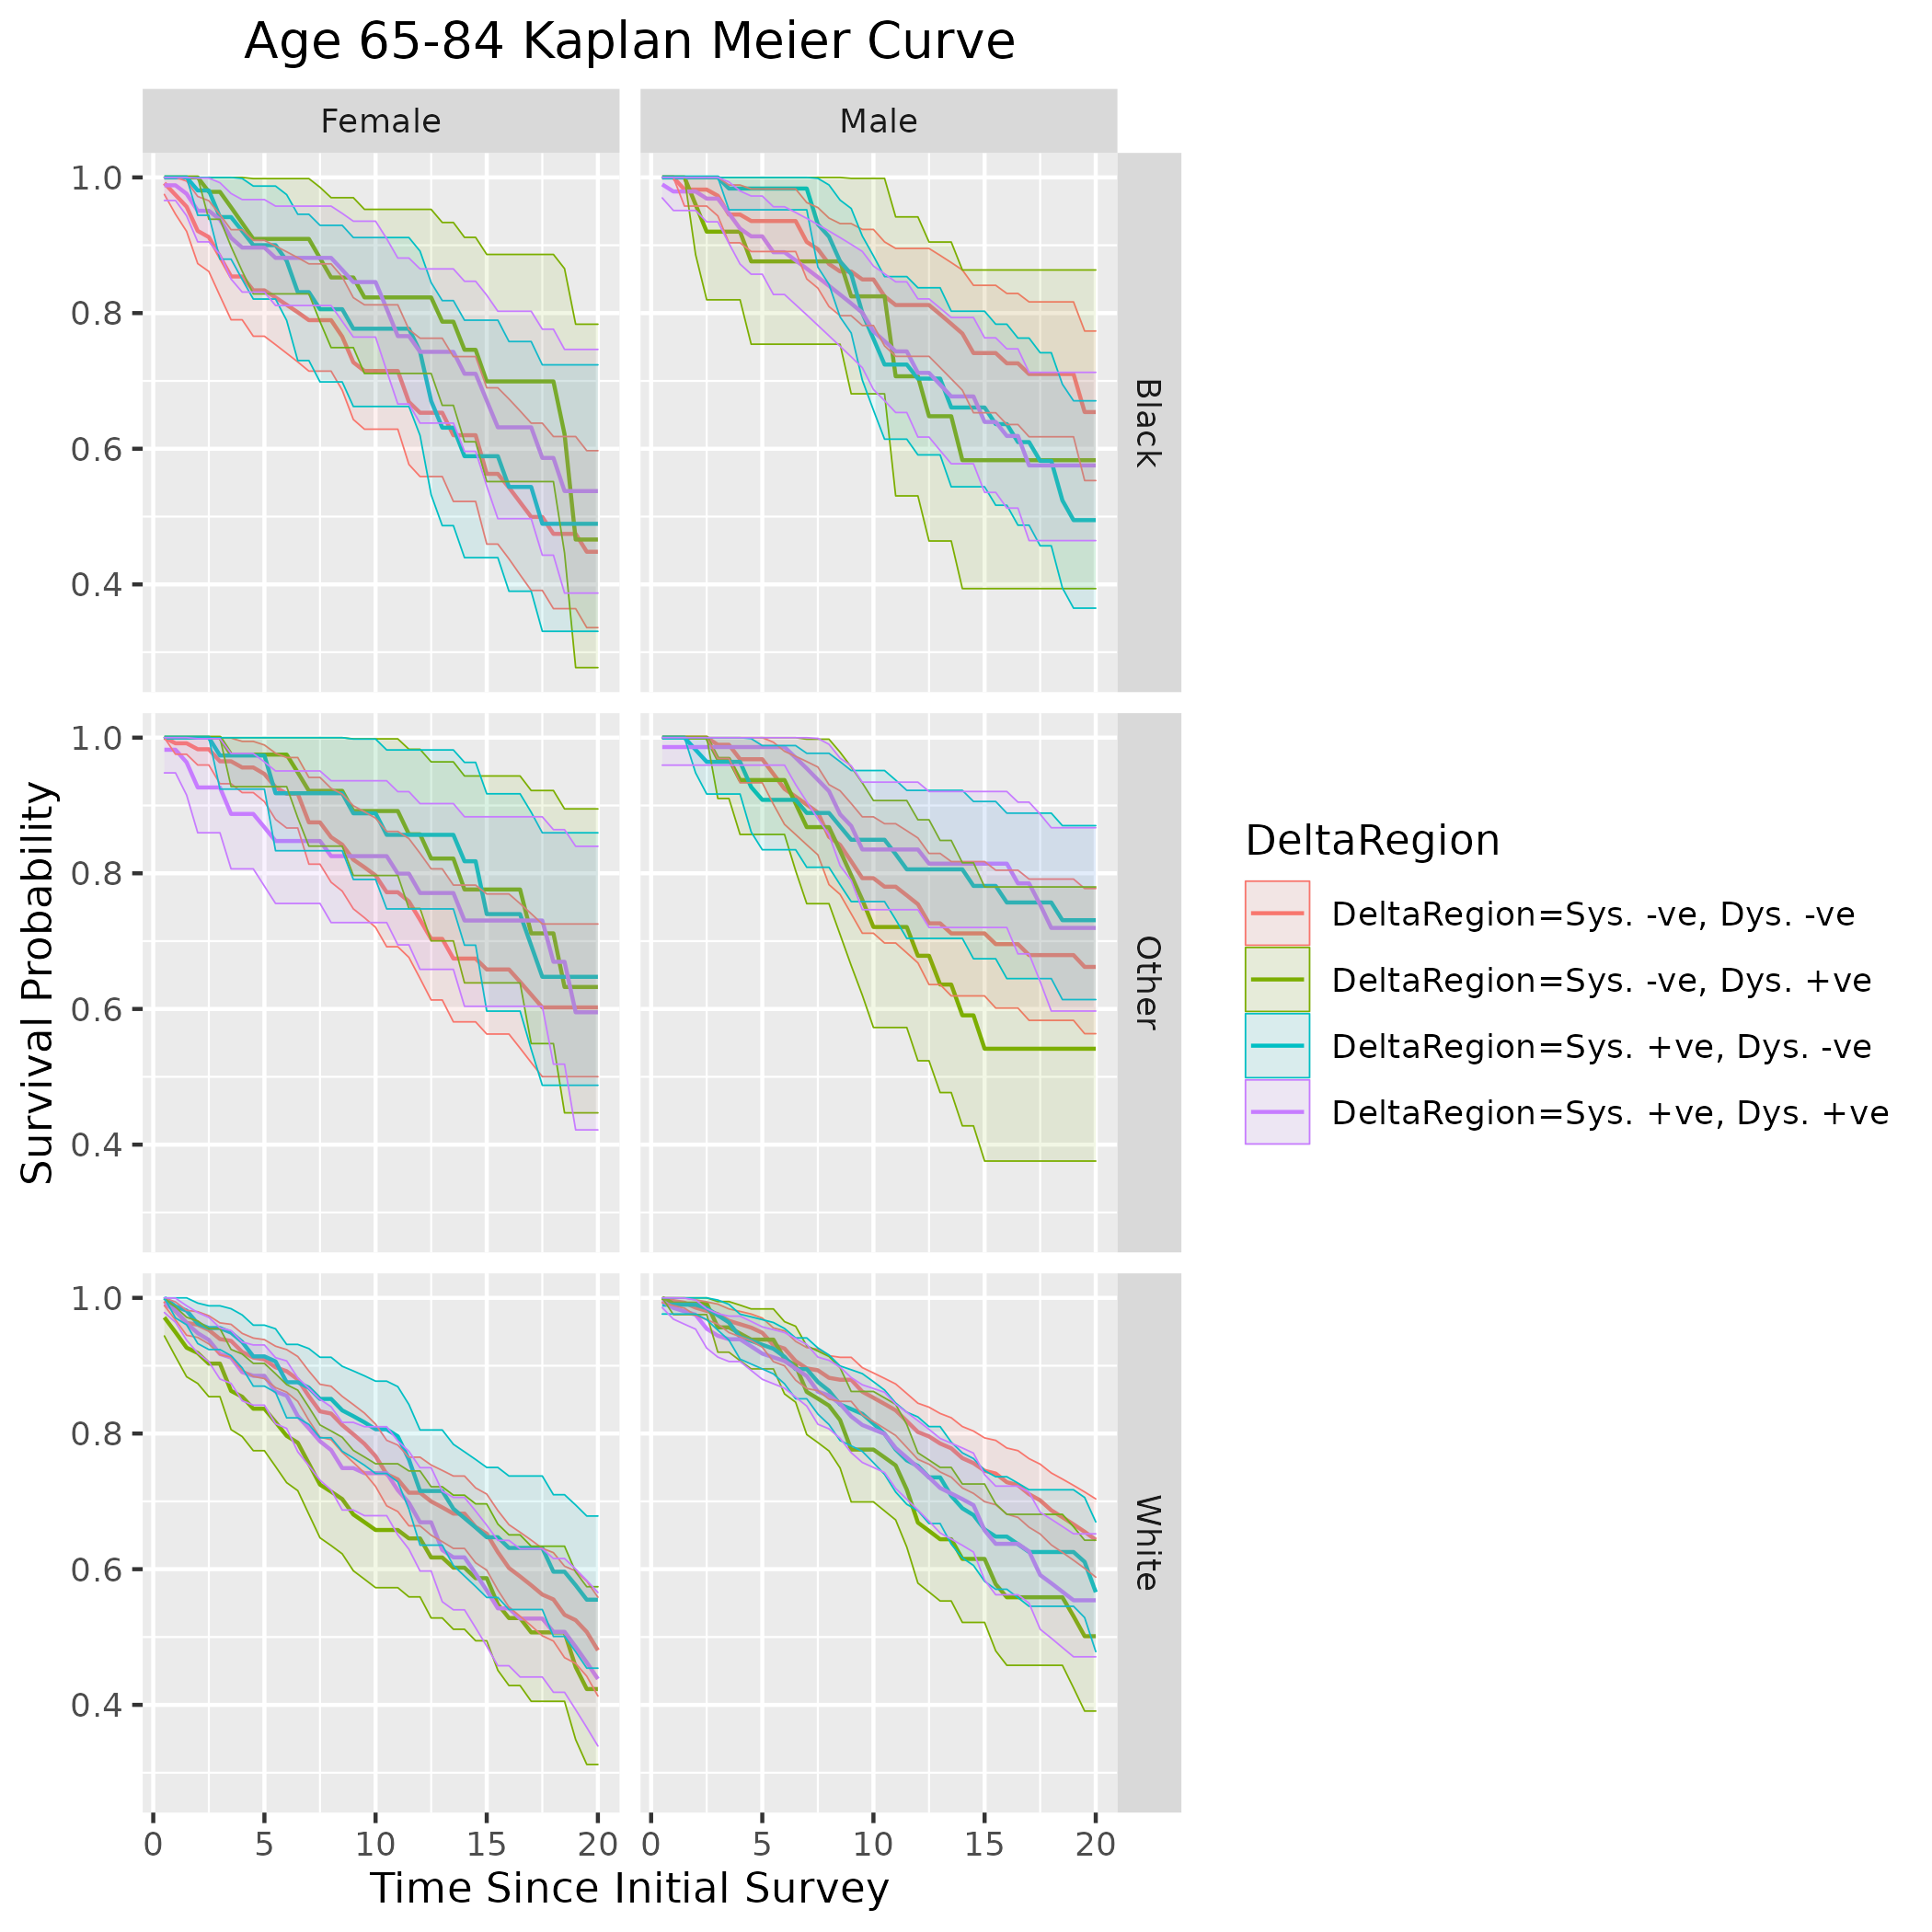
\includegraphics{./Rmarkdown_Plots/SurvProbKM_Delta_65-85.png}
\caption{Kaplan-Meier plots of the full-population for HA-CVD-CeVD mortality, for ages between 65-84, split by demographic group and region in systolic-diastolic \(\Delta\) space.}\label{fig:KM65_deltaregion}
}
\end{figure}

We further quantify this insignificant relationship between \(\Delta\) directionality and survival outcome via the use of a Cox's Proportional Hazards (CPH) model. Via the use of the `coxph' function in the `survival' R package, we fit (using MLE) a CPH model. The covariates used in the model are \(\Delta\) directionality region, gender, ethnicity and age. Table \ref{tab:DeltaDir} shows the summary of the model fit, which reflects that being in different \(\Delta\) directionality regions has a non-statistically significant influence on survival outcomes. As shown in the remainder of this article, ethnicity, gender and age are shown to have statistically significant effects on survival outcome.

\begin{table}

\caption{\label{tab:DeltaDir}Parameters for distribution of blood pressure, for the full population}
\centering
\begin{tabular}[t]{lrrrrr}
\toprule
covariate & coef & exp(coef) & se(coef) & z & Pr(>|z|)\\
\midrule
DeltaRegionSys. -ve, Dys. +ve & 0.0468181 & 1.0479314 & 0.0738547 & 0.6339213 & 0.5261322\\
DeltaRegionSys. +ve, Dys. -ve & -0.0021526 & 0.9978497 & 0.0688467 & -0.0312669 & 0.9750567\\
DeltaRegionSys. +ve, Dys. +ve & -0.0558931 & 0.9456403 & 0.0634611 & -0.8807454 & 0.3784556\\
GenderMale & -0.4125926 & 0.6619319 & 0.0498157 & -8.2823782 & 0.0000000\\
EthnicityWhite & -0.2478299 & 0.7804927 & 0.0613030 & -4.0427047 & 0.0000528\\
\addlinespace
EthnicityOther & -0.1695250 & 0.8440656 & 0.0745991 & -2.2724800 & 0.0230575\\
age & 0.0995937 & 1.1047220 & 0.0019693 & 50.5727891 & 0.0000000\\
\bottomrule
\end{tabular}
\end{table}

Finally, we wish to confirm that the perfomance of the model does not depend on the directionality of \(\Delta\). Figure \ref{fig:DeltaAUCs} plots the AUC values of 10-year HA-CVD-CeVD mortality for the all-covariate mean blood pressure-based model trained on the full NHANES population, split by the two age-ranges (45-64 and 65-84) and demographic groups. There is no clear trend between mode performance for the different regions of \(\Delta\) directionality.

\begin{figure}
\hypertarget{fig:DeltaAUCs}{%
\centering
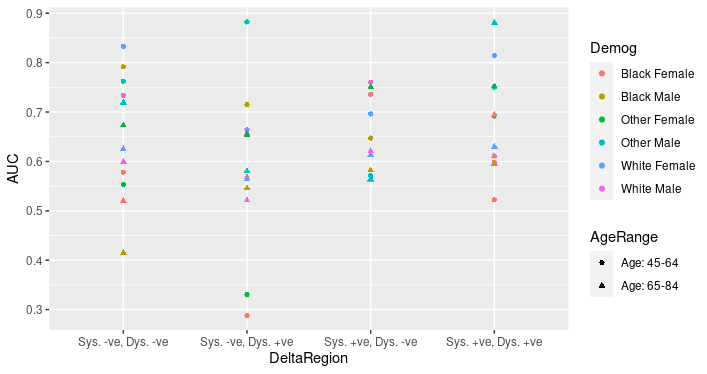
\includegraphics{./Rmarkdown_Plots/DeltaDirection_AUCs.png}
\caption{AUC values of the full-population, all covariate model with the mean blood pressure model, based on HA-CVD-CeVD 10-year mortality.}\label{fig:DeltaAUCs}
}
\end{figure}

\hypertarget{references}{%
\section*{References}\label{references}}
\addcontentsline{toc}{section}{References}

\hypertarget{refs}{}
\begin{CSLReferences}{1}{0}
\leavevmode\vadjust pre{\hypertarget{ref-ostchega2003national}{}}%
Ostchega, Yechiam, Ronald J Prineas, Ryne Paulose-Ram, Carlene M Grim, Grace Willard, and Doreen Collins. 2003. {``National Health and Nutrition Examination Survey 1999-2000: Effect of Observer Training and Protocol Standardization on Reducing Blood Pressure Measurement Error.''} \emph{Journal of Clinical Epidemiology} 56 (8): 768--74.

\end{CSLReferences}

\end{document}
